
\documentclass[a4paper,12pt,twoside]{report}

\usepackage[left=40mm,right=20mm,top=2cm,bottom=3cm]{geometry}
\usepackage{amssymb}
\usepackage{amsmath}
\usepackage{float} 
\usepackage[font=footnotesize]{subcaption}
\usepackage[font=footnotesize]{caption}
\usepackage[table]{xcolor}
\usepackage{tabularx}
\usepackage{longtable}
\usepackage{ltxtable}
\usepackage{booktabs}
\usepackage{comment}
\PassOptionsToPackage{obeyspaces}{url}
\usepackage{url}
\usepackage{calc}
\usepackage{appendix}
\usepackage[noadjust]{cite}
\usepackage[figuresright]{rotating}
\usepackage{IEEEtrantools}



\def\tablename{Table}


\newcolumntype{M}[1]{@{}>{\centering\arraybackslash}m{#1}@{}}
\newcolumntype{C}{>{\centering\arraybackslash}X}

 
\usepackage{algorithmicx}
\usepackage{algorithm,algpseudocode}
\usepackage{eurosym}

\renewcommand{\algorithmicrequire}{\textbf{Input:}}
\renewcommand{\algorithmicensure}{\textbf{Output:}}
\let\oldReturn\Return
\renewcommand{\Return}{\State\oldReturn}

\setcounter{secnumdepth}{5}

\definecolor{Orange8}{RGB}{153,102,51}
\definecolor{SeaBlue}{RGB}{0,102,204}
\definecolor{Gray7}{RGB}{102,102,102}



\usepackage{graphicx}
\usepackage{verbatim}
\usepackage{latexsym}
%\usepackage{mathchars}


\newcommand{\normallinespacing}{\renewcommand{\baselinestretch}{1.5} \normalsize}

%\input{blocked.sty}


\makeatletter
\def\chapapp2{Chapter}

\def\appendix{\par
 \setcounter{chapter}{0}
 \setcounter{section}{0}
 \def\chapapp2{Appendix}
 \def\@chapapp{Appendix}
 \def\thechapter{\Alph{chapter}}}

\def\ps@uheadings{\let\@mkboth\markboth
\def\@evenhead{\protect\underline{\protect\makebox[\textwidth][l]
		{\sl\rightmark\hfill\rm\thepage}}}
\def\@oddfoot{}
\def\@evenfoot{}
\def\@oddhead{\protect\underline{\protect\makebox[\textwidth][l]
		{\rm\thepage\hfill\sl\rightmark}}}
\def\chaptermark##1{\markboth {\ifnum \c@secnumdepth >\m@ne \chapapp2\ \thechapter. \ \fi ##1}{}}%

\def\sectionmark##1{\markright {\ifnum \c@secnumdepth >\z@
   \thesection. \ \fi ##1}}}
\makeatother




%\input{boxit.sty}
\pagestyle{empty}

\setlength{\parskip}{2ex plus 0.5ex minus 0.2ex}
\setlength{\parindent}{0pt}

\makeatletter  

\linespread{1.5}
\def\submitdate#1{\gdef\@submitdate{#1}}

\def\maketitle{
  \begin{titlepage}{
    \Large \bf \@title \par
  }
  \par
  {\Large \@author}
  \par

A thesis submitted in partial fulfillment of the requirements 
 \linebreak
for the degree of Doctor of Philosophy
  \vfil


    \Large The University of Sheffield \\

   Faculty of Engineering  \\
 
    Department of Electronic \& Electrical Engineering\\
\vskip 2 cm
   Submission Date: \@submitdate
\vskip 2 cm
    \rm
  \end{titlepage}
}

\def\titlepage{
  \newpage
  \centering
  \linespread{1}
  \normalsize
  \vbox to \vsize\bgroup\vbox to 9in\bgroup
}
\def\endtitlepage{
  \par
  \kern 0pt
  \egroup
  \vss
  \egroup
  \clearpage
}

\def\abstract{
  \begin{center}{
   \Huge \bf Abstract}
  \end{center}
  \small

  \linespread{1.5}
  \normalsize
}
\def\endabstract{
  \par
}

\newenvironment{acknowledgements}{
  \clearpage
  \begin{center}{
    \Huge  \bf Acknowledgements}
  \end{center}
  \small
  \linespread{1.5}
  \normalsize
}{\cleardoublepage}
\def\endacknowledgements{
  \par
}

\newenvironment{dedication}{
  \clearpage
  \begin{center}{
    \Huge  \bf Dedication}
  \end{center}
  \small
  \linespread{1.5}
  \normalsize
}

\newenvironment{appendix1}{
  \clearpage
  \begin{center}{
    \Huge \bf Appendix}
  \end{center}
  \small
  \linespread{1.5}
  \normalsize
}

\newenvironment{Statement_of_Originality}{
  \clearpage
  \begin{center}{
    \Huge  \bf Statement of Originality}
  \end{center}
  \small
  \linespread{1.5}
  \normalsize
}


\newenvironment{List_of_Publications}{
  \clearpage
    \pagestyle{uheadings}
  \begin{center}{
    \Huge  \bf List of Publications}
  \end{center}
  \small
  \linespread{1.5}
  \normalsize
}

\def\preface{
    \pagenumbering{roman}
    \pagestyle{plain}
    \doublespacing
}

\def\body{
    \clearpage    
    \pagestyle{uheadings}
\addcontentsline{toc}{chapter}{Table of Contents}
    \tableofcontents
    \clearpage
    \pagestyle{uheadings}
\addcontentsline{toc}{chapter}{List of Tables}
    \listoftables
    \clearpage
    \pagestyle{uheadings}
\addcontentsline{toc}{chapter}{List of Figures}
    \listoffigures
\clearpage
    \pagestyle{uheadings}
    \setlength{\nomlabelwidth}{3cm}                                                   


\newcommand{\nomunit}[1]{%
\renewcommand{\nomentryend}{\hspace*{\fill}#1}}


% first letter a is for Greek Symbols

\nomenclature[a,01]{$\alpha$}{Albedo of ground}  
\nomenclature[a,02]{$\gamma$}{Inclination angle of PV cell, $\gamma \in[0^{\mathrm{o}},90^{\mathrm{o}}]$}  
\nomenclature[a,03]{$\Delta_1$}{Gain of adding the $1^{\mathrm{st}}$ PV cell, cf. (\ref{Delta_1})}
\nomenclature[a,04]{$\Delta_n$}{Gain of adding the $n^{\mathrm{th}}$ PV cell, $n\in\{2, ..., N\}$, cf. (\ref{Delta_n})}
\nomenclature[a,05]{$\delta_d$}{Declination angle, cf. (\ref{delta})}
\nomenclature[a,06]{$\zeta_t$}{Zenith angle, cf. (\ref{zenith})}
\nomenclature[a,07]{$\eta$}{Energy conversion efficiency of PV cell}
\nomenclature[a,08]{$\theta$}{Orientation angle of PV cell, $\theta\in[-90^{\mathrm{o}},90^{\mathrm{o}}]$}
\nomenclature[a,09]{$\theta^*$}{Optimal orientation angle of PV cell, $\theta^*\in[-90^{\mathrm{o}},90^{\mathrm{o}}]$}
\nomenclature[a,10]{$\theta_n$}{Orientation angle of PV cell $n$, $\theta_n\in[-90^{\mathrm{o}},90^{\mathrm{o}}]$} 
\nomenclature[a,11]{$\theta_n^*$}{Optimal orientation angle of PV cell $n$, $\theta_n^*\in[-90^{\mathrm{o}},90^{\mathrm{o}}]$} 
\nomenclature[a,12]{$\lambda(t)$}{Density parameter of Poisson distributed random variable at time step $t$, cf. (\ref{P})}
\nomenclature[a,13]{$\mu$}{Precision of the discretization of the energy values/ battery states}
\nomenclature[a,14]{$\rho$}{Resistivity of the distribution line } %\nomunit{[$\mathrm{\Omega}$ m]}
\nomenclature[a,15]{$\tau$}{Duration of one time step } %  \nomunit{[s]}
\nomenclature[a,16]{$\omega_t$}{Hour angle, cf. Figure \ref{hour_angle_graph}}



% first letter b is for Roman symbols capital letter


\nomenclature[b,01]{$A$}{Total surface area of $N$ PV cells}% \nomunit{[$\mathrm{m}^2$]} 
\nomenclature[b,02]{$A_c$}{Cross-sectional area of the distribution line}% \nomunit{[$\mathrm{m}^2$]}
\nomenclature[b,03]{$A_t$}{Anisotropy index at time step $t$, cf. (\ref{At})}  
\nomenclature[b,04]{$AOI_{\theta}(t)$}{Angle of incidence of a PV cell deployed with orientation angle $\theta$ at time step $t$, cf. (\ref{allgemein_AOI})}  
\nomenclature[b,05]{$B$}{Number of BSs in the square area of $l^2$ square meters, cf. Figure \ref{fig:1}}  
\nomenclature[b,11]{$BS_i$}{BS with index $i$}  
\nomenclature[b,12]{$C$}{Power loss coefficient per $l$ meters of distribution line}% \nomunit{[$\mathrm{\Omega}$]}  
\nomenclature[b,13]{$C(t)$}{Energy consumption of the BS at time step $t$, cf. Figures \ref{constant_allgemein} - \ref{residential_allgemein}}% \nomunit{[J]} 
\nomenclature[b,14]{$C_{\mathrm{bus}}(t)$}{Business-area traffic load profile at time step $t$, cf. Figure \ref{all_consumption_profiles}}  
\nomenclature[b,15]{$C_{\mathrm{con}}(t)$}{Constant traffic load profile at time step $t$, cf. Figure \ref{all_consumption_profiles}}  
\nomenclature[b,21]{$C_{\mathrm{res}}(t)$}{Residential-area traffic load profile at time step $t$, cf. Figure \ref{all_consumption_profiles}} 
\nomenclature[b,22]{$DHI_t$}{Diffuse horizontal irradiance at time step $t$, obtained from PVGIS \cite{PVGIS}}  
\nomenclature[b,23]{$DNI_t$}{Direct normal irradiance at time step $t$, obtained from PVGIS \cite{PVGIS}}  
\nomenclature[b,24]{$E$}{Set of edges in the graph/cellular network, cf. (\ref{V_and_E})} 
\nomenclature[b,25]{$E_{\mathrm{con}}$}{Solar constant set at $1367\frac{\mathrm{W}}{\mathrm{m}^2}$ \cite{Solar_Cell_declination_inclination_angle}} 
\nomenclature[b,26]{$E_d$}{Extraterrestrial radiation on day $d$, cf. (\ref{extra})} 
\nomenclature[b,31]{$G(t)$}{Energy generation of the PV cell/cells at time step $t$}  
\nomenclature[b,32]{$G^{\text{original}}_{\theta,N}(t)$}{Energy generated by one PV cell installed with $\theta$ ($N$ is the total number of PV cells) at time step $t$, cf. (\ref{normalization})}  
\nomenclature[b,330]{$G_{\theta,N}(t)$}{Normalized energy generated by one PV cell installed with $\theta$ ($N$ is the total number of PV cells) at time step $t$, cf. (\ref{norma})} 
\nomenclature[b,335]{$\tilde{G}_{\theta,1}(t)$}{Closest multiple of $\mu$ from $G_{\theta,1}(t)$} 
\nomenclature[b,34]{$G_{(\theta_1, ..., \theta_N)}(t)$}{Normalized total energy generated by $N$ PV cells installed with $\theta_1, ....,\theta_N$ at time step $t$, cf. (\ref{nor})}   
\nomenclature[b,35]{$GHI_t$}{Global horizontal irradiance at time step $t$, obtained from PVGIS \cite{PVGIS}}   
\nomenclature[b,41]{$I_{\theta}(t)$}{Irradiance on PV cell installed with orientation angle $\theta$ at time step $t$, cf. (\ref{I1})} 
\nomenclature[b,42]{$I_{b_\theta}(t)$}{Direct-beam irradiance at time step $t$, cf. (\ref{I4})} 
\nomenclature[b,43]{$I_{d_\theta}(t)$}{Sky-diffuse irradiance at time step $t$, cf. (\ref{reindl})} 
\nomenclature[b,44]{$I_{g}(t)$}{Ground-reflected irradiance at time step $t$, cf. (\ref{I3})} 
\nomenclature[b,45]{$I_{\mathrm{ele}}$}{Electric current traveling through the distribution line}% \nomunit{[A]}
\nomenclature[b,51]{$L$}{Number of loops in simulation algorithm}
\nomenclature[b,52]{$M$}{Total normalized renewable power received at the deficit BSs during the two time steps}% \nomunit{[W]}
\nomenclature[b,53]{$N$}{Number of PV cells at the BS}  
\nomenclature[b,54]{$P_{\mathrm{loss}}$}{Power loss in the transmission due to resistive heating, cf. (\ref{loss})}% \nomunit{[W]}
\nomenclature[b,55]{$S_{\max}$}{Number of battery energy states, cf. (Algorithm \ref{mar} line: \ref{battery_stages})} 
\nomenclature[b,61]{$S_{\mathrm{Shift}}$}{New battery state after $\tilde{G}_{\theta,1}(t)$ is added and $c_{\mathrm{con}}$ is subtracted, cf. (Algorithm \ref{mar} line: \ref{she})} 
\nomenclature[b,62]{$S_{\mathrm{UE}}(\theta)$}{Number of UEs served per day by the BS, cf. (\ref{PPP})}  
\nomenclature[b,63]{$\overline{S_{\mathrm{UE}}}(\theta)$}{Average number of UEs served per day by the BS, cf. (\ref{PPP})}  
\nomenclature[b,64]{$T$}{Number of time steps per day}    
\nomenclature[b,65]{$V$}{Set of vertices in the graph/ cellular network, cf. (\ref{V_and_E})}  
\nomenclature[b,66]{$V_{\mathrm{ele}}$}{Electric potential in the distribution line}% \nomunit{[V]}


			

% first letter c is for Roman symbols small letter 
\nomenclature[c,001]{$a_\theta(t)$}{Available energy in the battery at the beginning of time step $t$, cf. (\ref{available})} %\nomunit{[J]}
\nomenclature[c,001]{$a_t$}{Part of $\cos(AOI_{\theta}(t))$ that is independent of $\theta$, cf. (\ref{a_t})} 
\nomenclature[c,001]{$b_t$}{Part of $\cos(AOI_{\theta}(t))$ that is multiplied by  $\sin(\theta)$, cf.  (\ref{b_t})} 
\nomenclature[c,011]{$b_\theta(t)$}{Stored energy in the battery at the end of time step $t$, cf. (\ref{bat})} %\nomunit{[J]}
\nomenclature[c,012]{$b_{\mathrm{begin}}$}{Amount of energy stored in the battery at time step $0$}  %\nomunit{[J]}
\nomenclature[c,013]{$b_{\mathrm{max}}$}{Battery capacity}  	%\nomunit{[J]}
\nomenclature[c,014]{$b_0$}{Power surplus value, $b_0\in \mathbb{R}^+$} %\nomunit{[W]}}
\nomenclature[c,015]{$b_1$}{Power deficit value, $b_1\in \mathbb{R}^-$} %\nomunit{[W]}}
\nomenclature[c,016]{$\hat{b}_0$}{Normalize power surplus value with respect to $\mathrm{max}\{b_0,\lvert b_1 \rvert\}$, cf. (\ref{normal})} %\nomunit{[W]}} %
\nomenclature[c,017]{$\hat{b}_1$}{Normalize power deficit value with respect to $\mathrm{max}\{b_0,\lvert b_1 \rvert\}$, cf. (\ref{normal})}  %\nomunit{[W]}
\nomenclature[c,021]{$c_\theta(t)$}{Load-dependent energy consumption of the BS at time step t, cf. (\ref{PPP3})} 		%\nomunit{[J]}									
\nomenclature[c,022]{$c_{\mathrm{con}}$}{Load-independent part of the energy consumption at the BS in one time step}%\nomunit{[J]}
\nomenclature[c,023]{$c_i$}{Cluster allocation value of $BS_i$, $c_i\in\{0,1\}$}  
\nomenclature[c,024]{$c_t$}{Part of $\cos(AOI_{\theta}(t))$ that is multiplied by  $\cos(\theta)$, cf.  (\ref{c_t})}
\nomenclature[c,025]{$c_{\mathrm{UE}}$}{Average energy consumption of the BS to serve one UE during a time step}%	\nomunit{[J]}	 
\nomenclature[c,026]{$d$}{Day of the year with $1^{\mathrm{st}}$ of January is $d=1$} 
\nomenclature[c,031]{$d\big((i,j)\big)$}{Normalize Euclidean distance between $BS_i$ and $BS_j$ with respect to $l$ meters, cf. (\ref{equ_y})} 
\nomenclature[c,041]{$e$}{Edge $e$ in a graph}
\nomenclature[c,043]{$f^t\big((i,j)\big)$}{Power flow on the directed edge from $BS_i$ to $BS_j$ at time step $t$ or second power of the current flow on the directed edge from $BS_i$ to $BS_j$ at time step $t$}% \nomunit{[W]}
\nomenclature[c,044]{$\hat{f}^t\big((i,j)\big)$}{Normalize power flow value with respect to $\mathrm{max}\{b_0,\lvert b_1 \rvert\}$ on the directed edge from $BS_i$ to $BS_j$ at time step $t$, cf. (\ref{normal})}%\nomunit{[W/$\mathrm{A}^2$]}
\nomenclature[c,045]{$f(\theta_1, ..., \theta_N)$}{Normalized energy drawn from the grid, Optimization objective, cf. (\ref{optimization_objective})}
\nomenclature[c,046]{$l$}{Side length of the square in Fig \ref{fig:1}}% \nomunit{[m]} 
\nomenclature[c,047]{$lat$}{Latitude of location}  
\nomenclature[c,048]{$lon$}{Longitude of location}  
\nomenclature[c,049]{$l(t)$}{Number of UEs connected to the BS at time step $t$, cf.  (\ref{PPP1})} 
\nomenclature[c,060]{$n$}{Index of BS, $n\in\{1, ..., N\}$}      
\nomenclature[c,061]{$p_i^t$}{Surplus/Deficit power of $BS_i$ at time step $t$, cf. (\ref{p_values})}% \nomunit{[W]}
\nomenclature[c,062]{$q$}{Probability that two BSs are connected by a distribution line, $q \in [0,1]$} 
\nomenclature[c,063]{$s_\theta(t)$}{Number of served UEs by the BS at time step $t$, cf. (\ref{PPP2})} 
\nomenclature[c,064]{$t$}{Index of time step, $t\in\{1, ..., T\}$}   
\nomenclature[c,065]{$v$}{Vertex $v$ in a graph}


% first letter R is for superscript
\nomenclature[r,02]{$^*$}{Optimal value}  

% first letter S is for subscripts  
\nomenclature[s,01]{$_{\theta}$}{Parameter depends on the PV cell orientation angle $\theta$}
\nomenclature[s,02]{$_{d}$}{Parameter depends on the day of the year with $1^{\mathrm{st}}$ of January is $d=1$}  
\nomenclature[s,03]{$_{i}$}{Index of BS, $i\in\{1, ..., B\}$}
\nomenclature[s,04]{$_{j}$}{Index of BS, $j\in\{1, ..., B\}$}
\nomenclature[s,05]{$_n$}{Index of PV cell, $n\in\{1, ..., N\}$} 
\nomenclature[s,06]{$_t$}{Index of time step, $t\in\{1, ..., T\}$}  

  
 
                  







 %first letter Z is for Acronyms 

\nomenclature[z,02]{A*STAR}{Agency for Science, Technology and Research in Singapore}
\nomenclature[z,02]{BS}{Base station}
\nomenclature[z,02]{AC}{Alternating current}
\nomenclature[z,02]{DC}{Direct current}
\nomenclature[z,02]{MILPP}{Mixed-integer linear programming problem}
\nomenclature[z,02]{GIS}{Geographic information system}
\nomenclature[z,02]{PV}{Photovoltaic}
\nomenclature[z,02]{PVGIS}{Photovoltaic geographic information system}
\nomenclature[z,02]{SINR}{Signal-to-interference-plus-noise ratio}
\nomenclature[z,02]{UE}{User equipment}

  %first letter X is for Other Symbols

\nomenclature[x,00]{$\forall$}{For all} 
\nomenclature[x,12]{$\lfloor x \rceil$}{$x$ is rounded to the nearest integer value} 
\nomenclature[x,13]{$\lfloor x \rfloor$}{$x$ is rounded down to the nearest integer value} 
\nomenclature[x,20]{$\mathbb{N}$}{Set of natural numbers} 
\nomenclature[x,21]{$\mathbb{R}$}{Set of real numbers}
\nomenclature[x,21]{$\mathbb{Z}$}{Set of integer numbers}
\nomenclature[x,30]{$\mathbb{P}(X=x)$}{Probability that the random variable $X$ is equal to $x$}
\nomenclature[x,31]{$\mathbb{P}(X\geq x)$}{Probability that the random variable $X$ is not less than the value $x$} 
\nomenclature[x,32]{$X:=\mathrm{PD}(\lambda)$}{$X$ is a Poisson distributed random variable with density parameter $\lambda$ }%\nomunit{[$\lambda \in \mathbb{R}^+$]}
\nomenclature[x,40]{$G<<C$}{Energy generation of PV cell/cells is significantly smaller than energy consumption of BS} 
\nomenclature[x,41]{$G<C$}{Energy generation of PV cell/cells is slightly smaller than energy consumption of BS} 
\nomenclature[x,42]{$G>C$}{Energy generation of PV cell/cells is slightly greater than energy consumption of BS} 
\nomenclature[x,43]{$G>>C$}{Energy generation of PV cell/cells is significantly greater than energy consumption of BS} 
\nomenclature[x,70]{$\lvert \lvert BS_i - BS_j \rvert \rvert$}{Euclidean distance between $BS_i$ and $BS_j$}% \nomunit{[m]} 
\nomenclature[x,90]{$(i,j)$}{Directed edge from $BS_i$ to $BS_j$} 
\nomenclature[x,01]{$n%! $}{Factorial of non-negative integer $n$, $n \in \mathbb{N}_0$}
  




 
    \pagestyle{plain}
 \clearpage
    \pagestyle{uheadings}
    \doublespacing
}


\renewenvironment{appendices}{
    \pagestyle{uheadings}


  \@resets@pp
  \if@dotoc@pp
    \if@dopage@pp              
      \if@chapter@pp        
        \clear@ppage
      \fi
      \appendixpage
    \else               
       \if@chapter@pp        
         \clear@ppage
       \fi
      \addappheadtotoc
    \fi
  \else
    \if@dopage@pp              
      \appendixpage
    \fi
  \fi
  \if@chapter@pp
    \if@dotitletoc@pp \@redotocentry@pp{chapter} \fi
  \else
    \if@dotitletoc@pp \@redotocentry@pp{section} \fi
    \if@dohead@pp
      \def\sectionmark##1{%
        \if@twoside
        \markright{\@formatsecmark@pp{##1}}
        \else
        \markright{\@formatsecmark@pp{##1}}{}
        \fi}
    \fi
    \if@dotitle@pp
      \def\sectionname{\appendixname}
      \def\@seccntformat##1{\@ifundefined{##1name}{}{\csname ##1name\endcsname\ }%
        \csname the##1\endcsname\ifnum0=\pdfstrcmp{##1}{section}:\fi\quad}
    \fi
  \fi}{
  \@ppsaveapp\@pprestoresec}
\makeatother



\renewcommand{\contentsname}{T\MakeLowercase{able of }C\MakeLowercase{ontents}}

\renewcommand{\listfigurename}{L\MakeLowercase{ist of }F\MakeLowercase{igures}}
\renewcommand{\listtablename}{L\MakeLowercase{ist of }T\MakeLowercase{ables}}
\renewcommand{\appendixname}{List of appendices}
\renewcommand{\appendixpagename}{List of appendices}


\renewcommand\bibname{R\MakeLowercase{eferences}}






% ******************************* Nomenclature *********************************
\RequirePackage[intoc]{nomencl}
\makenomenclature
\renewcommand{\nomgroup}[1]{%
\ifthenelse{\equal{#1}{A}}{\item[\textbf{Greek Letters}]}{%
\ifthenelse{\equal{#1}{B}}{\item[\textbf{Roman Letters - Upper Case}]}{%
\ifthenelse{\equal{#1}{C}}{\item[\textbf{Roman Letters - Lower Case}]}{%
\ifthenelse{\equal{#1}{Z}}{\item[\textbf{Acronyms / Abbreviations}]}{%
\ifthenelse{\equal{#1}{R}}{\item[\textbf{Superscripts}]}{%
\ifthenelse{\equal{#1}{S}}{\item[\textbf{Subscripts}]}{%
\ifthenelse{\equal{#1}{X}}{\item[\textbf{Other Symbols}]}
{}
}
}
}
}
}
}
}

% To add nomenclature in the header
\renewcommand{\nompreamble}{\markboth{\nomname}{\nomname}}

% Add nomenclature to contents and print out nomenclature
\newcommand{\printnomencl}[1][]{
\ifthenelse{\equal {#1}{}}
{\printnomenclature}
{\printnomenclature[#1]}
%\addcontentsline{toc}{chapter}{\nomname}
}





\newenvironment{breakablealgorithm}
  {
   \begin{center}
     \refstepcounter{algorithm}
     \hrule height.8pt depth0pt \kern2pt
     \renewcommand{\caption}[2][\relax]{
        {\centering \raggedright ##2\par}
       \ifx\relax##1\relax 
         \addcontentsline{loa}{algorithm}{\protect\numberline{\thealgorithm}##2}%
       \else 
         \addcontentsline{loa}{algorithm}{\protect\numberline{\thealgorithm}##1}%
       \fi
       \kern2pt\hrule\kern2pt
     }
  }{
     \kern2pt\hrule\relax
   \end{center}
  }

\usepackage{setspace}


    \usepackage{listings}
    \lstset{ 
    	language=Matlab,                		% choose the language of the code
    	numbers=left,                  			% where to put the line-numbers
    	numberstyle=\tiny,      						% the size of the fonts that are used for the line-numbers
    	stepnumber=1,                   		% the step between two line-numbers. If it's 1 each line will be numbered
    	numbersep=5pt,                  		% how far the line-numbers are from the code
    	showspaces=false,               		% show spaces adding particular underscores
    	showstringspaces=false,         		% underline spaces within strings
    	showtabs=false,                 		% show tabs within strings adding particular underscores
    	breaklines=true,                		% sets automatic line breaking
    	breakatwhitespace=false,        		% sets if automatic breaks should only happen at whitespace
    	escapeinside={\%*}{*)}          		% if you want to add a comment within your code
    }


\usepackage{nomencl}
\makenomenclature
%in nomenclatur:  -s nomencl.ist -t "%tm.nlg" -o   "%tm.nls" "%tm.nlo"  

 

%\usepackage{hyperref}
\usepackage{bookmark}

\begin{document}
\bstctlcite{IEEEexample:BSTcontrol}  
\hypersetup{pageanchor=false}



\begin{figure}
	\centering
		
\includegraphics[width=8cm]{pictures/SheffieldLogo.png}
\end{figure}




\title{\vspace{3cm} \LARGE {\bf 
On the Optimization of PV Cells' Orientation Angles and Their Deployment at Base Stations for Energy-efficient Cellular Networks}\\
}

\author{\vspace{2cm} \textbf{By:} \\ \vspace{1cm} Doris Christine Benda \vspace{2cm} }
\submitdate{July 1, 2019}

\normallinespacing
\maketitle

\preface

\clearpage
\addcontentsline{toc}{chapter}{Abstract}

\begin{abstract}

The inherent problem of solar-powered base stations (BSs) will be tackled in this thesis, i.e., the problem that the energy generation of the photovoltaic (PV) cells does not match the energy consumption of the BS in time, which results in energy being wasted. 

In Chapter \ref{Introduction}, a comprehensive literature review is given. 

In Chapter \ref{Chapter_1}, the orientation angles of $N$ PV cells powering one BS are jointly optimized to improve the match between the two profiles on a daily timescale. The energy generation profiles of randomly inclined and oriented PV cells are analytically derived based on the Reindl model. The energy drawn per day from the main grid by the BS given its energy consumption profile is used as the performance metric to determine the optimal set of orientation angels. 
The main results are that deploying one PV cell (or several PV cells) with the (same) optimized orientation angle is recommended for BSs with an energy consumption profile that has one significant local maximum between sunrise and sunset. 
Deploying two PV cells (or two equal-sized groups of PV cells) where the two orientation angles (of the two groups) are jointly optimized is recommended for BSs with an energy consumption profile that has significant local maxima in the morning as well as in the afternoon or with a constant energy consumption profile.
 
In Chapter \ref{Chapter_2}, a battery model is added to the system model. The battery model is based on a Markov chain. The effects of different battery capacities on the optimal PV cell orientation angle are investigated. It is shown that PV cell orientation angle optimization should be done for BSs deployed with small batteries.

In Chapter \ref{Chapter_3}, the system model is extended to a multi-cell cellular network and a mixed-integer linear programming problem is developed to determine how energy harvesters with anti-correlated energy generation profiles should be deployed to every BS.

In Chapter \ref{conclusion}, the thesis is concluded.

\end{abstract}


\clearpage
\addcontentsline{toc}{chapter}{Statement of Originality}

\begin{Statement_of_Originality}
This thesis, submitted in fulfillment of the requirements for the degree of Doctor of Philosophy, is the original work of the author unless otherwise stated, while enrolled in the School of Electronic \& Electrical Engineering at the University of Sheffield. The content in this thesis has not been previously submitted for the award of any other academic qualification in any other university or educational institution. Most of the results contained herein have been published in journals or conferences of international standing. The author's contribution in terms of published material is listed in the chapter “List of Publications”. 

These studies were conducted under the supervision of Xiaoli Chu from the University of Sheffield, Sumei Sun from the Institute for Infocomm Research in Singapore, Alastair Buckley from the University of Sheffield, and Tony Q.S. Quek from the Singapore University of Technology and Design.



\vspace{11cm}
\begin{tabular}{@{}p{.01in}p{2in}p{1.2in}p{2in}@{}}

&
\includegraphics{pictures/sign.PNG}& &July 1, 2019\\ \cline{2-2} \cline {4-4}
& Doris Benda& &Date
\end{tabular}


\end{Statement_of_Originality}


\clearpage


\begin{acknowledgements}
\addcontentsline{toc}{chapter}{Acknowledgements}

First of all, I would like to express my sincere gratitude to my advisers Xiaoli Chu, Sumei Sun, Alastair Buckley, and Tony Q.S. Quek for their continuous support of my Ph.D. study and related research, for their constructive feedback, motivation, patience, and immense knowledge. Their guidance helped me during the time of research and writing of this thesis. 

I thank my fellow Ph.D. students for the stimulating discussions, for the exchange of information, and for the companionship we have had in the last four years.

My sincere thanks also goes to the University of Sheffield and A*STAR for setting up this opportunity of doing research in two different countries and environments. 

Last but not least, I would like to thank my family and friends in Germany, Sheffield, and Singapore. Special thanks go to my parents and my siblings for supporting me mentally throughout writing this thesis and my whole life.

\end{acknowledgements}






 



 


 


\clearpage


\addcontentsline{toc}{chapter}{Dedication}

\begin{dedication}
This work was supported
by the A*STAR-Sheffield Research Attachment Programme. This work was
partly funded by the European Unions Horizon 2020 Research and Innovation
Programme under grant agreement No. 645705 and by the A*STAR Industrial
Internet of Things Research Program under the RIE2020 IAF-PP grant
A1788a0023.

\end{dedication}
 \clearpage
\addcontentsline{toc}{chapter}{List of Publications}

\begin{center}
\Huge\textbf{{List of Publications}}
\end{center}


\vspace{\baselineskip}
\textbf{Published journal papers:}

 \cite{8491374} \textbf{D. Benda}, X. Chu, S. Sun, T. Q. S. Quek, and A. Buckley, “Renewable energy sharing among base stations as a min-cost-max-flow optimization problem,” \textit{IEEE Transactions on Green Communications and Networking}, vol. 3, no. 1, pp. 67–78, March 2019.

 \cite{my} \textbf{D. Benda}, S. Sun, X. Chu, T. Q. S. Quek, and A. Buckley, “PV cell angle optimization for energy generation-consumption matching in a solar powered cellular network,” \textit{IEEE Transactions on Green Communications and Networking}, vol. 2, no. 1, pp. 40–48, March 2018.

\vspace{\baselineskip}
\textbf{Published conference papers:}

\cite{APWCS} \textbf{D. Benda}, X. Chu, S. Sun, T. Q. S. Quek, and A. Buckley, “Optimal clustering of energy-harvesting base stations,” \textit{in Proc. IEEE VTS APWCS}, Hsinchu, Taiwan, Aug 2018.  

  \cite{my_con3} \textbf{D. Benda}, X. Chu, S. Sun, T. Q. S. Quek, and A. Buckley, “Modeling and optimization of energy sharing among base stations as a minimum-cost-maximum-flow problem,” \textit{in Proc. IEEE VTC-Spring}, Porto, Portugal, Jun 2018.
	
 \cite{my2} \textbf{D. Benda}, X. Chu, S. Sun, T. Q. S. Quek, and A. Buckley, “PV cell orientation angle optimization for a solar energy harvesting base station,” \textit{in Proc. IEEE GLOBECOM}, Singapore, Dec 2017.

 \cite{my4} \textbf{D. Benda}, X. Chu, S. Sun, T. Q. S. Quek, and A. Buckley, “PV cell angle optimisation for energy arrival-consumption matching in a solar energy harvesting cellular network,” \textit{in Proc. IEEE ICC}, Paris, France, May 2017.


\vspace{\baselineskip}
\vspace{4cm}
\textbf{Accepted journal paper for publication (not published yet):}

 \cite{sub} \textbf{D. Benda}, S. Sun, X. Chu, T. Q. S. Quek, and A. Buckley, “PV cell orientation angles optimization for a base station equipped with several PV cells”, submitted to \textit{IEEE Transactions on Green Communications and Networking}

\vspace{\baselineskip}
\textbf{Accepted conference paper for publication (not published yet):}

\cite{sub2} \textbf{D. Benda}, S. Sun, X. Chu, T. Q. S. Quek, and A. Buckley, “Optimal deployment of energy harvesters with anti-correlated energy generation
at base stations”, submitted to \textit{ICC 2020}


\body
\printnomenclature
\hypersetup{pageanchor=true}

\clearpage
\pagenumbering{arabic}

\chapter{Introduction\label{Introduction}}


\section{Background\label{back}} 
The information and communications industry accounts for 3\% of the global electricity costs with an annual increase rate of 15 - 20\% \cite{green}. Base stations are responsible for more than half of the energy costs in the cellular network infrastructure \cite{residential}, indicating a huge demand to take advantage of renewable energy generation. Many countries have set green taxation and incentive schemes to achieve ambitious $CO_2$ emission reduction targets, making renewable energy harvesting technologies attractive for cellular network operators. Experts estimated that energy harvesting technology can reduce 20\% of the $CO_2$ emissions in the information and communications industry \cite{white_energy}.


Data traffic in cellular networks is growing rapidly \cite{7063493}. Recently, the traffic is growing 70 – 200\% per year \cite{wifi}.
As a result, base station (BS) densification is necessary for the implementation of 5G cellular networks and future generations of cellular networks \cite{SamarakoonSumudu2016UDSC}.
Dense deployment of BSs can meet the increasing traffic demand of new applications, such as ultra high definition video streaming, autonomous driving, and virtual reality based applications \cite{HetNets}. As a consequence, the accumulated BS energy consumption is rising considerably. To alleviate the impact on the environment and the cost burden on cellular network operators, photovoltaic (PV) cell powered BSs have been considered for future cellular networks \cite{residential, white_energy, Wang2015}. PV cells have been used for considerable time to power stand-alone BSs, which have no main grid connectivity \cite{NemaPragya2010Mogh}.
Compared with other renewable energy technologies, PV cells are often chosen to power a BS due to their small physical footprint in dense built environments, technology maturity, low maintenance cost, and production cost reduction in recent years \cite{white_energy}. 


Main grid energy is always on demand. In contrast, profiles of renewable energy harvesters have significant spatial \cite{Renewable_Power} and temporal variations \cite{HengWang2014Sqma}. In addition, the energy consumption profile of a BS is linked to the traffic load profile of the deployment area. For example, if the BS is located in a residential area, and in a business area, the energy consumption peak of the BS is at 23:00, and 11:30, respectively \cite{MarsanMarcoAjmone2013Tzge}. Consequently, the energy generation profile of a PV cell does not match the energy consumption profile of a BS in general \cite{TaoHan2014Pmnw}. The most common solutions to this problem reported in the literature are either energy storage technologies, such as batteries, supply side management, or demand side management \cite{LUTHANDER201580}.

This paragraph will highlight why demand side management is extremely difficult in a cellular network context. Demand side management at a BS is challenging, because it would imply to change the behavior of the users in terms of that they use their UEs at different times of the day or night. Users value cellular network services because of their convenience and always on demand property. A cellular network which is not always on demand would negatively affect the quality of service that the users expect from it. In more detail, that a BS needs less energy at a specific time of the day, fewer UEs have to request service, or less energy demanding jobs have to be requested by the UEs. This would mean in practice that users should use their UEs not during the day but rather at 3 am in the night or that users should not live screen ultra high definition videos but rather download videos in advance at 3 am in the night. Such a behavioral change is unlikely to happen due to the nature of the circadian rhythm of the human being. In addition, using a UE is often an impulse decision rather than a several hours in advanced planned decision.


Since demand side management is not an effective solution in a cellular network context, this thesis will focus on supply side management by deriving a new methodology based on orientation angle optimization to adjust the solar energy supply to meet the energy demand of the BS in the time domain. In addition, energy storage technologies, such as batteries, will also be evaluated in Chapter \ref{Chapter_2} in this thesis.



\section{PV Cell Angles\label{def_an}}
Section \ref{def_an} will define the two PV cell angels that are commonly used in the solar industry, which are denoted by orientation angle and inclination angle in this thesis. All angles in this thesis are in degrees.
Hence, all derived formulas, expressions, and statements in this thesis are given with respect to degrees and not radians. 


As shown in Figure \ref{angle}, the inclination angle of a PV cell, denoted by $\gamma$, is defined as the angle between the horizontal plane and the PV cell plane.
The orientation angle of a PV cell, denoted by $\theta$, is defined with respect to the southern direction.  Orientating the PV cell to the east (west) is indicated by a negative (positive) algebraic sign added to the orientation angle. For instance, the orientation angles of a PV cell orientated towards the east, south, and west are $\theta = - 90^{\mathrm{o}}$, $\theta = 0^{\mathrm{o}}$, and $\theta = 90^{\mathrm{o}}$, respectively.

\begin{figure}[H]
	\centering
		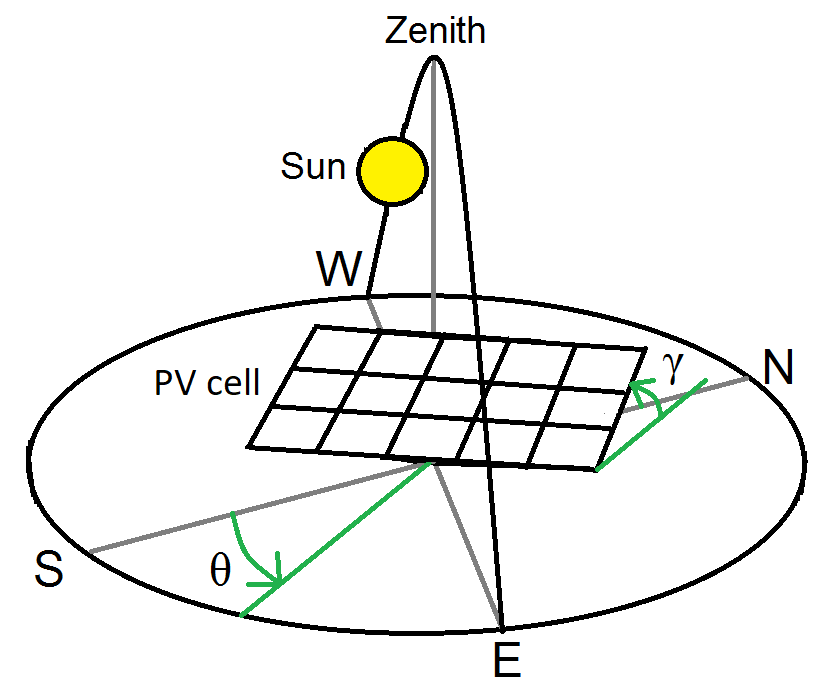
\includegraphics[width=0.6\textwidth]{pictures/nnnew}
\caption[Depiction of a PV cell installed with the orientation angle $\theta$ and inclination angle $\gamma$]{Depiction of a PV cell installed with the orientation angle $\theta=-30^{\mathrm{o}}$ and inclination angle $\gamma=20^{\mathrm{o}}$\label{angle}}
\end{figure}

The daily energy generation profile of a PV cell depends on the day of the year, the deployment location, the orientation angle $\theta$, and the inclination angle $\gamma$ of the PV cell.

The orientation and inclination angles of PV cells are usually fixed after the initial installation. Therefore, it is necessary to optimize the orientation and inclination angles of PV cells prior to the deployment. Without considering the energy consumption profile of the appliance, PV cells are deployed with default angles that are derived from the PV cell's geographic location as summarized in Table \ref{over}. The default inclination angle is set at a value similar to the latitude of the deployment area, and the default orientation angle is $0^{\mathrm{o}}$, and $180^{\mathrm{o}}$ in the northern, and southern hemispheres, respectively \cite{Solar_Cell}. Deploying PV cells with the default angles from Table \ref{over} guarantees that the PV cells harvest the most energy on a yearly timescale among all possible orientation and inclination angles. 





\begin{table}[H]
 \centering
\captionsetup{justification=centering}
\caption{\\ Default optimal orientation angle $\theta$ and inclination angle $\gamma$ for different locations \cite{Solar_Cell} \label{over}}
\label{overview}
\begin{tabularx}{\columnwidth}{@{}l*{2}{|C}Cc@{}}\toprule
\textbf{Location}					&  $\boldsymbol{\theta}$ 	&$\boldsymbol{\gamma}$ \\ \midrule
Northern hemisphere	& $0^{\mathrm{o}}$ 																&similar to the location's latitude						\\ 
Southern hemisphere	& $180^{\mathrm{o}}$ 															&similar to the location's latitude						\\ 
Equator							& any orientation angle &$0^{\mathrm{o}}$\\ \bottomrule
\end{tabularx}
\end{table}



This paragraph will investigate how the shape of the energy generation profile changes for different orientation angles on a daily timescale. 
Figure \ref{different_orientation_profiles} shows the daily energy generation profiles of southeast-oriented, south-oriented, and southwest-oriented PV cells, which are denoted by $G_{-45^{\mathrm{o}},1}(t)$, $G_{0^{\mathrm{o}},1}(t)$, and $G_{45^{\mathrm{o}},1}(t)$, respectively, for Greenwich (London, UK) during the summer. Orientating a PV cell eastwards (westwards) shifts the energy generation profile towards the morning (afternoon) hours in the northern hemisphere. The farther a PV cell is oriented away from the southern direction the less energy it harvests throughout the day. In other words, the more the energy generation profile peak is shifted away from noon the less energy is produced by the PV cell throughout the day. This tradeoff will be addressed in this thesis to determine the optimal orientation angle. 



\begin{figure}[H]
	\centering
		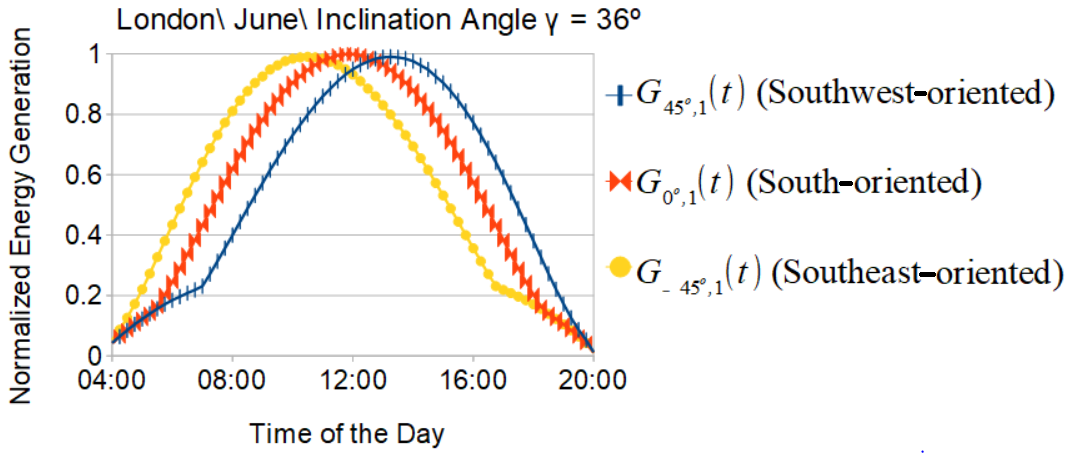
\includegraphics[width=1\columnwidth]{pictures/orien}
\caption{Effects of the orientation angle $\theta$ on the energy generation profile of the PV cell\label{different_orientation_profiles}}
\end{figure}

Optimizing the PV cell orientation angle is done on a daily timescale because it is a method to shift the energy generation peak from a surplus time (e.g. noon) to a deficit time (e.g. morning or afternoon), as seen in Figure \ref{different_orientation_profiles}. In contrast, optimizing the PV cell inclination angle is done on a yearly timescale because it is a method to shift the energy generation peak from a surplus season (e.g. summer) to a deficit season (e.g. winter). The focus of this thesis is to match the daily energy consumption profile of a BS with the daily energy generation profile of several PV cells. Hence, the orientation angles will be optimized in this thesis because the orientation angles affect the shape of the energy generation profile on a daily timescale. 




\section{Types of PV Cells\label{type_pv}}
PV cells can be classified into fixed, sun tracking, and adjustable PV cells (cf. \mbox{Figure \ref{ar}}). A fixed PV cell (cf. \mbox{Figure \ref{ar}(\subref{1})}) has fixed orientation and inclination angles which cannot be changed anymore after the initial installation. A single-axis sun tracking PV cell (cf. \mbox{Figure \ref{ar}(\subref{2})}) can mechanically track the sun throughout the day via adjusting the orientation angle. The single-axis sun tracking PV cell improves herein its daily energy yield compared with a fixed PV cell. A dual-axis sun tracking PV cell (cf. \mbox{Figure \ref{ar}(\subref{3})}) can mechanically track the sun throughout the day and the season, e.g., winter and summer, via adjusting both the orientation and inclination angles. The dual-axis sun tracking PV cell improves herein its yearly energy yield compared with a single-axis sun tracking PV cell. 


Despite the potentially higher energy yield of sun tracking PV cells than fixed PV cells, they are currently not widely deployed. The reasons are mainly the additional parts needed (e.g. axis motor), the higher maintenance (e.g. mechanical parts like the axis and the motor break more often than static parts), and the energy needed to operate the axis motor, which can be higher than the additional energy generated due to the sun tracking for some locations \cite{EKE20122665}. 


An adjustable PV cell (cf. \mbox{Figure \ref{ar}(\subref{4})}) requires an engineer to visit the site several times throughout the year to adjust the angles manually. Frequent (infrequent) adjustments of the angles will result in higher (lower) operational expenditure in combination with a higher (lower) energy yield of the PV cell. Due to the high wages in many countries, the increasing number of BSs in future cellular networks, and the problem that many BSs are difficult to access (e.g. on top of buildings or mountains), fixed PV cells are more suitable for powering BSs than adjustable PV cells. Hence, this thesis will focus on orientation angle optimization of fixed PV cells. Nonetheless, the derived optimization process in this thesis can equivalently be used to optimize the orientation angles of adjustable PV cells. For example, if the optimization method in this thesis is done on two days throughout the year (e.g. one day in winter, and one day in summer), the two derived optimal orientation angles can be altered every 6 months. The engineer should change the orientation angles of the adjustable PV cells during spring equinox and autumn equinox every year for this example. In general, fixed PV cells can be seen as a special case of an adjustable PV cell that does not require additional visits of engineers after its initial installation.





\begin{figure}[H]
\minipage{0.25\columnwidth}
  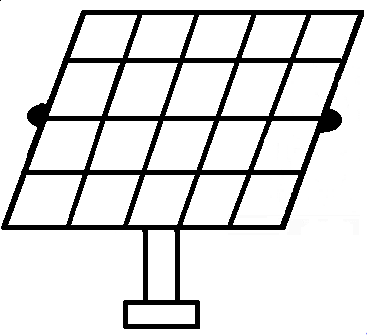
\includegraphics[width=\textwidth]{pictures/k1.png}
\subcaption{\label{1}}
\endminipage
\minipage{0.25\columnwidth}
  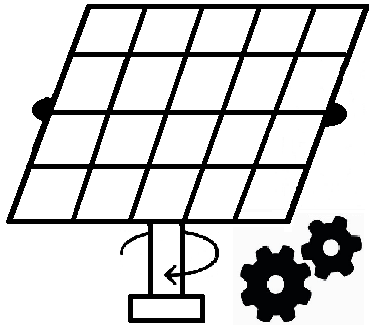
\includegraphics[width=\textwidth]{pictures/k2.png}
\subcaption{\label{2}}
\endminipage
\minipage{0.25\columnwidth}
  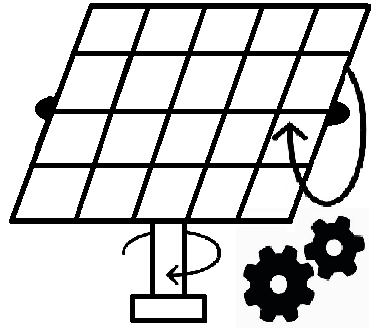
\includegraphics[width=\textwidth]{pictures/k3.png}
\subcaption{\label{3}}
\endminipage
\minipage{0.25\columnwidth}
  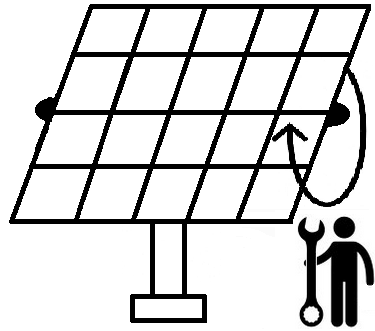
\includegraphics[width=\textwidth]{pictures/k5.png}
\subcaption{\label{4}}
\endminipage
\caption[Depiction of a fixed PV cell, a single-axis sun tracking PV cell, a dual-axis sun tracking PV cell, and an adjustable PV cell]{Depiction of a fixed PV cell (a), a single-axis sun tracking PV cell (b), a dual-axis sun tracking PV cell (c), and an adjustable PV cell (d) \label{ar}}
\end{figure}











\clearpage


\section{Motivation and Main Objective\label{Motivation_and_Objectives}}
In general, there is a mismatch between the daily energy generation profile of PV cells and the daily energy consumption profile of a BS, as seen in Figure \ref{bs}. The profiles in Figure \ref{bs} are given as an example in this paragraph. Many different types of energy generation profiles, and energy consumption profiles typical for PV cells, and typical for BSs will be evaluated in the following chapters, respectively. 

The objective of this thesis is to develop a method to shift the surplus energy (green color area in Figure \ref{bs}) to the deficit period (gray color area in Figure \ref{bs}). This thesis will derive a new methodology based on orientation angle optimization to adjust the solar energy supply to meet the energy demand of the
BS in the time domain (black arrow in Figure \ref{bs}). This is the main objective of this thesis and will be presented in Chapter \ref{Chapter_1}. 


\begin{figure}[H]
	\centering
		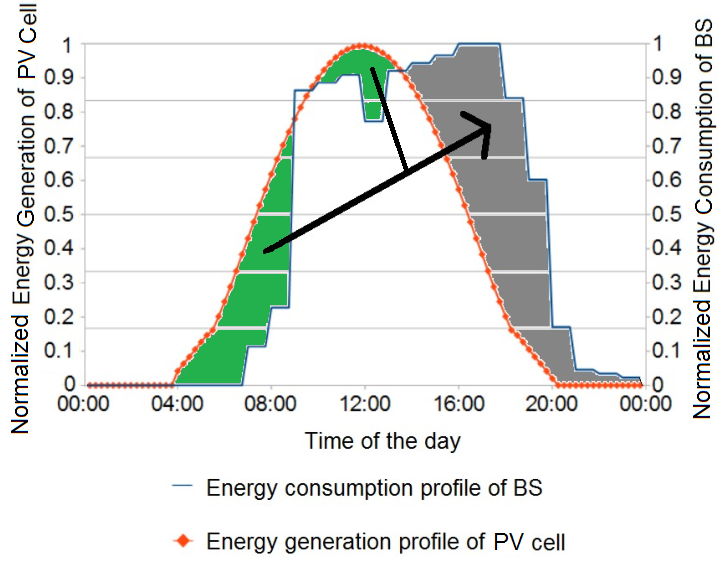
\includegraphics[width=0.7\columnwidth]{pictures/bs}
\caption{Example of an energy generation profile of a PV cell and an energy consumption profile of a BS to illustrate their mismatch\label{bs}}
\end{figure}



\clearpage
\section{Contributions\label{contributions}}
This section will summarize the main contributions of Chapter \ref{Chapter_1}, Chapter \ref{Chapter_2}, and Chapter \ref{Chapter_3}.


Contributions of Chapter \ref{Chapter_1}:

\begin{itemize}
\item Developing an algorithm to jointly optimize the orientation angles of several PV cells powering one BS. The algorithm achieves the best possible match between the energy generation profiles of the PV cells and the energy consumption profile of the BS. The proposed optimization algorithm only needs to be run a single time offline and the obtained optimal angles can be used for all solar-powered BSs with similar geographic locations and energy consumption profiles.
\item Deriving analytically the irradiance values on any randomly inclined and oriented PV cell. A horizontally-mounted PV cell is used as a baseline and its irradiance values have to be given to derive the irradiance values on any randomly inclined and oriented PV cell at the same location.
\item Identifying and discussing analytically to what extent the orientation angle $\theta$ shifts the energy generation profile away from noon if the PV cells are not south-oriented ($\theta \neq 0^\mathrm{o}$).  
\item Evaluating the effectiveness of the proposed orientation angle optimization on three different types of BS energy consumption profiles: constant traffic load profiles, business-area traffic load profiles, and residential-area traffic load profiles. The energy drawn from the main grid by the BS per day is used as the performance metric.
\item Giving recommendations on how many differently oriented PV cells should be deployed for a given energy consumption profile. To the best of my knowledge, this has never been investigated in the literature before.
\end{itemize}


Contributions of Chapter \ref{Chapter_2}:



\begin {itemize}
\item Developing a PV cell’s orientation angle optimization algorithm with Markov chain based battery model of a solar-powered BS with battery. The algorithm takes into account the battery capacity and the energy consumption profile of the BS. The number of user equipments (UEs) served by the BS throughout the day $\overline{S_{\mathrm{UE}}}(\theta)$ is used as the performance metric to identify the optimal orientation angle.
\item Verifying the accuracy of the proposed algorithm by showing that simulation trials converge based on the law of large numbers to 
the output $\overline{S_{\mathrm{UE}}}(\theta)$ of the proposed algorithm. 
\item Showing that the proposed algorithm (depends on the number of battery states) requires a shorter running time than the simulation trials (depends on the number of trials) for moderate battery state resolutions.
\item Investigating the dependency of the optimal PV cell orientation angle on the given battery capacity.
\end {itemize}


Contributions of Chapter \ref{Chapter_3}:


\begin{itemize}
\item  Developing an optimization algorithm that can be run once during the cellular network planning to determine what type of energy harvesters should be deployed to every BS in a cellular network. There are two different types of energy harvesters available for deployment which have anti-correlated energy generation profiles.
\item Taking into account the topology of the cellular network as well as the distance-dependent power loss in the distribution lines during the optimization.
\item Developing an optimization objective that maximizes the power that can be transmitted from surplus BSs to deficit BSs in the cellular network.
\item Comparing the proposed optimization algorithm with randomly deploying anti-correlated energy harvesters to the BSs. The effects of different numbers of BSs, different distribution line existence probabilities, different distribution line power loss coefficients, and different power surplus values are investigated. 
\end{itemize}





\clearpage
\section{Organization\label{Organization}}
This section will present the organization of the thesis in detail. Section \ref{back} gives a general overview of the developments and emerging problems in future cellular networks and how solar-powered BSs can alleviate these emerging issues. Section \ref{def_an} defines the orientation and inclination angles of the PV cells and provides a basic rule of thumb how these angles should be chosen based on the geographical location of the PV cell. This rule of thumb only maximizes the yearly energy output of the PV cell but it cannot take into account the energy consumption profile of the appliance. Section \ref{type_pv} justifies the focus on fixed PV cells with respect to other types of PV cells in this thesis. Section \ref{Motivation_and_Objectives}, Section \ref{contributions}, and Section \ref{Organization} present the main objectives, the contributions, and the organization of this thesis, respectively. Chapter \ref{Chapter_1}, Chapter \ref{Chapter_2}, and Chapter \ref{Chapter_3} are the main parts of this thesis and are based on my published papers. Each of the three chapters develops a system model to address and to evaluate a specific problem explained in more detail later. Guidelines and key findings are summarized at the end of each chapter.

Chapter \ref{Chapter_1} addresses the main objective of this thesis. It develops a methodology to jointly optimize the orientation angles of several PV cells at one BS so that the energy generation profile of the PV cells matches the energy consumption profile of the BS. The system model of this chapter is presented in Section \ref{system_1} and consists of an energy generation model, a ground-reflected irradiance model, a direct-beam irradiance model, a sky-diffuse irradiance model, an energy consumption model, and an objective function. Section \ref{analytical} evaluates analytically to what extent the orientation angle $\theta$ determines the position of the peak of the energy generation profile in the time domain. The numerical results and the key findings are presented in Section \ref{results}. Finally, the chapter is summarized in Section \ref{sum_Chapter_1}.



Chapter \ref{Chapter_2} extends the system model from Chapter \ref{Chapter_1} by adding a battery to the BS. The battery is modeled by a Markov chain. Section \ref{system_2} presents the system model of this chapter. Section \ref{jj} derives the PV cell's orientation angle optimization algorithm with Markov chain based battery model of a solar-powered BS with battery. Section \ref{see} introduces a simulation algorithm as a baseline for the comparison and evaluation of the proposed algorithm. Section \ref{results_system_2} discusses and presents numerical results. In more detail, Section \ref{n} investigates the running time of both algorithms. Section \ref{anna} verifies the accuracy of the proposed algorithm with simulation results.
Section \ref{new} shows the strong dependency of the optimal PV cell orientation angle on the battery capacity. Finally, the chapter is summarized in Section \ref{sum_Chapter_2}. 

Chapter \ref{Chapter_3} extends the previous system model to a multi-cell cellular network. There are now several BSs distributed in an area and some of them are connected by distribution lines to share the renewable energy among them. The problem investigated in this chapter is how energy harvesters with anti-correlated energy generation profiles should be deployed to every BS so that the renewable energy can be shared most efficiently in the multi-cell cellular network. Two PV cells that have significantly different orientation angles, such as east-oriented and west-oriented PV cells, are an example for energy harvesters with anti-correlated energy generation profiles. Section \ref{system_model_3} presents the system model of this chapter, which consists of the definition of the power surplus/deficit values, the derivation of the distance-dependent power loss in the distribution lines, and the definition of the topology of the cellular network. The objective function of this chapter is derived in Section \ref{MILPP_pres} and based on a mixed-integer linear programming problem (MILPP). Section \ref{numeric_results_system_3} presents the system performance improvements achieved by optimizing the deployment of the energy-harvesters with the MILPP in comparison with randomly deploying the energy harvesters. Finally, the chapter is summarized in Section \ref{sum_Chapter_3}.
 
Chapter \ref{conclusion} concludes the thesis by summarizing its achievements, highlighting future application areas, and outlining future work in this area. 
An appendix and a list of references are attached at the end of this thesis.









\clearpage
\chapter{PV Cell Orientation Angles Optimization for a Base Station Equipped with Several PV Cells\label{Chapter_1}}

\section{Literature Review: Orientation Angle Optimization}
Many papers in the literature map for a given PV cell its performance in a wide geographical area. The average yearly or daily energy output of the PV cell is used as the performance metric. For each geographical location in the investigated area, the latitude, the longitude, the altitude, the ambient temperature, the wind speed, the solar spectrum, and site-specific weather conditions are often used to determine the performance of the PV cell. Nonetheless, these papers do not optimize any of the parameters of the PV cell, such as the orientation angle, instead they derive a guideline for the best deployment area for the given PV cell type. For example, \cite{south_africa}, \cite{HuldThomas2010Mtpo} and \cite{ThomasHuld2015EPMP} derive comprehensive guides for PV cell deployment areas in South Africa, Europe, and Eurasia, respectively.  
In addition, geographic information systems (GISs) provide such guides for various geographical areas online, such as for the USA \cite{usa}, for Europe \cite{PVGIS}, and worldwide \cite{worldwide,worldwide2}. 



Most papers investigating differently oriented PV cells, such as \cite{ORDONEZ20102122}, have not actually optimized the PV cell angles but considered some deployment constraints, e.g., that the PV cells are mounted on residential rooftops, which predefine the PV cell angles. 

Other papers, such as \cite{VALLADARESRENDON2017458}, optimize the orientation of objects to increase or decrease the sun irradiance on the object. These objects do not have to be PV cells. For example, \cite{VALLADARESRENDON2017458} determines the optimal orientation of a building (no PV cells are deployed) so that less sun irradiance can enter the building through the windows. In climates with abundant sun irradiance, orientating the buildings so that less irradiance can enter the buildings through the windows reduces the need for cooling the buildings with air conditioning.


PV cell angle optimization for maximizing the total energy output of the PV cells has been done for Singapore in \cite{irradianceModels}, however, without considering the potential mismatch between the energy generation profile of the PV cells and the energy consumption profile of the appliance. This may result in service outage if the PV cells are the only energy source or additional expenditures if the energy deficit has to be compensated by using alternative energy sources. Different from \cite{irradianceModels}, the optimal PV cell orientation angles are derived in this thesis to match a given energy consumption profile rather than maximizing the total energy output of the PV cells. 

In \cite{Kemery2012OptimalPO}, the PV cell angle optimization considered the energy demand of the Ontario province of Canada, where the authors investigated orientation angles from $15^\mathrm{o}$ east of due south to $15^\mathrm{o}$ west of due south, i.e., $\theta\in[-15^{\mathrm{o}},15^{\mathrm{o}}]$. But propagation losses along the power lines among the widely-distributed PV cell installations were not included, which are significant factors when operating on a provincial scale \cite{8491374,my_con3}. Different from \cite{Kemery2012OptimalPO}, the optimal PV cell orientation angles are derived in the range from east ($\theta=-90^\mathrm{o}$) to west ($\theta=90^\mathrm{o}$) in this thesis.

The authors of \cite{CHATTOPADHYAY2017176} investigated five orientation angle settings (east, southeast, south, southwest, and west) and concluded that in some scenarios a mix of east-oriented and west-oriented PV cells and in other scenarios south-oriented PV cells reduce the needs for storage and backup from dispatchable energy sources in a fully renewable European power system. Because they adjusted the installed capacity of the PV cells for each angle configuration, such that the average power production of each PV cell remains the same, it is difficult to fairly judge if the reduced needs for storage and backup are a good trade-off for the increased installed capacity of PV cells. Different from \cite{CHATTOPADHYAY2017176}, the installed capacity of the PV cells is kept unchanged in this thesis. Hence, it is possible to fairly present the improvements caused by different PV cell orientation angles in this thesis.


Optimizing the PV cell inclination angle to power an isolated island was studied in \cite{7315106}, where the PV cell inclination angle was optimized on a yearly timescale. Because the PV cell inclination angle was optimized, the energy can be shifted on a yearly timescale, i.e., from a surplus season (e.g. summer) to a deficit season (e.g. winter), but the energy cannot be shifted on a daily timescale, i.e., from a surplus time (e.g. noon) to a deficit time (e.g. morning or afternoon) with the proposed method in \cite{7315106}.  



In my papers \cite{my,my2,my4}, I have been optimizing the PV cell orientation angle of one PV cell deployed at the BS to match the energy generation of this single PV cell with the energy consumption of a BS. Optimizing the PV cell orientation angle of several PV cells deployed at the BS to match the energy generation of the PV cells with the energy consumption of a BS has been studied in my paper \cite{sub}. Hence, my paper \cite{sub} is an extension to my previous papers \cite{my,my2,my4}. Chapter \ref{Chapter_1} of this thesis is based on \cite{sub}. In contrast to \cite{my,my2,my4}, \cite{sub} can investigate how the number of PV cells and the composition of differently oriented PV cells improve the match between the energy generation profile of the PV cells and the energy consumption profile of the BS.

\section{Contributions of Chapter \ref{Chapter_1}}
The contributions of Chapter \ref{Chapter_1} are summarized as follows:

\begin{itemize}
\item Developing an algorithm to jointly optimize the orientation angles of several PV cells powering one BS. The algorithm achieves the best possible match between the energy generation profiles of the PV cells and the energy consumption profile of the BS. The proposed optimization algorithm only needs to be run a single time offline and the obtained optimal angles can be used for all solar-powered BSs with similar geographic locations and energy consumption profiles.
\item Deriving analytically the irradiance values on any randomly inclined and oriented PV cell. A horizontally-mounted PV cell is used as a baseline and its irradiance values have to be given to derive the irradiance values on any randomly inclined and oriented PV cell at the same location.
\item Identifying and discussing analytically to what extent the orientation angle $\theta$ shifts the energy generation profile away from noon if the PV cells are not south-oriented ($\theta \neq 0^\mathrm{o}$).  
\item Evaluating the effectiveness of the proposed orientation angle optimization on three different types of BS energy consumption profiles: constant traffic load profiles, business-area traffic load profiles, and residential-area traffic load profiles. The energy drawn from the main grid by the BS per day is used as the performance metric.
\item Giving recommendations on how many differently oriented PV cells should be deployed for a given energy consumption profile. To the best of my knowledge, this has never been investigated in the literature before.
\end{itemize}



\section{System Model 1 - Several PV Cells Powering One BS\label{system_1}}
Figure \ref{ene} depicts the system model 1 considered in Chapter \ref{Chapter_1}. The energy generation part consists of $N$ identical PV cells, denoted by PV cell 1, PV cell 2, ..., and PV cell $N$, $N \in \mathbb{N}$. The energy consumption part consists of a BS. The total surface area of all $N$ PV cells is $A$. Each PV cell has a surface area of $\frac{A}{N}$. The day is divided into $T$ time steps, $T\in\mathbb{N}$. The index of a time step is denoted by $t$, $t \in \{1,...,T\}$.
The BS uses the energy generated by the $N$ PV cells, denoted by $G(t)$, to support its energy consumption $C(t)$ at every time step $t$. 
If there is an energy deficit, i.e., $C(t)-G(t)>0$, the BS draws the remaining energy from the main grid at time step $t$. If there is an energy surplus, i.e., $C(t)-G(t)<0$, the surplus energy is wasted at time step $t$ or fed to the grid\footnote{There are no feed-in tariffs considered in this thesis because I want to incentify that the generated energy is used locally. Large amounts of intermittent generated energy which is fed into the grid often causes unbalancing issues, and voltage drops in the grid or in the worst-case scenario a black out. Matching the energy generation profile with the energy consumption profile on-site at a BS reduces therefore the stress on the power grid. This assumption is justified because most power grids nowadays are still designed for one-directional energy flow from a few large-scale centralized energy generators, such as coal power plants or nuclear power plants, to many small-scale energy consumers, such as domestic households or BSs. Current power grid infrastructure is often not assigned to accommodate huge amounts of energy flow in opposite direction and to redistribute such intermittent generated energy sufficiently without causing grid instability or jeopardizing the reliability of the power grid. Even if surplus energy can be sold to the grid, the system model 1 aims to match the energy generation profile with the energy consumption profile on-site at a BS, which is more cost-effective for the BS/ PV cells owner than wasting the surplus energy or selling the surplus energy to the grid for redistribution. Grid  operators always sell energy at a higher price than they buy it.}


The optimization object in the system model 1 is to minimize the amount of energy that has to be drawn from the main grid by the BS on a daily time scale. The energy drawn from the main grid can only be altered by choosing different orientation angles $\theta_1$, ..., and $\theta_N$ for PV cell 1, ..., and PV cell $N$, respectively. All the other parameters of the system, including the inclination angles of all $N$ PV cells, are fixed. In this thesis, the system is located in Greenwich (London, UK) as example, i.e., the Latitude $lat$, and the Longitude $lon$ are fixed to $51.4767^{\mathrm{o}}$ North, and $0.0003^{\mathrm{o}}$ West, respectively, but the analysis can be applied to other locations as well. Hence, all formulas in this thesis are given for a location in the northern hemisphere.


\begin{figure}[H]
\centering
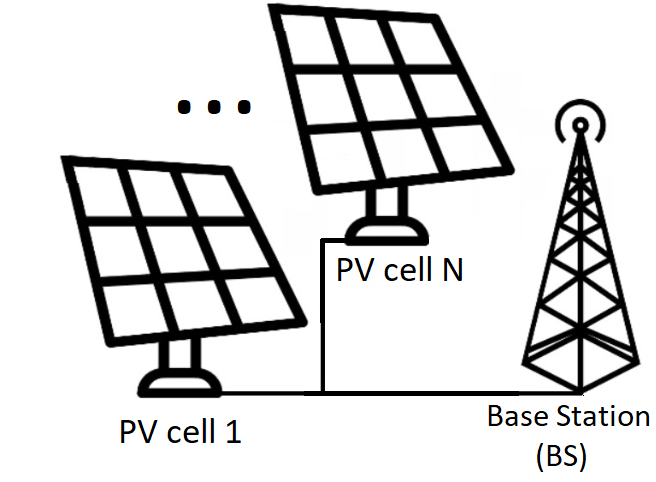
\includegraphics[width=0.6\columnwidth]{pictures/SystemSetup}
\caption{Illustration of system model 1\label{ene}}
\end{figure}

\subsection{Energy Generation of a PV Cell\label{gen}}

A horizontally-mounted PV cell in Greenwich (London, UK) is used as the baseline. From this baseline, a method will be developed to calculate the energy generated by a PV cell at the same location but installed with any orientation angle $\theta \in [-90^{\mathrm{o}},90^{\mathrm{o}}]$ and any inclination angle $\gamma\in[0,90^\mathrm{o}]$. The time is modeled in discrete time steps denoted by the time step index $t$, $t \in \{1,...,T\}$, hence all variables dependent on $t$ are discrete. The global horizontal irradiance $GHI_t$, the diffuse horizontal irradiance $DHI_t$, and the direct normal irradiance $DNI_t$ for a horizontally-mounted PV cell in Greenwich (London, UK) are obtained from the PVGIS database (cf. Figure \ref{PVGIS_datasheet}) for every time step $t$. Hence, $GHI_t$, $DHI_t$, and $DNI_t$, are considered given values for every time step $t$ and can be used throughout the thesis. 

\begin{figure}[H]
	\centering
		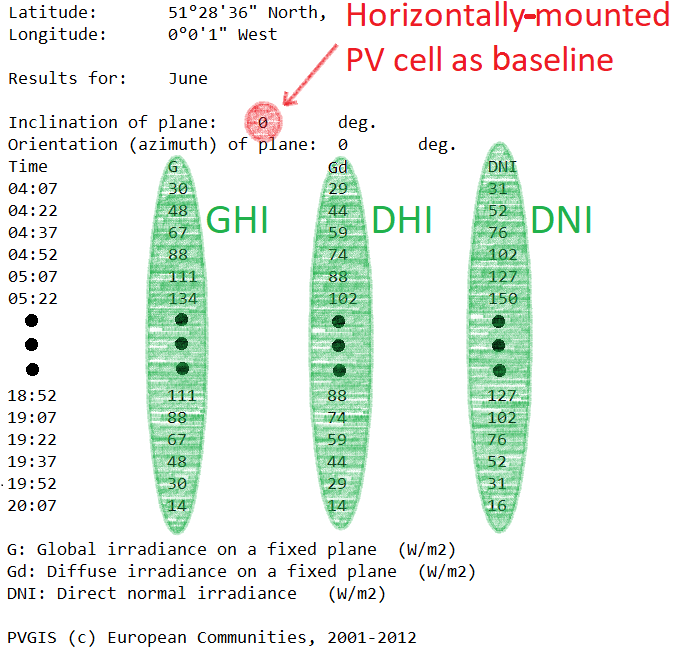
\includegraphics[width=0.7\columnwidth]{pictures/Greenwich5}
\caption[PVGIS data sheet]{PVGIS data sheet from \cite{PVGIS}\label{PVGIS_datasheet}}
\end{figure}

 
The energy generated by one PV cell installed with orientation angle $\theta$ and surface area $\frac{A}{N}$ is denote by $G^{\text{original}}_{\theta,N}(t)$ and can be calculated by \cite{add}\footnote{The total irradiance received by the PV cell $I_{\theta}(t)$ adjusted for angle of incidence losses inside of the PV cell module, for soiling, e.g., dust or snow, for temporal losses, and for spectral mismatch is called the effective irradiance (irradiance that is “available” to the PV cell for power conversion). The material covering a cell in a PV module, e.g., glass, and encapsulate, causes due to reflection and absorption different losses at different angles of incidence. It is out of the scope of this thesis to calculate any internal energy losses of the PV cell due to its structure or composition. Therefore, it is assumed for simplicity that the total irradiance received by the PV cell $I_{\theta}(t)$ is the effective irradiance available by the PV cell for conversion in this thesis.} as follows:

\begin{equation}\label{normalization}
G^{\text{original}}_{\theta,N}(t)=I_{\theta}(t) \cdot \eta \cdot \frac{A}{N} \cdot \tau,
\end{equation}
where $I_{\theta}(t)$ is the irradiance received by the PV cell, $\eta$ is the energy conversion efficiency, $\frac{A}{N}$ is the surface area of the PV cell, and $\tau$ is the duration of one time step.

To facilitate a fair comparison in Section \ref{results}, all energy generation values are normalized with respect to a south-orientated PV cell in Greenwich at noon with surface area $A$, and inclination angle $\gamma=36^{\mathrm{o}}$ (optimal inclination angle for Greenwich (London, UK) in summer). Among all orientation angle settings and among all time steps throughout the day, the peak energy generation occurs during noon when all available PV cells are south-oriented in Greenwich. This is because Greenwich is located on the reference meridian of its time zone. The time step $t=\frac{T}{2}$ is noon. Because a south-orientated PV cell in Greenwich has its peak energy generation at noon, i.e., $I_{0^{\mathrm{o}}}\big(\frac{T}{2}\big)\geq I_{0^{\mathrm{o}}}\big(t\big)\quad \forall t\in\{1,...,T\}$, the peak irradiance value at noon, i.e, $614[\frac{W}{m^2}]=I_{0^{\mathrm{o}}}\big(\frac{T}{2}\big)$, is used as normalization factor in this thesis. The peak irradiance value is derived from \cite{PVGIS} by downloading the data sheet for a south-oriented PV cell in Greenwhich with  inclination angle $\gamma=36^{\mathrm{o}}$. The normalization factor $614$ has the effect that exactly 1 unit of normalized energy is generated by the south-oriented PV cell at noon after normalization. This normalization is done for convenience. Any normalization factor can be used but normalization the peak energy generation to 1 unit of energy is convenient when representing the results in graphs. Other locations than Greenwich (London, UK) will have to use their respective normalization factor and their respective optimal inclination angle. Appendix A will do the normalization process step by step for a better understanding.


Hence, $G_{\theta,N}(t)$ is the normalized energy generated by one PV cell out of the $N$ PV cells installed with orientation angle $\theta$ and can be calculated by

\begin{equation}\label{norma}
G_{\theta,N}(t)=\frac{G_{\theta,N}^{\text{original}}(t)}{G^{\text{original}}_{0^{\mathrm{o}},1}\big(\frac{T}{2}\big)}=\frac{I_{\theta}(t)}{I_{0^{\mathrm{o}}}\big(\frac{T}{2}\big)\cdot N}= \frac{I_{\theta}(t)}{614\cdot N}.
\end{equation}



The normalized energy generated by $N$ PV cells, denoted by $G_{(\theta_1, ..., \theta_N)}(t)$, is calculated as follows:
\begin{equation}\label{nor}
G_{(\theta_1, ..., \theta_N)}(t)=\sum_{i=1}^N G_{\theta_i,N}(t).
\end{equation}

As a result, if all $N$ PV cells are oriented to the south, they generate exactly 1 unit of energy at noon, i.e., $G_{(\theta_1, ..., \theta_N)}\big(\frac{T}{2}\big)=G_{(0^{\mathrm{o}}, ...,0^{\mathrm{o}})}\big(\frac{T}{2}\big)=1$.



The irradiance $I_{\theta}(t)$ received by one PV cell installed with orientation angle $\theta$ at time step $t$ can be calculated by \cite{Solar_Cell_3irradiance} as follows:


\begin{equation}\label{I1}
I_{\theta}(t)=I_{b_\theta}(t)+I_{d_\theta}(t)+I_{g}(t),
\end{equation}
where $I_{b_\theta}(t)$ is the direct-beam component, $I_{d_\theta}(t)$ is the sky-diffuse component, and $I_{g}(t)$ is the ground-reflected component. Figure \ref{3irradiances} shows the three components graphically. The three irradiance components are investigated in the next three sections separately.

\begin{figure}[H]
	\centering
		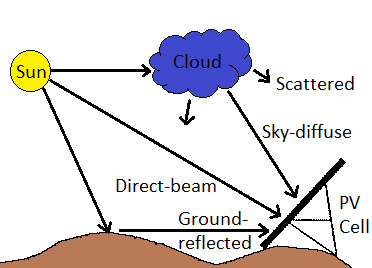
\includegraphics[width=0.6\columnwidth]{pictures/3irradiances}
\caption{Irradiance model\label{3irradiances}}
\end{figure}



\subsection{Ground-reflected Irradiance \texorpdfstring{$I_g(t)$}{I\_g(t)}}\label{ground_reflected_component}

The ground-reflected irradiance $I_{g}(t)$ is independent of the orientation angle $\theta$ and can be calculated by \cite{Solar_Cell_albedo_plus_ground_reflected_irradiance} as follows:


\begin{equation}\label{I3}
I_{g}(t)= GHI_t \cdot \alpha \cdot \frac{1-\cos(\gamma)}{2},
\end{equation}
where $\alpha\in[0,1]$ is the albedo of the ground. The albedo is dimensionless and measures the amount of sunlight that a surface reflects. A black body that absorbs all sunlight has an albedo value of $0$. A body that reflects all sunlight has an albedo value of $1$. For example, snow has a high albedo and hence, appears bright. Trees have a low albedo and hence, appear dark.



\subsection{Direct-beam Irradiance \texorpdfstring{$I_{b_\theta}(t)$}{I\_{b\_{\{theta\}}}(t)}}\label{direct_beam_component}
The direct-beam irradiance $I_{b_\theta}(t)$ depends on the orientation angle $\theta$ and can be calculated by \cite{Solar_Cell_3irradiance} as follows:


\begin{equation}\label{I4}
I_{b_\theta}(t)=DNI_t \cdot  \max(0,\cos(AOI_{\theta}(t))),
\end{equation}
where $AOI_{\theta}(t)$ is the angle of incidence at time step $t$.

It is important to include the $\max$ in (\ref{I4}) to model that no energy can be harvest if the PV cell is illuminated from the back, i.e., $AOI_{\theta}(t)>90^\mathrm{o}$. For example, if the PV cell is oriented to the east then $AOI_{\theta}(t)$ will be greater than $90^\mathrm{o}$ in the evening. Hence, $\cos(AOI_{\theta}(t))$ will be smaller than $0$. This will result in a negative irradiance value $I_{b_\theta}(t)$ during the evening, which makes no sense. As a result, the $\max$ in (\ref{I4}) is necessary.

The angle of incidence $AOI_{\theta}(t)$ is the angle between the line that points to the sun and the normal vector to the PV cell panel (cf. Figure \ref{AOI}). $AOI_{\theta}(t)$ can be calculated by \cite{Solar_Cell_declination_inclination_angle} as follows:

\begin{align}
\cos(AOI_{\theta}(t))= &\quad \textcolor{SeaBlue}{+ \sin(\delta_d) \sin(lat) \cos(\gamma)} \nonumber \\
					 &\quad \textcolor{SeaBlue}{+ \cos(\delta_d) \cos(lat) \cos(\gamma) \cos(\omega_t)} \nonumber \\
			   	 &\quad \textcolor{Orange8}{+ \cos(\delta_d) \sin(\gamma) \sin(\omega_t)} \!\!\enskip \textcolor{red!70}{ \sin(\theta)} \nonumber \\
					 &\quad \textcolor{Gray7}{- \sin(\delta_d) \cos(lat) \sin(\gamma)} \!\!\enskip \textcolor{red}{ \cos(\theta)} \nonumber \\
					 &\quad \textcolor{Gray7}{+ \cos(\delta_d) \sin(lat) \sin(\gamma) \cos(\omega_t)} \!\!\enskip \textcolor{red}{ \cos(\theta)} \label{allgemein_AOI}\\
					= &\quad \textcolor{SeaBlue}{a_t} +\textcolor{Orange8}{b_t} \textcolor{red!70}{\sin(\theta)} + \textcolor{Gray7}{c_t} \textcolor{red}{\cos(\theta)}, \text{ with}\nonumber 
\end{align}




\begin{align}
\textcolor{SeaBlue}{a_t}=&\quad \textcolor{SeaBlue}{+ \sin(\delta_d) \sin(lat) \cos(\gamma)}\nonumber  \\
					               &\quad \textcolor{SeaBlue}{+ \cos(\delta_d) \cos(lat) \cos(\gamma) \cos(\omega_t)}, \label{a_t}\\
\textcolor{Orange8}{b_t}=&\quad \textcolor{Orange8}{+ \cos(\delta_d) \sin(\gamma) \sin(\omega_t)} \label{b_t},\\
  \textcolor{Gray7}{c_t}=&\quad \textcolor{Gray7}{- \sin(\delta_d) \cos(lat) \sin(\gamma)} \nonumber  \\
					               &\quad \textcolor{Gray7}{+ \cos(\delta_d) \sin(lat) \sin(\gamma) \cos(\omega_t)}, \label{c_t}
\end{align}
where $lat$ is the latitude of the deployment area, $\delta_d$ is the declination angle, and $\omega_t$ is the hour angle at time step $t$. $a_t$, $b_t$, and $c_t$ include the parts that are independent of $\theta$, are multiplied by $\sin(\theta)$, and are multiplied by $\cos(\theta)$, respectively.
\begin{figure} [H]
	\centering
		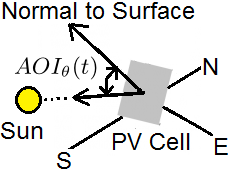
\includegraphics[width=0.3\textwidth]{pictures/AOI2}
		\caption{Definition of the angle of incidence $AOI_{\theta}(t)$\label{AOI}}
\end{figure}
The declination angle $\delta_d$ can be calculated by \cite{Solar_Cell_declination} as follows:


\begin{equation} \label{delta}
\delta_d=23.45^\mathrm{o} \cdot \sin\left(\frac{360}{365} (d+284)\right),
\end{equation}


where $d$ is the day of the year with $1^{\mathrm{st}}$ of January as $d = 1$.

The declination angle models the different seasons (cf. Figure \ref{decli}). $23.45^{\mathrm{o}}$ is the axial tilt of the earth.


\begin{figure}[H]
	\centering
		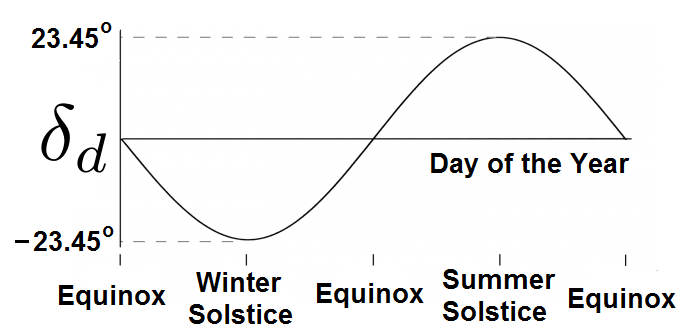
\includegraphics[width=0.6\columnwidth]{pictures/decli}
\caption{Declination angle $\delta_d$ throughout the year\label{decli}}
\end{figure}


The hour angle $\omega_t$ is defined as the angle between the meridian that intersects with the line that points to the sun and the meridian containing the observer (cf. Figure \ref{hour_angle}). 
The hour angle $\omega_t$ is depicted for Greenwich (London, UK) in Figure \ref{hour_angle_graph}. Because Greenwich (London, UK) is located on the reference meridian of its time zone, the straight line in Figure \ref{hour_angle_graph} intersects the x-axis at noon\footnote{The hour angles $\omega_t$ of locations that are not on their reference meridian of their time zone can be depicted by a straight line as well which is shifted along the x-axis. The formula to calculate the x-axis shift is given in \cite{Solar_Cell_hour_angle}.}. $\omega_t$ has a period of 24 hours and ranges from $-180^{\mathrm{o}}$ to $180^{\mathrm{o}}$.




\begin{figure} [H]
	\centering
		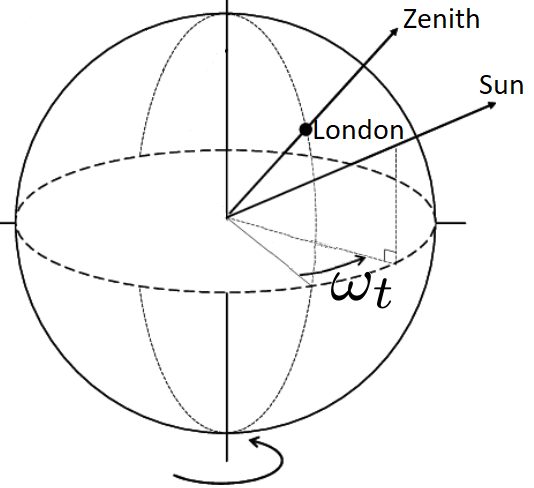
\includegraphics[width=0.3\textwidth]{pictures/hour_angle}
		\caption{Definition of the hour angle $\omega_t$\label{hour_angle}}
\end{figure}



\begin{figure}[H]
	\centering
		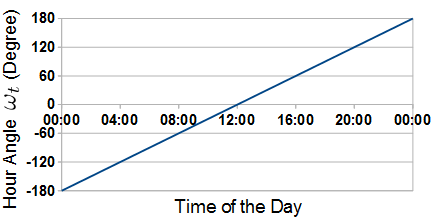
\includegraphics[width=0.6\columnwidth]{pictures/hour_angle_graph}
\caption{Hour angle $\omega_t$ throughout the day of a PV cell located on the reference meridian of its time zone \label{hour_angle_graph}}
\end{figure}


\subsection{Sky-diffuse Irradiance \texorpdfstring{$I_{d_\theta}(t)$}{I\_{d\_\{theta\}}(t)}}\label{sky_diffuse_component}
The sky-diffuse irradiance $I_{d_\theta}(t)$ is derived from the Reindl model\footnote{The difference between different irradiance models are usually in the way they model the sky-diffuse irradiance \cite{different_irradiance_model,DemainColienne2013Eodm,BertrandCdric2015Eodm}. The simplest and most commonly used model is the Liu and Jordan model, which assumes an isotropic diffuse sky \cite{irradianceModels}. In other words, the diffuse-sky irradiance is uniform across the sky and hence, the diffuse-sky irradiance is independent of the orientation angle $\theta$. The more advanced Reindl model is used in this thesis \cite{GueymardChristianA.2009Daiu}, which breaks the diffuse-sky irradiance into three separate parts: the isotropic component, the circumsolar component, and the horizon brightening component. The first component is the same as the Liu and Jordan model, while the other components are small correction terms. The circumsolar component dependents on the orientation angle $\theta$.} \cite{reindl,diffuse} as follows:

\footnotesize


\begin{align}\label{reindl}
I_{d_\theta}(t)=&\underbrace{DHI_t\cdot\vphantom{\sqrt(\frac{(X)^x_x}{(X)^x_x})}A_t\cdot \frac{\max(0,\cos(AOI_{\theta}(t)))}{\cos(\zeta_t)}}_{\text{Circumsolar Component}}+\underbrace{DHI_t\cdot(1-A_t)\cdot\frac{1+\cos(\gamma)}{2}}_{\text{Isotropic Component}}+\nonumber\\
&\underbrace{DHI_t\cdot(1-A_t)\cdot\frac{1+\cos(\gamma)}{2} \cdot\sqrt{\frac{DNI_t\cdot \cos(\zeta_t)}{GHI_t}}\sin^3\bigg(\frac{\gamma}{2}\bigg)}_{\text{Horizon Brightening Component}}=\nonumber\\
DHI_t\bigg[\vphantom{\sqrt(\frac{(X)^x_x}{(X)^x_x})}&A_t\cdot \frac{\max(0,\cos(AOI_{\theta}(t)))}{\cos(\zeta_t)}+(1-A_t)\cdot\frac{1+\cos(\gamma)}{2}\cdot\bigg(\vphantom{\sqrt(\frac{(X)^x_x}{(X)^x_x})}1+\sqrt{\frac{DNI_t\cdot \cos(\zeta_t)}{GHI_t}}\sin^3\bigg(\frac{\gamma}{2}\bigg)\bigg)\bigg],\nonumber\\
\end{align}
\normalsize
where $A_t$ is the anisotropy index, and $\zeta_t$ is the solar zenith angle. The Reindl model breaks the diffuse-sky irradiance into three separate parts: the isotropic component, the circumsolar component, and the horizon brightening component (cf. (\ref{reindl})). The circumsolar component depends on the orientation angle $\theta$. The isotropic component, and the horizon brightening component do not depend on the orientation angle $\theta$.



The solar zenith angle $\zeta_t$ can be calculated by \cite{zenith_angle} as follows:


\begin{equation}\label{zenith}
\cos(\zeta_t)=\sin(lat)\sin(\delta_d)+\cos(lat)\cos(\delta_d)\cos(\omega_t).
\end{equation}


The anisotropy index $A_t$ of time step $t$ can be calculated by \cite{reindl} as follows:


\begin{equation} \label{At}
A_t=\frac{DNI_t}{E_d},
\end{equation}

\noindent
where $E_d$ is the extraterrestrial radiation. It can be calculated by \cite{Ea} as follows:


\begin{equation}\label{extra}
E_d=E_{\mathrm{con}}\cdot \bigg(\frac{\overline{r}}{r_d}\bigg)^2=E_{\mathrm{con}}\cdot\bigg(1+0.033 \cdot \cos \bigg(\frac{360 \cdot d}{365}\bigg)\bigg),
\end{equation}
where $E_{\mathrm{con}}$ is the solar constant set at $1367 \frac{\mathrm{W}}{\mathrm{m}^2}$ \cite{Solar_Cell_declination_inclination_angle}, $\overline{r}$ is the mean sun-earth distance also called $1$ astronomical unit ($1$ AU), $r_d$ is the actual sun-earth distance, which depends on the day of the year, and $d$ is the day of the year with $1^{\mathrm{st}}$ of January as $d = 1$.




\subsection{Energy Consumption of a BS\label{consumption}}


$C^{\text{original}}(t)$ is the original energy consumption by the BS during time step $t$ ($\tau$ is the duration of one time step) and $C(t)$ is the normalized energy consumption by the BS at time step $t$ and can be calculated by

\begin{equation}
C(t)=\frac{C^{\text{original}}(t)}{G^{\text{original}}_{0^{\mathrm{o}},1}\big(\frac{T}{2}\big)},
\end{equation}

where $G^{\text{original}}_{0^{\mathrm{o}},1}\big(\frac{T}{2}\big)$ is the peak energy generation of the PV cells if they are all south-oriented at noon.
A practical example is given in Appendix A to show step by step the process of normalization. 

$C(t)$ consists of a load-dependent part and a load-independent part. Three different load scenarios are investigated: a BS deployed with constant traffic load $C_{\mathrm{con}}(t)$, with business-area traffic load $C_{\mathrm{bus}}(t)$, and with residential-area traffic load $C_{\mathrm{res}}(t)$ (cf. Figure \ref{all_consumption_profiles}). Three different example energy consumption profiles are given to show the composition of C(t) into a load-dependent part and a load-independent part as follows:

\begin{align}
&C(t)=\underbrace{C_{\mathrm{con}}(t)}_{\text{load-dependent part}} + \underbrace{1}_{\text{load-independent part}}\\
&C(t)=\underbrace{C_{\mathrm{bus}}(t)}_{\text{load-dependent part}} + \underbrace{0.2}_{\text{load-independent part}}\\
&C(t)=\underbrace{C_{\mathrm{res}}(t)}_{\text{load-dependent part}} + \underbrace{0.7}_{\text{load-independent part}}.
\end{align}

The load-dependent part of the energy consumption profile determines the shape of the energy consumption profile, i.e., whether there is one significant peak in the profile, or several significant peaks in the profile or a very flat profile without any peaks.

The exact values for $C_{\mathrm{con}}(t)$, $C_{\mathrm{bus}}(t)$, and $C_{\mathrm{res}}(t)$ are given in Appendix B "Input File (Load Profiles)" for all time steps $t\in\{1,...,T\}$ as well as in Figure \ref{all_consumption_profiles}.
It can be observed that the traffic load in a business area ($C_{\mathrm{bus}}(t)$) is significantly higher during business hours than the rest of the day, while it drops a bit during lunch hours. Hence, there is one significant peak in the business area traffic load profile during afternoon hours. The traffic load in a residential area ($C_{\mathrm{res}}(t)$) is anti-correlated to the traffic load in a business area because it is higher during times when people are usually not working with its peak during late evening. This profile has peaks in the morning as well as in the evening.




\begin{figure}[H]
	\centering
		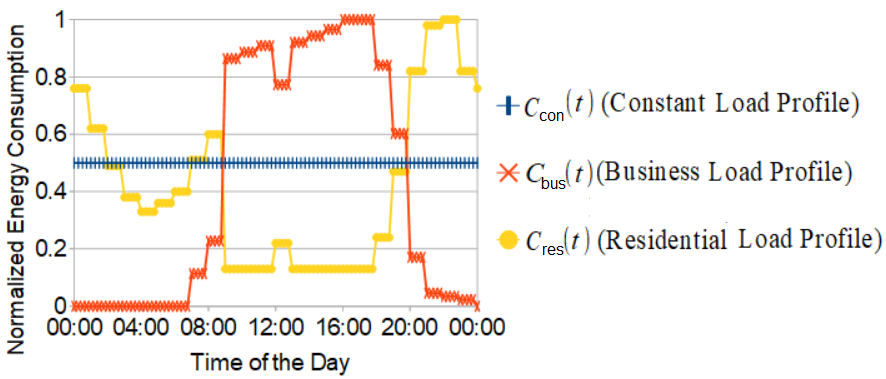
\includegraphics[width=0.8\columnwidth]{pictures/all_consumption_profiles2}
\caption[Constant traffic load profile, business traffic load profile, and residential traffic load profile throughout the day]{Constant traffic load profile, business traffic load profile, and residential traffic load profile throughout the day. Data source: \cite{load}\label{all_consumption_profiles}}
\end{figure}

For each of the three different load scenarios, I want to investigate how the relationship between the energy generation profile and the energy consumption profile affects the outcome of the orientation angles optimization. Therefore, I choose different values for the load-independent part of the energy consumption so that I have a case study in which the energy generation is significantly greater than the energy consumption ($G>>C$), the energy generation is slightly greater than the energy consumption ($G>C$), the energy generation is slightly smaller than the energy consumption ($G<C$), and the energy generation is significantly smaller than the energy consumption ($G<<C$). Figures \ref{constant_allgemein} - \ref{residential_allgemein} show all energy consumption profiles $C(t)$ which will be numerically investigated in section \ref{results}. The energy consumption profiles with the highest load-independent part in each figure belongs to the category $G<<C$. The energy consumption profiles with the lowest load-independent part in each figure belongs to the category $G>>C$.



To see the relationships between the energy consumption profiles $C(t)$ and the energy generation profiles $G(t)$, the combined energy generation profile of two south-oriented PV cells $G_{(0^\mathrm{o},0^\mathrm{o})}(t)$ as well as the combined energy generation profile of an east-oriented PV cell with a west-oriented PV cell $G_{(-90^\mathrm{o},90^\mathrm{o})}(t)$ are shown. 



\begin{figure}[H]
	\centering
		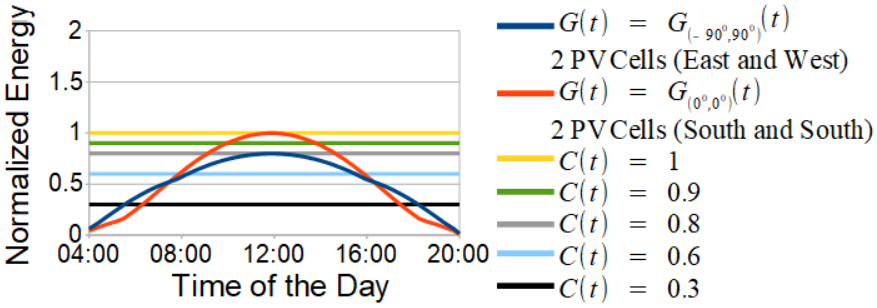
\includegraphics[width=1\columnwidth]{pictures/constant_allgemein3}
\caption{Energy consumption profiles with constant traffic load and energy generation profiles of 2 PV cells\label{constant_allgemein}}
\end{figure}


\begin{figure}[H]
	\centering
		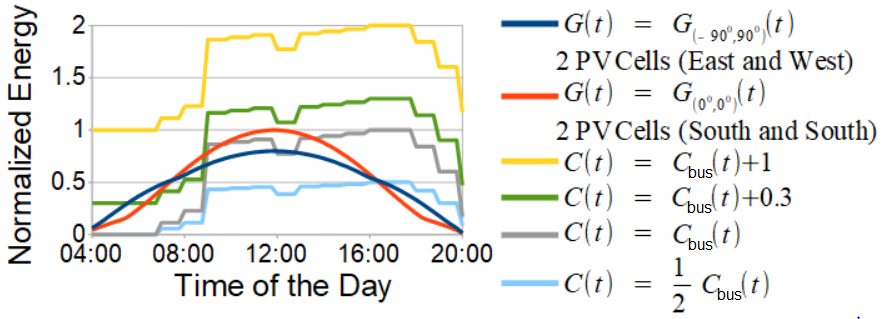
\includegraphics[width=1\columnwidth]{pictures/business_allgemein3}
\caption{Energy consumption profiles with business-area traffic load and energy generation profiles of 2 PV cells\label{business_allgemein}}
\end{figure}

\begin{figure}[H]
	\centering
		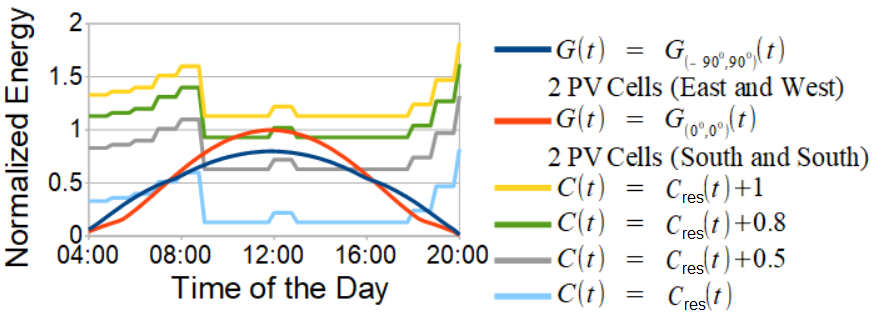
\includegraphics[width=1\columnwidth]{pictures/residential_allgemein3}
\caption{Energy consumption profiles with residential-area traffic load and energy generation profiles of 2 PV cells\label{residential_allgemein}}
\end{figure}




\subsection{Problem Formulation \label{generalization}}
The optimization objective is to minimize the normalized energy drawn from the main grid $f(\theta_1, ..., \theta_N)$ by the BS throughout the day which is defined in (\ref{optimization_objective}). The optimization problem is formulated as follows:

\begin{align}
f(\theta_1, ..., \theta_N)&=\sum_{t=1}^T \max\{0, C(t)-G_{(\theta_1, ..., \theta_N)}(t)\} \label{optimization_objective}\\
(\theta_1^*, ..., \theta_N^*)&=\arg \underset{(\theta_1, ..., \theta_N)}{\min}f(\theta_1, ..., \theta_N) \label{optimization_objective1},
\end{align}
where $(\theta_1^*, ..., \theta_N^*)$ are the optimal orientation angles for the $N$ PV cells.




Because surplus energy is wasted or fed to the grid with no feed-in tariff in the system model 1, the maximum out of  $0$ and $C(t) - G_{(\theta_1, ..., \theta_N)}(t)$ has to be taken in (\ref{optimization_objective}). It is assumed that energy can be bought from the grid at a fixed price throughout the day (flat rates). Hence, the objective function is to minimize the accumulated energy deficit throughout the day in (\ref{optimization_objective})-(\ref{optimization_objective1}). $f(\theta_1, ..., \theta_N)$ is transformed in (\ref{be}) - (\ref{intermit}). Eq. (\ref{intermit}) is used in Appendix B.




\begin{align}
f(&\theta_1, ..., \theta_N)=\sum_{t=1}^T \max\left\{0, C(t)-\sum_{n=1}^N G_{\theta_n,N}(t)\right\}\label{be}\\
&= \sum_{t=1}^T \max\bigg\{0, \underbrace{C(t)-\frac{I_{g}(t)}{614}}_{I_{\text{fix}}(t)}-\sum_{n=1}^N \frac{I_{b_{\theta_n}}(t)+I_{d_{\theta_n}}(t)}{{614}\cdot N}\bigg\}\\
&= \sum_{t=1}^T \max\bigg\{0,I_{\text{fix}}(t)-\sum_{n=1}^N \frac{I_{b_{\theta_n}}(t)+I_{d_{\theta_n}}(t)}{{614}\cdot N}\bigg\}\label{intermit}
\end{align}


The gain $\Delta_n$ of adding the $n^{\mathrm{th}}$ PV cell with optimal orientation angle $\theta_n^*$ to the system model 1 is defined as follows:


\begin{equation} \label{Delta_n}
\Delta_n=f(\theta_1^*,...,\theta_{n-1}^*)-f(\theta_1^*,...,\theta_n^*),\quad n\in \{2, ..., N\}.
\end{equation}


The gain of adding the first PV cell with optimal orientation angle $\theta_1^*$ to the system model 1 is defined as follows:

\begin{equation}\label{Delta_1}
\Delta_1=f(0^\mathrm{o})-f(\theta_1^*).
\end{equation}


A positive (negative) $\Delta_n$ value represents an improvement (deterioration) in performance of the system if the $n^{\mathrm{th}}$ PV cell is added, $n\in\{1, ..., N\}$.

\section{Analytical Insights obtained from Section \ref{system_1}\label{analytical}}
This section identifies and discusses analytically to what extent the orientation angle $\theta$ shifts the energy generation profile away from noon if the PV cells are not south-oriented ($\theta \neq 0^\mathrm{o}$). The direct-beam irradiance $I_{b_\theta}(t)$ and the sky-diffuse irradiance  $I_{d_\theta}(t)$ depend on $\theta$. Nonetheless, because the
main component of the sky-diffuse irradiance is independent of $\theta$ (isotropic component), while the other two components, which are dependent on $\theta$, are small correction terms, the focus will be on the direct-beam irradiance in this section.

Figure \ref{abc_values} shows the values of $a_t$, $b_t$, and $c_t$ throughout one day for the spring equinox ($d=81$), summer solstice ($d=172$), autumn equinox ($d=264$), and winter solstice ($d=355$). $\gamma$ is fixed to $36^{\mathrm{o}}$, and the location to Greenwich ($lat=51.4767^{\mathrm{o}}$ North, $lon=0.0003^{\mathrm{o}}$ West) to calculated the $a_t$, $b_t$, and $c_t$ values. Only the hour angle $\omega_t$ changes throughout the day, whereas all other parameters are constant throughout the day in (\ref{a_t}) - (\ref{c_t}). Therefore, $a_t$, $b_t$, and $c_t$ have a sine or cosine behavior with the y-axis shifts and amplitudes are summarized in (\ref{allgemein_AOI3}) - (\ref{allgemein_AOI4}). Because $w_t$ has a period of 24 hours, $a_t$, $b_t$, and $c_t$ have a period of 24 hours as well. 
The only angle that changes for different seasons is $\delta_d$ because it depends on the day of the year $d$. Therefore, the differences between the four $a_t$ curves, the four $b_t$ curves as well as the four $c_t$ curves are caused only by $\delta_d$. The curves for the spring equinox and autumn equinox are identical, i.e., $a_t$ ($d=81$) = $a_t$ ($d=264$), $b_t$ ($d=81$) = $b_t$ ($d=264$), and $c_t$ ($d=81$) = $c_t$ ($d=264$). 



\begin{align}
a_t =& \quad \textcolor{SeaBlue}{\underbrace{+\sin(\delta_d) \sin(lat) \cos(\gamma)}_{\text{y-axis shift}}} \nonumber\\
     & \quad\textcolor{SeaBlue}{\underbrace{+\cos(\delta_d) \cos(lat) \cos(\gamma)}_{\text{amplitude}} \cos(\textcolor{red}{\omega_t})} \label{allgemein_AOI3}\\
		b_t =& \quad \textcolor{Orange8}{\underbrace{+\cos(\delta_d) \sin(\gamma)}_{\text{amplitude}}\sin(\textcolor{red}{\omega_t})} \\      
c_t =& \quad \textcolor{Gray7}{\underbrace{-\sin(\delta_d) \cos(lat) \sin(\gamma)}_{\text{y-axis shift}}}\nonumber\\
     & \quad\textcolor{Gray7}{\underbrace{+\cos(\delta_d) \sin(lat) \sin(\gamma)}_{\text{amplitude}} \cos(\textcolor{red}{\omega_t})}\label{allgemein_AOI4} 
\end{align}


\begin{figure}[H]
	\centering
		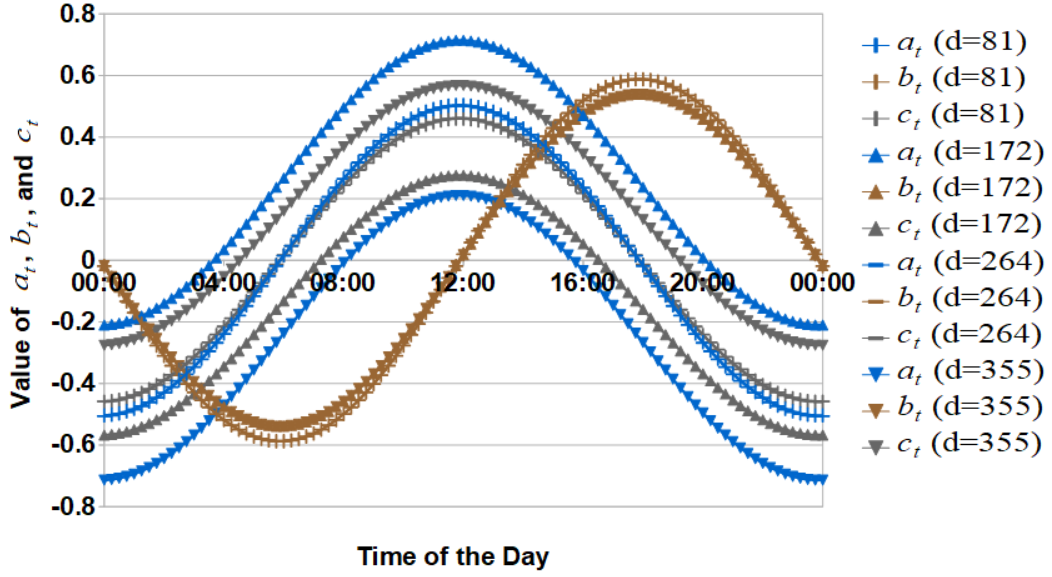
\includegraphics[width=1\columnwidth]{pictures/abc}
\caption[Values of $a_t$, $b_t$, and $c_t$ throughout one day for the spring equinox, summer solstice, autumn equinox, and winter solstice]{Values of $a_t$, $b_t$, and $c_t$ throughout one day for the spring equinox ($d=81$), summer solstice ($d=172$), autumn equinox ($d=264$), and winter solstice ($d=355$). $\gamma$ is set at $36^{\mathrm{o}}$, and the location is Greenwich ($lat=51.4767^{\mathrm{o}}$ North, $lon=0.0003^{\mathrm{o}}$ West) for all scenarios.  \label{abc_values}}
\end{figure}



The following insights are obtained from (\ref{allgemein_AOI3}) to (\ref{allgemein_AOI4}):

\begin{itemize}
\item $a_t$ and $c_t$ are symmetrical to noon. Hence, if $\theta\neq 0^\mathrm{o}$, i.e., $\sin(\theta)\neq 0$, $b_t$ is solely responsible for shifting the energy generation peak towards the morning or afternoon hours. If $\theta$ is orientated eastwards (westwards), then $\theta<0^{\mathrm{o}}$ ($\theta>0^{\mathrm{o}}$), and $\sin(\theta)< 0$ ($\sin(\theta)> 0$), and hence the energy generation peak is shifted toward the morning (afternoon) hours.
\item Also (\ref{I4}) causes an asymmetric energy generation profile if $\theta\neq0^{\mathrm{o}}$. The $\max$ in (\ref{I4}) removes the direct-beam irradiance if the PV cell is illuminated from the back. The more the PV cell is orientated eastwards (westwards), the longer the PV cell is illuminated from the back in the evening (morning) and the more energy is lost in the evening (morning).
\item If the location of the PV cell is on the equator, the PV cell should be installed with the default inclination angle $\gamma=0^\mathrm{o}$ (cf. Table \ref{over}). As a consequence, $\sin(\gamma)=0$, and $b_t=c_t=0$. As a result, any orientation angle can be chosen for a PV cell on the equator because the orientation angle does not affect the energy generation profile of a PV cell on the equator. Figure \ref{fig:June} provides graphically the proof by using the data from PVGIS \cite{PVGIS}.
Hence, orientation angle optimization should be done for PV cells a bit farther away from the equator, where PV cells are not horizontally mounted. Alternatively, PV cells on the equator can be inclined ($\gamma\neq 0^\mathrm{o}$) a bit to facilitate orientation angle optimization at the cost of reducing the average daily energy yield of the PV cells.

\begin{figure}[H]
	\centering
		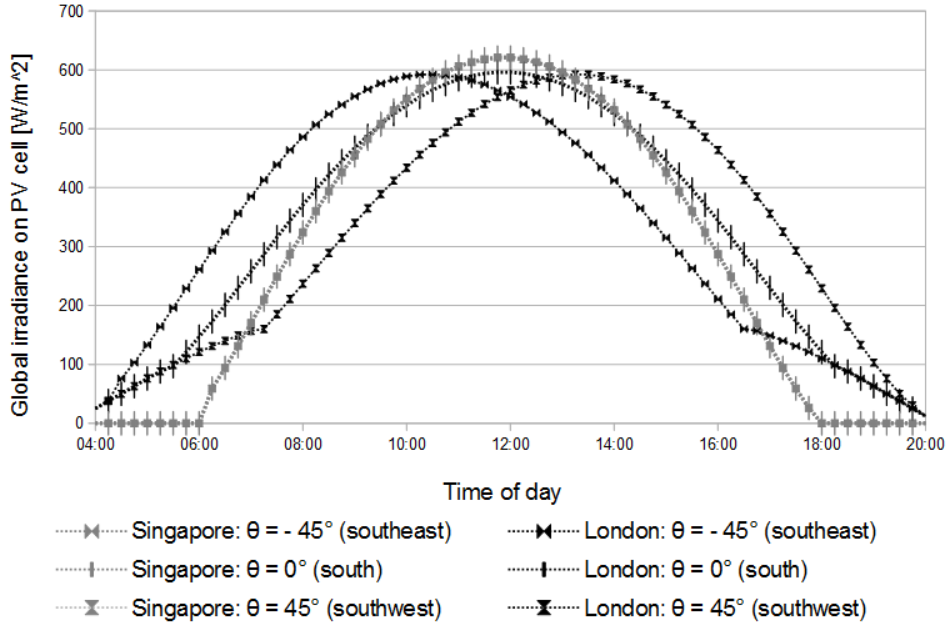
\includegraphics[width=\columnwidth]{pictures/lon-sin}
\caption[Irradiance values of differently oriented PV cells in Greenwich (London, UK) and Singapore]{Irradiance values of differently orientated PV cell installations in Greenwich (temperate zone on northern hemisphere) and Singapore (close to equator) in June. An inclination angle of $38^{\mathrm{o}}$ ($0^{\mathrm{o}}$) was chosen for Greenwich (Singapore).\\ Data source: \cite{PVGIS} \label{fig:June}}

\end{figure}
\item The amplitude of $b_t$ is equal to the amplitude of $c_t$ at the north and south poles, whereas the amplitude of $b_t$ is greater than the amplitude of $c_t$ at any other location. 
\end{itemize}



\section{Results and Discussion\label{results}}
Table \ref{tab:inpu_1} summarizes all parameters and their values. 
The total surface area of the $N$ PV cells, denoted by $A$, the duration of one time step, denoted by $\tau$, and the energy conversion efficiency of the PV cells, denoted by $\eta$, do not appear in (\ref{norma}) anymore due to the normalization of the energy generation in (\ref{norma}). As a result, there is no value assigned to these parameters in Table \ref{tab:inpu_1}.

The derived $I_{\theta}(t)$ values in this thesis were compared with the modeled irradiance values from the PVGIS database (daily data profiles \cite{tool}). Both values were the same. This proves that our derivation and implementation of the irradiance model is correct. The irradiance model implemented in PVGIS \cite{PVGIS} is the Muneer model \cite{muneer}, but it is mentioned on the PVGIS website \cite{method} that the Muneer model performs very similar to the Reindl model. The Reindl model was used in this thesis. 


\begin{longtable}{@{}l*{2}{|l}l@{}}
\caption{\\ Input parameters of system model 1\label{tab:inpu_1}}\\ \toprule
\textbf{Parameter}	&\textbf{Description}				&  \textbf{Value} \\ \midrule
$\alpha$  &Albedo of ground&$0.2$ (Grassland)\\
$\gamma$  &Inclination angle &$36^{\mathrm{o}}$\\
$\delta_d$ &Declination angle & Eq. (\ref{delta})\\
$\zeta_t$  &Zenith angle & Eq. (\ref{zenith})\\
$\eta$  &Energy conversion efficiency of the PV cells & \\
$\theta$  &Orientation angle&$\in [-90^{\mathrm{o}},90^{\mathrm{o}}]$\\
$\theta_1, ..., \theta_N$ &Orientation angles of PV cells $1,..., N$&$\in [-90^{\mathrm{o}},90^{\mathrm{o}}]$\\
$\theta_1^*, ..., \theta_N^*$ &Optimal orientation angles $\theta_1, ..., \theta_N$ &$\in [-90^{\mathrm{o}},90^{\mathrm{o}}]$\\
$\tau$ & Duration of one time step& \\
$\omega_t$ &Hour angle&Figure \ref{hour_angle_graph}\\
$\Delta_1$ &Gain of adding the $1^{\mathrm{st}}$ PV cell&Eq. (\ref{Delta_1})\\
$\Delta_n$ &Gain of adding the $n^{\mathrm{th}}$ PV cell, $n\in\{2, ..., N\}$&Eq. (\ref{Delta_n})\\
$A$ & Total surface area of $N$ PV cells& \\
$A_t$ &Anisotropy index at time step $t$&Eq. (\ref{At}) \\
$AOI_{\theta}(t)$ &Angle of incidence &Eq.  (\ref{allgemein_AOI})\\
$C(t)$ &Energy consumption of BS at time step $t$ &Figures \ref{constant_allgemein} - \ref{residential_allgemein}\\
$C_{\mathrm{bus}}(t)$ & Business-area traffic load profile at time step $t$& Figure \ref{all_consumption_profiles}\\
$C_{\mathrm{con}}(t)$ & Constant traffic load profile at time step $t$&Figure \ref{all_consumption_profiles}\\
$C_{\mathrm{res}}(t)$ &  Residential-area traffic load profile at time step $t$&Figure \ref{all_consumption_profiles}\\
$DHI_t$ &Diffuse horizontal irradiance at time step $t$&PVGIS \cite{PVGIS} \\
$DNI_t$ &Direct normal irradiance at time step $t$  &PVGIS \cite{PVGIS} \\
$E_d$ & Extraterrestrial radiation &Eq. (\ref{extra}) \\
$E_{\mathrm{con}}$ & Solar constant &$1367\frac{\mathrm{W}}{\mathrm{m}^2}$ \cite{Solar_Cell_declination_inclination_angle}\\
$G(t)$ &Energy generation of PV cell/cells at time step $t$& \\
$G^{\text{original}}_{\theta,N}(t)$&Energy generated by one&\\
&PV cell installed with $\theta$ at time step $t$&\\
&($N$ is the total number of PV cells)&Eq. (\ref{normalization})\\
$G_{\theta,N}(t)$ &Normalized energy generated by&\\
& one PV cell installed with $\theta$ at time step $t$&\\
&($N$ is the total number of PV cells)&Eq. (\ref{norma})\\
$G_{(\theta_1, ..., \theta_N)}(t)$ &Normalized total energy&\\
& generated by $N$ PV cells at time step $t$&\\
&installed with $\theta_1, ....,\theta_N$&Eq. (\ref{nor})\\
$GHI_t$ &Global horizontal irradiance at time step $t$  &PVGIS \cite{PVGIS} \\
$I_{\theta}(t)$  &Irradiance on PV cell installed &\\
  & with $\theta$ at time step $t$&Eq. (\ref{I1})\\
$I_{b_\theta}(t)$ &Direct-beam irradiance at time step $t$&Eq.  (\ref{I4})\\
$I_{d_\theta}(t)$ &Sky-diffuse irradiance at time step $t$&Eq.  (\ref{reindl})\\
$I_{g}(t)$ &Ground-reflected irradiance at time step $t$&Eq.   (\ref{I3})\\ 
$N$ &Number of PV cells &$\in \{1,2,3\}$\\
$T$ &Number of time steps&96\\
$a_t$& Independent of $\theta$& Eq. (\ref{a_t})\\
$b_t$& Multiplied by  $\sin(\theta)$ &Eq.  (\ref{b_t})\\
$c_t$& Multiplied by  $\cos(\theta)$&Eq.  (\ref{c_t})\\
$d$ &Day of the year &165 (June)\\
$f(\theta_1, ..., \theta_N)$ &Optimization objective &Eq.  (\ref{optimization_objective})\\
$lat$ &Latitude  &$51.4767^{\mathrm{o}}$ North\\
 &  & (Greenwich)\\
$lon$ &Longitude &$0.0003^{\mathrm{o}}$ West\\
 &&(Greenwich)\\
\bottomrule
\end{longtable}



\subsection{Remarks on the Presentation of the Results\label{results_load_shape}}
The optimal orientation angle(s) will be investigated for 1, 2, and 3 PV cell(s) in Subsections \ref{results_1PV}, \ref{results_2PV}, and \ref{results_3PV}, respectively. The optimal orientation angle will be obtained for each PV cell in the complete range from $- 90^\mathrm{o}$ to $90^\mathrm{o}$ with an angular resolution of $1^\mathrm{o}$.

The graphs in the Table \ref{table_1PV}, Table \ref{table_2PV}, and Table \ref{table_3PV} are generated with MATLAB. The source code of Chapter \ref{Chapter_1} is given in the Appendix B of this thesis and is available on GitHub \cite{DOBEN_GITHUB}.


Normalized energy generation and consumption profiles are used in this thesis. That means the given recommendations in this section can be scaled up for the intended application in the real world. For example, if the derived recommendation for the normalized consumption profile $C(t)$ is to deploy one PV cell with optimal orientation angel $\theta_1^*$,  
that means to deploy several PV cells with the same orientation angle $\theta_1^*$ in the real world if $C(t)$ was the consumption profile of a large-scale BS. Another example, if the derived recommendation for the normalized consumption profile $C(t)$ is to deploy two PV cells with jointly optimized orientation angles $\theta_1^*$ and $\theta_2^*$, that means to deploy several PV cells where half of them are deployed with $\theta_1^*$ and the other half with $\theta_2^*$ in the real world if $C(t)$ was the consumption profile of a large-scale BS. 


\subsubsection{Results for 1 PV Cell (N=1) \label{results_1PV}}

Table \ref{table_1PV} and Table \ref{opt_1PV} show the results for 1 PV cell.

The orientation angle is optimized for three different types of load profiles: the constant load profile $C_{\mathrm{con}}(t)$, the business load profile $C_{\mathrm{bus}}(t)$, and the residential load profile $C_{\mathrm{res}}(t)$ (cf. Figure \ref{all_consumption_profiles}). The left, middle, and right columns in Table \ref{table_1PV} represent the constant, business, and residential load profiles, respectively. Each row in Table \ref{table_1PV} represents the relative relationship between the energy generation profile and energy consumption profile. In other words, the first, second, third, and fourth rows in Table \ref{table_1PV} represent the scenario that the energy generation is significantly smaller, is slightly smaller, is slightly greater, is significantly greater than the energy consumption, denoted by $G<<C$, $G<C$, $G>C$, and $G>>C$, respectively. The red lines in Table \ref{table_1PV} are the optimal orientation angles.

\newpage

\newcounter{tablemajor}
\renewcommand\thetable{\arabic{tablemajor}.\arabic{table}}
\newcommand*\settablecounter[2]{%
        \setcounter{tablemajor}{#1}%
        \setcounter{table}{#2-1}%
}
\settablecounter{2}{3}

\begin{sidewaystable}
 \centering
\captionsetup{justification=centering}
\caption{\\ Summary of all optimal orientation angles for 1 PV cell with the different load profiles from Table \ref{table_1PV} \label{opt_1PV}}
  \begin{tabular}
      {c|c||c|c|c} 
		\multicolumn{2}{c||}{ }	&  Constant Load Profile  & Business Load Profile  &  Residential Load Profile  \\
			
      \hline\hline
						  &&  Table cell (a) of Table \ref{table_1PV}:    &Table cell (b) of Table \ref{table_1PV}:     &Table cell (c) of Table \ref{table_1PV}:     \\  
			  &&  1 optimal line   & 1 optimal line &1 optimal line  \\  
				
				 $G<<C$&      $\theta_1^*$     &     $\in \{0^\mathrm{o}\}$     &     $\in \{0^\mathrm{o}\}$   &  $\in \{0^\mathrm{o}\}$\\\cline{2-5}		
				
				&   $f(0^\mathrm{o})$ & 60.0712& 101.3440 & 100.2310 \\\cline{2-5}	
				
				& $f(\theta_1^*)$  & 60.0712& 101.3440 &	100.2310\\\cline{2-5}	
				
				&  $\Delta_1$  & 0&  0 &	0\\ \hline
	
				&&  Table cell (d) of Table \ref{table_1PV}:    &Table cell (e) of Table \ref{table_1PV}:     &Table cell (f) of Table \ref{table_1PV}:     \\  
				& &2 optimal lines    & 1 optimal line    &1 optimal line   \\  
				
			$G<C$	&      $\theta_1^*$     &    $\in \{-12^\mathrm{o},12^\mathrm{o}\}$  &  $\in \{32^\mathrm{o}\}$      &  $\in \{7^\mathrm{o}\}$  \\\cline{2-5}	
				
				 &   $f(0^\mathrm{o})$ &43.7613 &  35.2500 &81.3698 \\\cline{2-5}	
					
				&    $f(\theta_1^*)$& 43.7530& 34.3548 & 81.3530 \\\cline{2-5}	
				
				&  $\Delta_1$  & 0.0083&   0.8952&	0.0168\\ \hline					
				
				&&  Table cell (g) of Table \ref{table_1PV}:    &Table cell (h) of Table \ref{table_1PV}:     &Table cell (i) of Table \ref{table_1PV}:     \\  
				&  & 2 optimal lines     & 1 optimal line    &1 optimal line  \\  
				
				$G>>C$	 &      $\theta_1^*$     &     $\in \{-35^\mathrm{o},35^\mathrm{o}\}$  &    $\in \{59^\mathrm{o}\}$    &$\in \{-70^\mathrm{o}\}$       \\\cline{2-5}
						
			&   $f(0^\mathrm{o})$ &29.9956 & 12.3939 &59.0301 \\\cline{2-5}	
				
				&   $f(\theta_1^*)$   & 29.9630&  10.0621 &	57.7670 \\\cline{2-5}	
				
				&  $\Delta_1$  &0.0326 & 2.3318&	1.2631\\ \hline		
					
					&&  Table cell (j) of Table \ref{table_1PV}:    &Table cell (k) of Table \ref{table_1PV}:     &Table cell (l) of Table \ref{table_1PV}:     \\  
				 & &  2 optimal lines    & 1 optimal line    &1 optimal line   \\  
				
					$G>C$	 &      $\theta_1^*$     &  $\in \{-90^\mathrm{o},90^\mathrm{o}\}$&    $\in \{90^\mathrm{o}\}$  &   $\in \{-90^\mathrm{o}\}$  \\\cline{2-5}	
					
		&   $f(0^\mathrm{o})$ &12.6629 &  3.3316&27.6658 \\\cline{2-5}	
				
					&   $f(\theta_1^*)$ & 12.2800&  1.2400 &	26.1165 \\\cline{2-5}	
				
				&  $\Delta_1$  & 0.3829&  2.0916 &	1.5493
  \end{tabular}
\end{sidewaystable}


\settablecounter{2}{2}
\begin{table}[H] 
 \centering
\leftskip=-2cm
\captionsetup{justification=centering}
\caption{\\ Orientation angles optimization for 1 PV cell with different load profiles \label{table_1PV}}
  \begin{tabular}
      {@{ }m{0.11\columnwidth}@{ }||@{ }M{0.35\columnwidth}@{ }|@{ }M{0.35\columnwidth}@{ }|@{ }M{0.35\columnwidth}@{ }} 
			&  Constant Load Profile &  Business Load Profile & Residential Load Profile \\
			
			\hline\hline 
			   &  Table cell (a): & Table cell (b): &  Table cell (c): \\
			
      $G<<C$ &  \vspace{0.1cm}  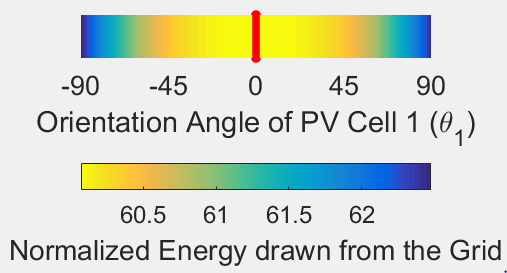
\includegraphics[scale=0.45]{pictures/results/rein_1PV_scale1_offset1_con}  & \vspace{0.1cm} 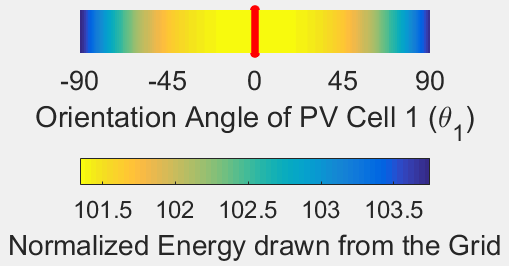
\includegraphics[scale=0.45]{pictures/results/rein_1PV_scale1_offset1_bis}  & \vspace{0.1cm} 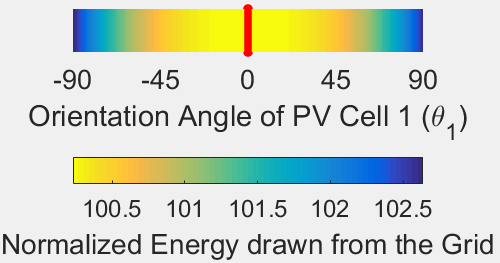
\includegraphics[scale=0.45]{pictures/results/rein_1PV_scale1_offset1_res} \\
			
			 	
							  &  $\quad C(t)= 1$  &   $\quad C(t)=C_{\mathrm{bus}}(t) + 1$ &  $\quad C(t)=C_{\mathrm{res}}(t) + 1$ \\ 	
									
									&  (Figure \ref{constant_allgemein} yellow line)  &   (Figure \ref{business_allgemein} yellow line)&  (Figure \ref{residential_allgemein} yellow line) \\  \hline 		
				   &  Table cell (d): & Table cell (e): &  Table cell (f): \\
						   $G<C$ & \vspace{0.1cm}  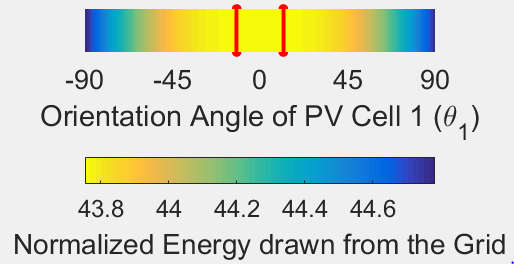
\includegraphics[scale=0.45]{pictures/results/rein_1PV_scale1_offset0_8_con}  & \vspace{0.1cm} 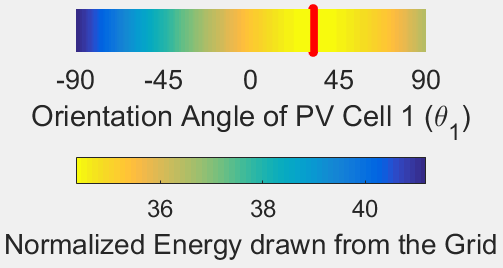
\includegraphics[scale=0.45]{pictures/results/rein_1PV_scale1_offset0_3_bis}  &
      \vspace{0.1cm} 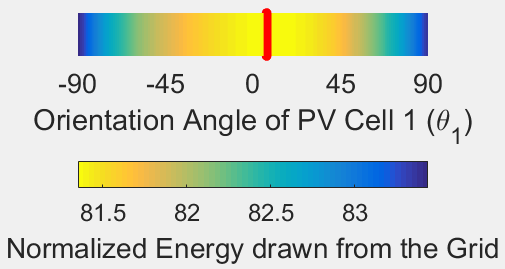
\includegraphics[scale=0.45]{pictures/results/rein_1PV_scale1_offset0_8_res} \\
		
				
					  &   $\quad C(t)= 0.8$  &   $\quad C(t)=C_{\mathrm{bus}}(t) + 0.3$ & $\quad C(t)=C_{\mathrm{res}}(t) + 0.8$\\
						
						  &  (Figure \ref{constant_allgemein} gray line)& (Figure \ref{business_allgemein} green line)&  (Figure \ref{residential_allgemein} green line)\\ \hline
				
				 &  Table cell (g): & Table cell (h): &  Table cell (i): \\
				
				   $G>C$ & \vspace{0.1cm} 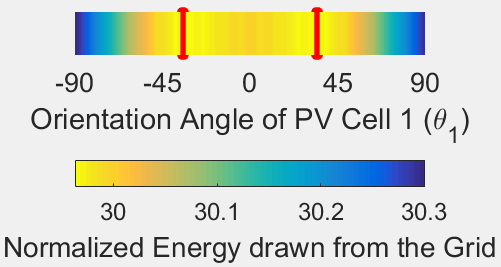
\includegraphics[scale=0.45]{pictures/results/rein_1PV_scale1_offset0_6_con}  & \vspace{0.1cm} 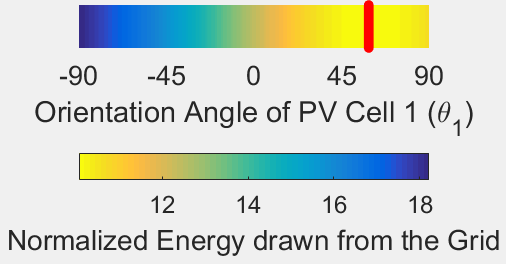
\includegraphics[scale=0.45]{pictures/results/rein_1PV_scale1_offset0_bis}         & \vspace{0.1cm} 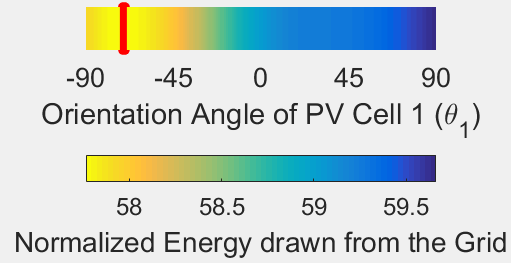
\includegraphics[scale=0.45]{pictures/results/rein_1PV_scale1_offset0_5_res} \\
			
				 &  $\quad C(t)= 0.6$ &   $\quad C(t)=C_{\mathrm{bus}}(t)$ &  $\quad C(t)=C_{\mathrm{res}}(t) + 0.5$ \\  	
				
					 &  (Figure \ref{constant_allgemein} light blue line)&  (Figure \ref{business_allgemein} gray line)&  (Figure \ref{residential_allgemein} gray line)\\  \hline 	
					
						 &  Table cell (j): & Table cell (k): &  Table cell (l): \\
      $G>>C$ &  \vspace{0.1cm} 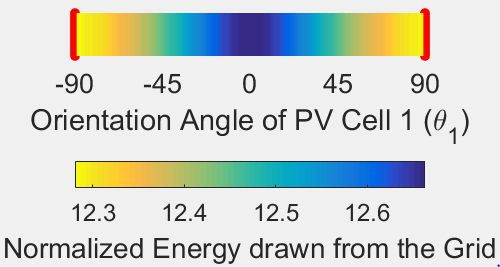
\includegraphics[scale=0.45]{pictures/results/rein_1PV_scale1_offset0_3_con}  & \vspace{0.1cm} 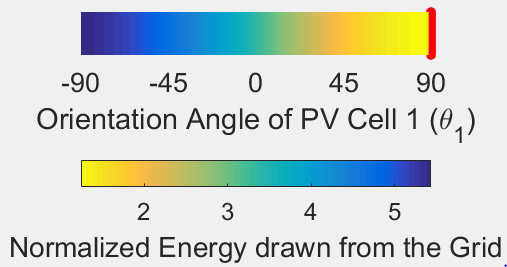
\includegraphics[scale=0.45]{pictures/results/rein_1PV_scale0_5_offset0_bis}  &
      \vspace{0.1cm} 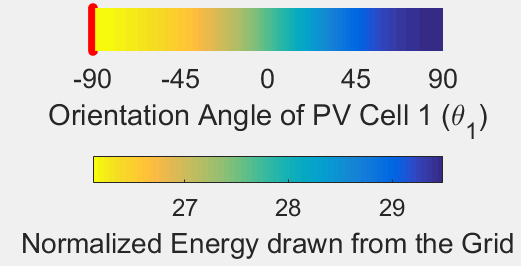
\includegraphics[scale=0.45]{pictures/results/rein_1PV_scale1_offset0_res} \\
			

			&   $\quad C(t)= 0.3$ &   $\quad C(t)=\frac{1}{2}C_{\mathrm{bus}}(t)$ &  $\quad C(t)=C_{\mathrm{res}}(t)$  \\
	
			
			&\vspace{-0.5cm}  (Figure \ref{constant_allgemein} black line)& \vspace{-0.5cm}   (Figure \ref{business_allgemein} light blue line)&\vspace{0.3cm}   (Figure \ref{residential_allgemein} light blue line) 
			
		
  \end{tabular}
\end{table}




\newpage




\subsubsection{Results for 2 PV Cells (N=2) \label{results_2PV}}

Table \ref{table_2PV} and Table \ref{opt_2PV} show the results for 2 PV cells.

The orientation angles are optimized for three different types of load profiles: the constant load profile $C_{\mathrm{con}}(t)$, the business load profile $C_{\mathrm{bus}}(t)$, and the residential load profile $C_{\mathrm{res}}(t)$ (cf. Figure \ref{all_consumption_profiles}). The left, middle, and right columns in Table \ref{table_2PV} represent the constant, business, and residential load profiles, respectively. Each row in Table \ref{table_2PV} represents the relative relationship between the energy generation profile and energy consumption profile. In other words, the first, second, third, and fourth rows in Table \ref{table_2PV} represent the scenario that the energy generation is significantly smaller, is slightly smaller, is slightly greater, is significantly greater than the energy consumption, denoted by $G<<C$, $G<C$, $G>C$, and $G>>C$, respectively. The red points in Table \ref{table_2PV} are the optimal orientation angles.
Each square in Table \ref{table_2PV} has one line of symmetry \mbox{$L$:= \{$(\theta_1,\theta_2)\in [-90^\mathrm{o},90^\mathrm{o}]^2 \enskip|\theta_1=\theta_2$\}}.




\newpage
\settablecounter{2}{5}

\begin{sidewaystable}
 \centering
\captionsetup{justification=centering}
\caption{\\ Summary of all optimal orientation angles for 2 PV cells with the different load profiles from Table \ref{table_2PV} \label{opt_2PV}}
  \begin{tabular}
      {c|c||c|c|c} 
			\multicolumn{2}{c||}{}   &Constant Load Profile  &  Business Load Profile  &  Residential Load Profile  \\
			
      \hline\hline
			
			&&  Table cell (a) of Table \ref{table_2PV}:    &Table cell (b) of Table \ref{table_2PV}:     &Table cell (c) of Table \ref{table_2PV}:     \\  
			  & & 1 optimal point   & 1 optimal point  &1 optimal point   \\  
				
				$G<<C$ &  \  $(\theta_1^*,\theta_2^*)$ \  & $\in \{(0^\mathrm{o},0^\mathrm{o})\}$    & $\in \{(0^\mathrm{o},0^\mathrm{o})\}$ &$\in \{(0^\mathrm{o},0^\mathrm{o})\}$ \\\cline{2-5}		
				
					&   $f(\theta_1^*,\theta_2^*)$ &60.0712  &101.3440 &	100.2310\\\cline{2-5}	
					
					&  $\Delta_2$  &0  & 0 &0\\ \hline
					
					&&  Table cell (d) of Table \ref{table_2PV}:    &Table cell (e) of Table \ref{table_2PV}:     &Table cell (f) of Table \ref{table_2PV}:     \\  
				 & & 2 optimal points     & 1 optimal point   &2 optimal points    \\  
				
			$G<C$ &  \  $(\theta_1^*,\theta_2^*)$ \  &  $\in \{(-48^\mathrm{o},48^\mathrm{o}),(48^\mathrm{o},-48^\mathrm{o})\}$     & $\in \{(32^\mathrm{o},32^\mathrm{o})\}$  &$\in \{(-26^\mathrm{o},35^\mathrm{o}),(35^\mathrm{o},-26^\mathrm{o})\}$  \\\cline{2-5}	
	
	&    $f(\theta_1^*,\theta_2^*)$& 51.0780&  34.3548 & 81.2773\\\cline{2-5}	
		
		&  $\Delta_2$  &0.3918 &  0&	0.0757\\ \hline
				
				
				&&  Table cell (g) of Table \ref{table_2PV}:    &Table cell (h) of Table \ref{table_2PV}:     &Table cell (i) of Table \ref{table_2PV}:     \\  
				 &  &2 optimal points    & 1 optimal point    &2 optimal points    \\  
				
					$G>C$ &  \  $(\theta_1^*,\theta_2^*)$ \  & $\in \{(-69^\mathrm{o},69^\mathrm{o}),(69^\mathrm{o},-69^\mathrm{o})\}$   & $\in \{(59^\mathrm{o},59^\mathrm{o})\}$ & $\in \{(-90^\mathrm{o},90^\mathrm{o}),(90^\mathrm{o},-90^\mathrm{o})\}$ \\\cline{2-5}	
					
							&  $f(\theta_1^*,\theta_2^*)$  &42.7376&   10.0621 &	 57.2246\\\cline{2-5}	
							
							&  $\Delta_2$  &1.0154 &  0&	0.5424\\ \hline
							
							&&  Table cell (j) of Table \ref{table_2PV}:    &Table cell (k) of Table \ref{table_2PV}:     &Table cell (l) of Table \ref{table_2PV}:     \\  
				 & & 2 optimal points    & 1 optimal point    &1 optimal point \\  
				
				$G>>C$ &  \  $(\theta_1^*,\theta_2^*)$ \  & $\in \{(-90^\mathrm{o},90^\mathrm{o}),(90^\mathrm{o},-90^\mathrm{o})\}$  & $\in \{(90^\mathrm{o},90^\mathrm{o})\}$   & 	$\in \{(-90^\mathrm{o},-90^\mathrm{o})\}$\\\cline{2-5}	
				
				&    $f(\theta_1^*,\theta_2^*)$ & 27.8739&  1.2400&26.1165\\\cline{2-5}	
				
				&  $\Delta_2$  & 2.0891&  0&	0\\ 
  \end{tabular}
\end{sidewaystable}


\settablecounter{2}{4}
\begin{table}[H] 
 \centering
\vspace{-0.5cm}\leftskip=-1.5cm
\captionsetup{justification=centering}
\caption{\\ Orientation angles optimization for 2 PV cells with different load profiles \label{table_2PV}}
  \begin{tabular}
      {@{ }m{0.11\columnwidth}@{ }||@{ }M{0.34\columnwidth}@{ }|@{ }M{0.34\columnwidth}@{ }|@{ }M{0.34\columnwidth}@{ }} 
			&  Constant Load Profile &  Business Load Profile & Residential Load Profile \\ \hline\hline
			&  Table cell (a): & Table cell (b): &  Table cell (c): \\
			  $G<<C$ & \vspace{0.1cm}  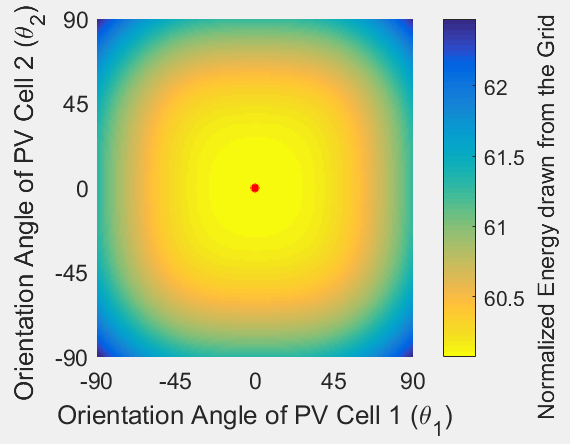
\includegraphics[width=0.34\columnwidth, height=4.5cm]{pictures/results/rein_2PV_scale1_offset1_con}  & \vspace{0.1cm} 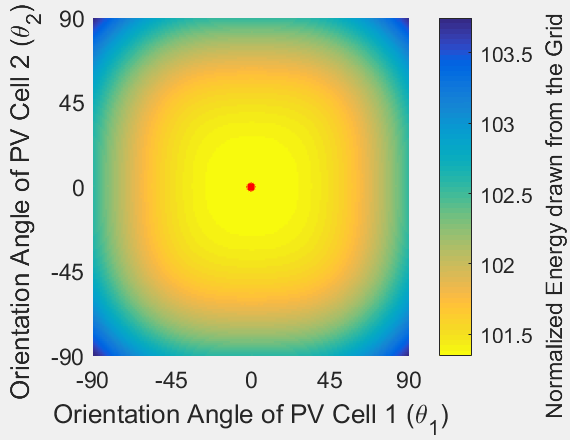
\includegraphics[width=0.34\columnwidth, height=4.5cm]{pictures/results/rein_2PV_scale1_offset1_bis}  &
      \vspace{0.1cm} 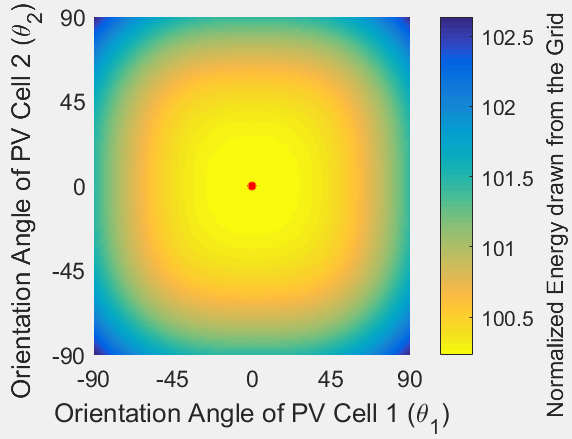
\includegraphics[width=0.34\columnwidth, height=4.5cm]{pictures/results/rein_2PV_scale1_offset1_res} \\
		
			
			
			  &  $\quad C(t)= 1$  &   $\quad C(t)=C_{\mathrm{bus}}(t) + 1$  &  $\quad C(t)=C_{\mathrm{res}}(t) + 1$ \\  		
				
				&  (Figure \ref{constant_allgemein} yellow line)  &  (Figure \ref{business_allgemein} yellow line)&  (Figure \ref{residential_allgemein} yellow line)\\  \hline 		
				&  Table cell (d): & Table cell (e): &  Table cell (f): \\
						   $G<C$ & \vspace{0.1cm}  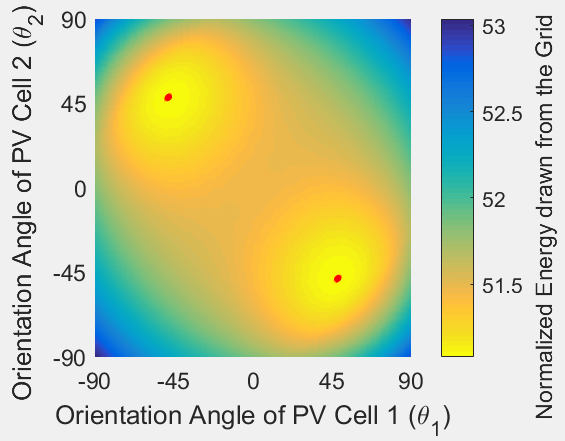
\includegraphics[width=0.34\columnwidth, height=4.5cm]{pictures/results/rein_2PV_scale1_offset0_9_con}  & \vspace{0.1cm} 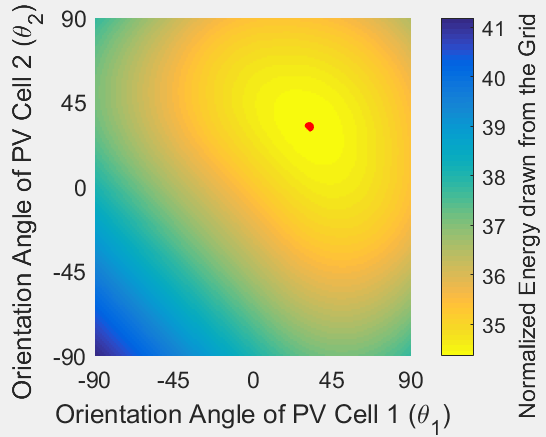
\includegraphics[width=0.34\columnwidth, height=4.5cm]{pictures/results/rein_2PV_scale1_offset0_3_bis}  &
      \vspace{0.1cm} 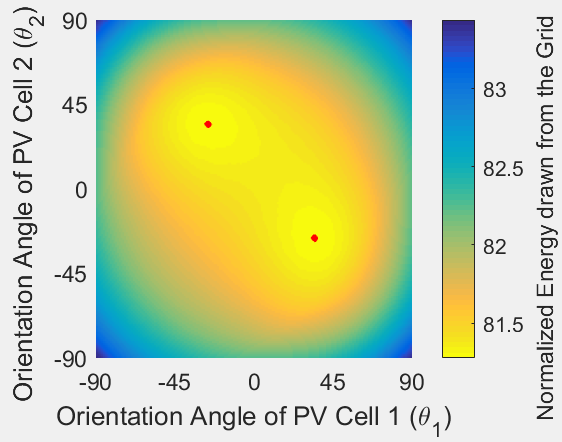
\includegraphics[width=0.34\columnwidth, height=4.5cm]{pictures/results/rein_2PV_scale1_offset0_8_res} \\
			
			  &   $\quad C(t)= 0.9$ &   $\quad C(t)=C_{\mathrm{bus}}(t) + 0.3$ &  $\quad C(t)=C_{\mathrm{res}}(t) + 0.8$ \\  
				
				 &   (Figure \ref{constant_allgemein} green line)&  (Figure \ref{business_allgemein} green line)& (Figure \ref{residential_allgemein} green line)\\ \hline 
				
				&  Table cell (g): & Table cell (h): &  Table cell (i): \\
				  $G>C$ & \vspace{0.1cm} 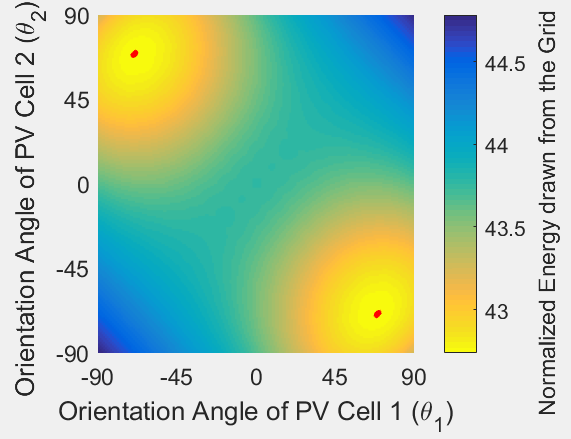
\includegraphics[width=0.34\columnwidth, height=4.5cm]{pictures/results/rein_2PV_scale1_offset0_8_con}  & \vspace{0.1cm} 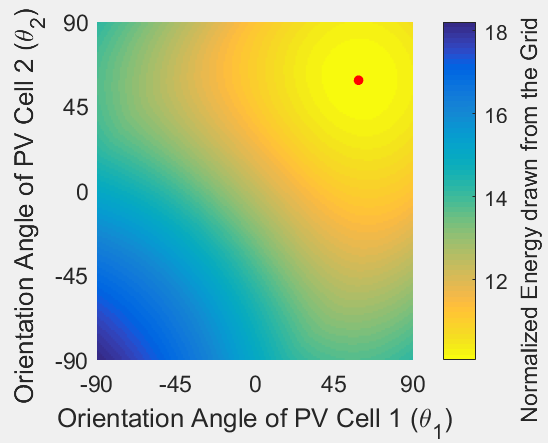
\includegraphics[width=0.34\columnwidth, height=4.5cm]{pictures/results/rein_2PV_scale1_offset0_bis}         & \vspace{0.1cm} 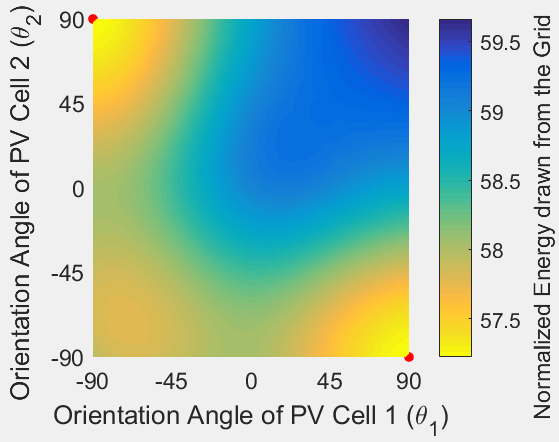
\includegraphics[width=0.34\columnwidth, height=4.5cm]{pictures/results/rein_2PV_scale1_offset0_5_res} \\
			
			  &   $\quad C(t)= 0.8$ &   $\quad C(t)=C_{\mathrm{bus}}(t)$  &  $\quad C(t)=C_{\mathrm{res}}(t) + 0.5$ \\  
					
					&   (Figure \ref{constant_allgemein} gray line)&  (Figure \ref{business_allgemein} gray line)&  (Figure \ref{residential_allgemein} gray line)\\  \hline 	
						
						&  Table cell (j): & Table cell (k): &  Table cell (l): \\
      $G>>C$ &  \vspace{0.1cm} 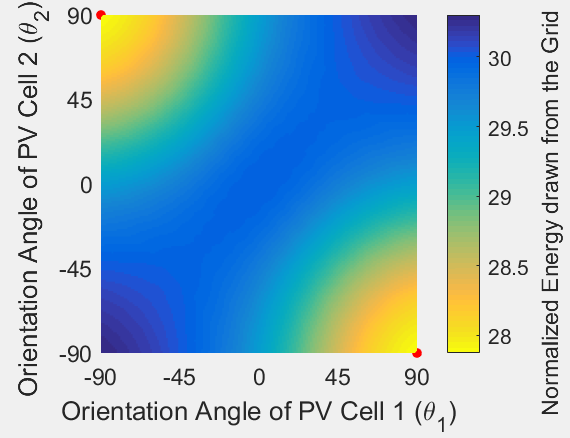
\includegraphics[width=0.34\columnwidth, height=4.5cm]{pictures/results/rein_2PV_scale1_offset0_6_con}  & \vspace{0.1cm} 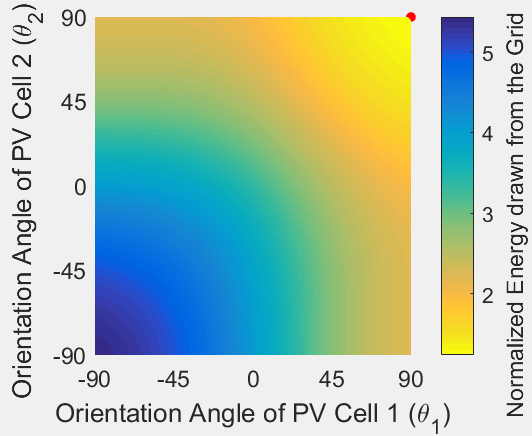
\includegraphics[width=0.34\columnwidth, height=4.5cm]{pictures/results/rein_2PV_scale0_5_offset0_bis}  &
      \vspace{0.1cm} 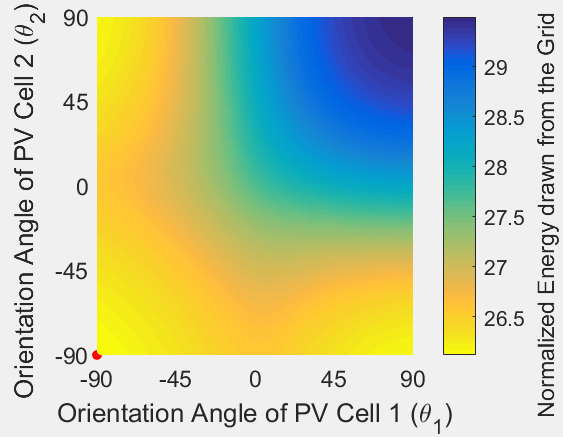
\includegraphics[width=0.34\columnwidth, height=4.5cm]{pictures/results/rein_2PV_scale1_offset0_res} \\
			
			  &   $\quad C(t)= 0.6$ &   $\quad C(t)=\frac{1}{2}C_{\mathrm{bus}}(t)$  & $\quad C(t)=C_{\mathrm{res}}(t) $ \\
				
							  & \vspace{-0.2cm}  (Figure \ref{constant_allgemein} light blue line)&  \vspace{-0.2cm}  (Figure \ref{business_allgemein} light blue line)&\vspace{0.3cm}   (Figure \ref{residential_allgemein} light blue line) 
			
		
  \end{tabular}
\end{table}


\newpage


\subsubsection{Results for 3 PV Cells (N=3) \label{results_3PV}}

Table \ref{table_3PV} and Table \ref{opt_3PV} show the results for 3 PV cells.

The orientation angles are optimized for three different types of load profiles: the constant load profile $C_{\mathrm{con}}(t)$, the business load profile $C_{\mathrm{bus}}(t)$, and the residential load profile $C_{\mathrm{res}}(t)$ (cf. Figure \ref{all_consumption_profiles}). The left, middle, and right columns in Table \ref{table_3PV} represent the constant, business, and residential load profiles, respectively. Each row in Table \ref{table_3PV} represents the relative relationship between the energy generation profile and energy consumption profile. In other words, the first, second, third, and fourth rows in Table \ref{table_3PV} represent the scenario that the energy generation is significantly smaller, is slightly smaller, is slightly greater, is significantly greater than the energy consumption, denoted by $G<<C$, $G<C$, $G>C$, and $G>>C$, respectively. The red points in each cube in Table \ref{table_3PV} are the optimal orientation angles.
Each cube in Table \ref{table_3PV} has three planes of symmetry as follows:


\begin{align}
&P_1:= \{(\theta_1,\theta_2,\theta_3)\in [-90^\mathrm{o},90^\mathrm{o}]^3 \enskip|\theta_2=\theta_3\},\\ 
&P_2:= \{(\theta_1,\theta_2,\theta_3)\in [-90^\mathrm{o},90^\mathrm{o}]^3 \enskip |\theta_1=\theta_3\}, \text{ and}\\ 
&P_3:= \{(\theta_1,\theta_2,\theta_3)\in [-90^\mathrm{o},90^\mathrm{o}]^3 \enskip |\theta_1=\theta_2\}.
\end{align}

The y-axis ($\theta_2$-axis) is reversed in all business load profile scenarios (second column of Table \ref{table_3PV}) so that the optimal points (red points) are visible. Because it is not possible to show all values from a solid 3D cube on a 2D paper, every solid cube in Table \ref{table_3PV} is visualized by 6 planes slicing through the cube. The six planes are

\begin{align}
&S_1:= \{(\theta_1,\theta_2,\theta_3)\in [-90^\mathrm{o},90^\mathrm{o}]^3 \enskip|\theta_3=90^\mathrm{o}\}, \\
&S_2:= \{(\theta_1,\theta_2,\theta_3)\in [-90^\mathrm{o},90^\mathrm{o}]^3 \enskip|\theta_3=45^\mathrm{o}\}, \\
&S_3:= \{(\theta_1,\theta_2,\theta_3)\in [-90^\mathrm{o},90^\mathrm{o}]^3 \enskip|\theta_3=0^\mathrm{o}\}, \\
&S_4:= \{(\theta_1,\theta_2,\theta_3)\in [-90^\mathrm{o},90^\mathrm{o}]^3 \enskip|\theta_3=-45^\mathrm{o}\},\\ 
&S_5:= \{(\theta_1,\theta_2,\theta_3)\in [-90^\mathrm{o},90^\mathrm{o}]^3 \enskip|\theta_3=-90^\mathrm{o}\}, \text{ and}\\ 
&S_6:= \{(\theta_1,\theta_2,\theta_3)\in [-90^\mathrm{o},90^\mathrm{o}]^3 \enskip|\theta_2=0^\mathrm{o}\}.
\end{align}

The optimal orientation angles (red points in Table \ref{table_3PV}) might float between the six slicing planes. Table \ref{opt_3PV} presents the exact values of the optimal orientation angles, hence the exact position of the red points in the cube. 



\newpage



\settablecounter{2}{7}
\begin{sidewaystable}
\centering
\captionsetup{justification=centering}
\caption{\\ Summary of all optimal orientation angles for 3 PV cells with the different load profiles from Table \ref{table_3PV} \label{opt_3PV}}
  \begin{tabular}
      {c|c||c|c|c} 
			\multicolumn{2}{c||}{ }& Constant Load Profile & Business Load Profile   &  Residential Load Profile  \\
			
      \hline\hline
			
			&&  Table cell (a) of Table \ref{table_3PV}:    &Table cell (b) of Table \ref{table_3PV}:     &Table cell (c) of Table \ref{table_3PV}:     \\  
			  &  &  1 optimal point     & 1 optimal point   &1 optimal point    \\  
				
				$G<<C$ &     $(\theta_1^*,\theta_2^*,\theta_3^*)$      &   $\in \{(0^\mathrm{o},0^\mathrm{o},0^\mathrm{o})\}$      &     $\in \{(0^\mathrm{o},0^\mathrm{o},0^\mathrm{o})\}$&         $\in \{(0^\mathrm{o},0^\mathrm{o},0^\mathrm{o})\}$   \\\cline{2-5}		
				
				&  $f(\theta_1^*,\theta_2^*,\theta_3^*)$  &60.0712& 101.3440&	 100.2310\\\cline{2-5}	
				
				&  $\Delta_3$  &0  &0 &	0\\ \hline
				
				
							&&  Table cell (d) of Table \ref{table_3PV}:    &Table cell (e) of Table \ref{table_3PV}:     &Table cell (f) of Table \ref{table_3PV}:     \\  
	  &&  6 optimal points    &1 optimal point    &3 optimal points   \\ 
				
		
				
		 &	$(\theta_1^*,\theta_2^*,\theta_3^*)$ 	&    $\in \{(-55^\mathrm{o},42^\mathrm{o},42^\mathrm{o})$, $(-42^\mathrm{o},-42^\mathrm{o},55^\mathrm{o})$,   & & 	$\in \{(-33^\mathrm{o},31^\mathrm{o},31^\mathrm{o})$,  \\ 
			 	
	$G<C$ 		 &&     $(-42^\mathrm{o},55^\mathrm{o},-42^\mathrm{o})$, $(42^\mathrm{o},-55^\mathrm{o},42^\mathrm{o})$, &$\in \{(32^\mathrm{o},32^\mathrm{o},32^\mathrm{o})\}$&  $(31^\mathrm{o},-33^\mathrm{o},31^\mathrm{o})$,  \\ 
				
			 &	& $(42^\mathrm{o},42^\mathrm{o},-55^\mathrm{o})$, $(55^\mathrm{o},-42^\mathrm{o},-42^\mathrm{o})\}$& &   $(31^\mathrm{o},31^\mathrm{o},-33^\mathrm{o})\}$ \\\cline{2-5}	
			
			&    $f(\theta_1^*,\theta_2^*,\theta_3^*)$        &     51.1204     &34.3548&   81.2783  \\\cline{2-5}	
				
							&  $\Delta_3$  &-0.0424 &  0 &	-0.001\\ \hline	
				
				
							&&  Table cell (g) of Table \ref{table_3PV}:    &Table cell (h) of Table \ref{table_3PV}:     &Table cell (i) of Table \ref{table_3PV}:     \\  
				&    &  6 optimal points    &1 optimal point    &3 optimal points  \\ 
				
				
				&$(\theta_1^*,\theta_2^*,\theta_3^*)$  & $\in \{(-76^\mathrm{o},60^\mathrm{o},60^\mathrm{o})$, $(-60^\mathrm{o},-60^\mathrm{o},76^\mathrm{o})$,  & &	$\in \{(-85^\mathrm{o},-85^\mathrm{o},87^\mathrm{o})$, \\ 
				
				$G>C$ 	& &  $(-60^\mathrm{o},76^\mathrm{o},-60^\mathrm{o})$, $(60^\mathrm{o},-76^\mathrm{o},60^\mathrm{o})$,&  $\in \{(59^\mathrm{o},59^\mathrm{o},59^\mathrm{o})\}$ &	$(-85^\mathrm{o},87^\mathrm{o},-85^\mathrm{o})$, \\ 
				
					& & $(60^\mathrm{o},60^\mathrm{o},-76^\mathrm{o})$, $(76^\mathrm{o},-60^\mathrm{o},-60^\mathrm{o})\}$  & &	 $(87^\mathrm{o},-85^\mathrm{o},-85^\mathrm{o})\}$ \\\cline{2-5}	
					
								&       $f(\theta_1^*,\theta_2^*,\theta_3^*)$    &      42.8827   & 10.0621      &   57.2542    \\\cline{2-5}		
					
					&  $\Delta_3$  &-0.1451 &  0&	-0.0296\\ \hline		
				
				
							&&  Table cell (j) of Table \ref{table_3PV}:    &Table cell (k) of Table \ref{table_3PV}:     &Table cell (l) of Table \ref{table_3PV}:     \\  
				&  & 6 optimal points    & 1 optimal point   &3 optimal points    \\ 
				
				
				& $(\theta_1^*,\theta_2^*,\theta_3^*)$ &    $\in \{(-90^\mathrm{o},-90^\mathrm{o},90^\mathrm{o})$, $(-90^\mathrm{o},90^\mathrm{o},-90^\mathrm{o})$, & &	$\in \{(-90^\mathrm{o},-90^\mathrm{o},90^\mathrm{o})$,\\
					$G>>C$ 	&&    $(-90^\mathrm{o},90^\mathrm{o},90^\mathrm{o})$, $(90^\mathrm{o},-90^\mathrm{o},-90^\mathrm{o})$,  &  $\in \{(90^\mathrm{o},90^\mathrm{o},90^\mathrm{o})\}$&	 $(-90^\mathrm{o},90^\mathrm{o},-90^\mathrm{o})$,\\			

				&&    $(90^\mathrm{o},-90^\mathrm{o},90^\mathrm{o})$, $(90^\mathrm{o},90^\mathrm{o},-90^\mathrm{o})\}$ & &	 $(90^\mathrm{o},-90^\mathrm{o},-90^\mathrm{o})\}$\\\cline{2-5}
					
							&      $f(\theta_1^*,\theta_2^*,\theta_3^*)$    &     28.2100   &     1.2400   &   25.9671    \\\cline{2-5}		
				
				&  $\Delta_3$  & -0.3361& 0 &	0.1494
  \end{tabular}
\end{sidewaystable}




\settablecounter{2}{6}
\begin{table}[H] 
 \centering
\vspace{-0.5cm}\leftskip=-1.5cm
\captionsetup{justification=centering}
\caption{\\ Orientation angles optimization for 3 PV cells with different load profiles \label{table_3PV} }
  \begin{tabular}
      {@{ }m{0.11\columnwidth}@{ }||@{ }M{0.34\columnwidth}@{ }|@{ }M{0.34\columnwidth}@{ }|@{ }M{0.34\columnwidth}@{ }} 
			&  Constant Load Profile &  Business Load Profile & Residential Load Profile \\
			
      \hline\hline 
			
			&  Table cell (a): & Table cell (b): &  Table cell (c): \\
			$G<<C$ &  \vspace{0.1cm}  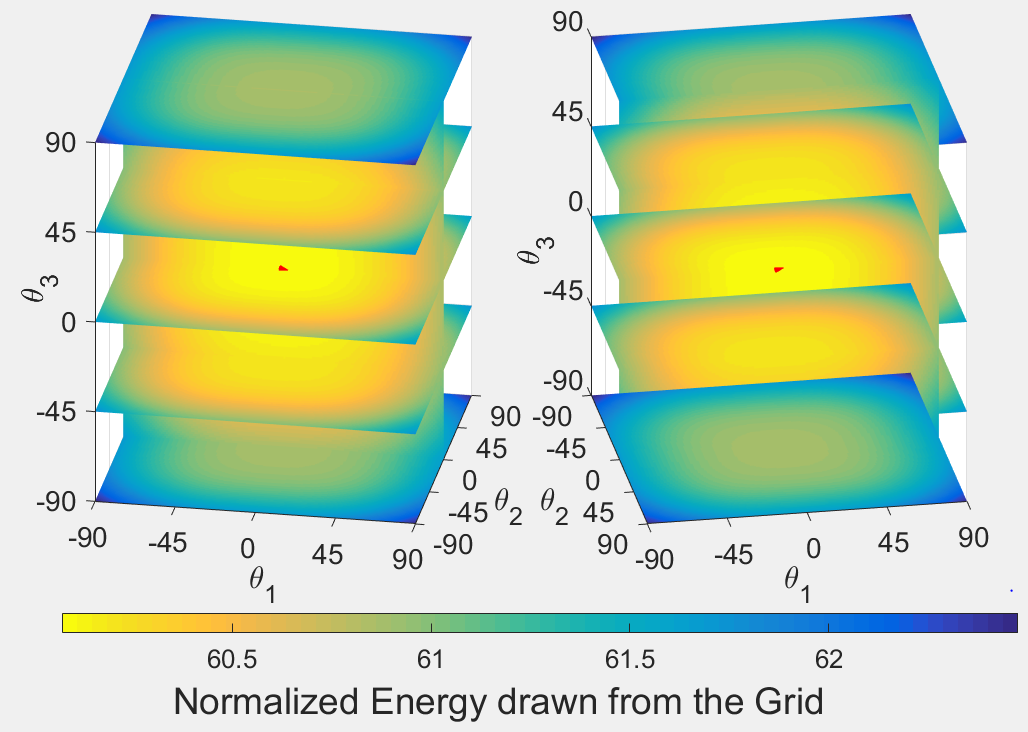
\includegraphics[width=0.34\columnwidth, height=4.6cm]{pictures/results/rein_3PV_scale1_offset1_con}  & \vspace{0.1cm} 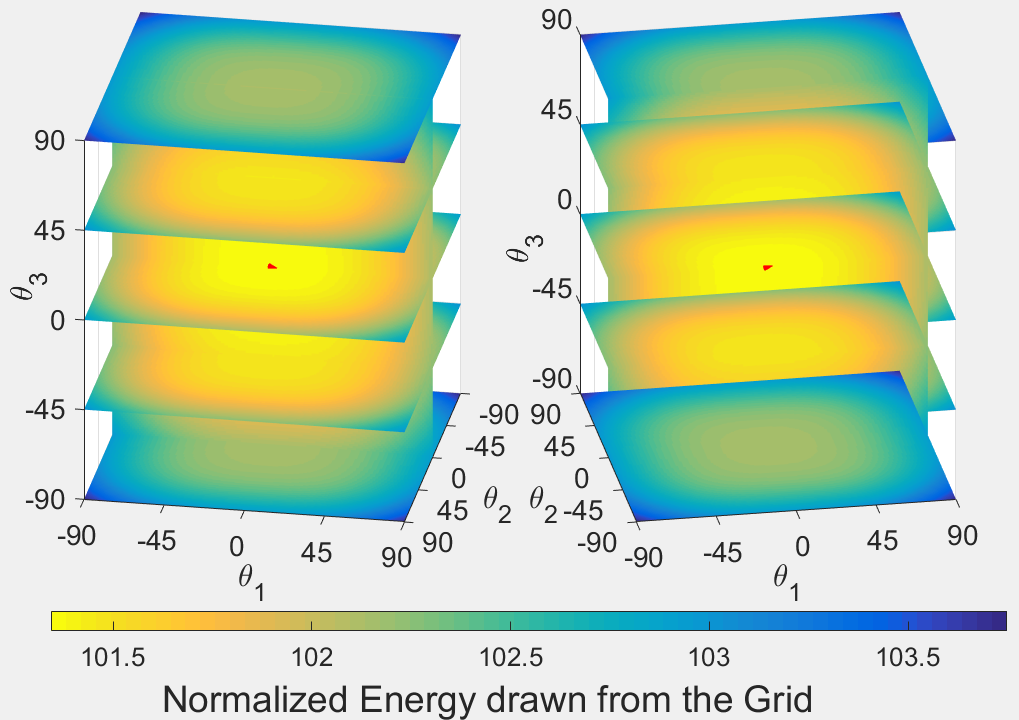
\includegraphics[width=0.34\columnwidth, height=4.6cm]{pictures/results/rein_3PV_scale1_offset1_bis}  & \vspace{0.1cm} 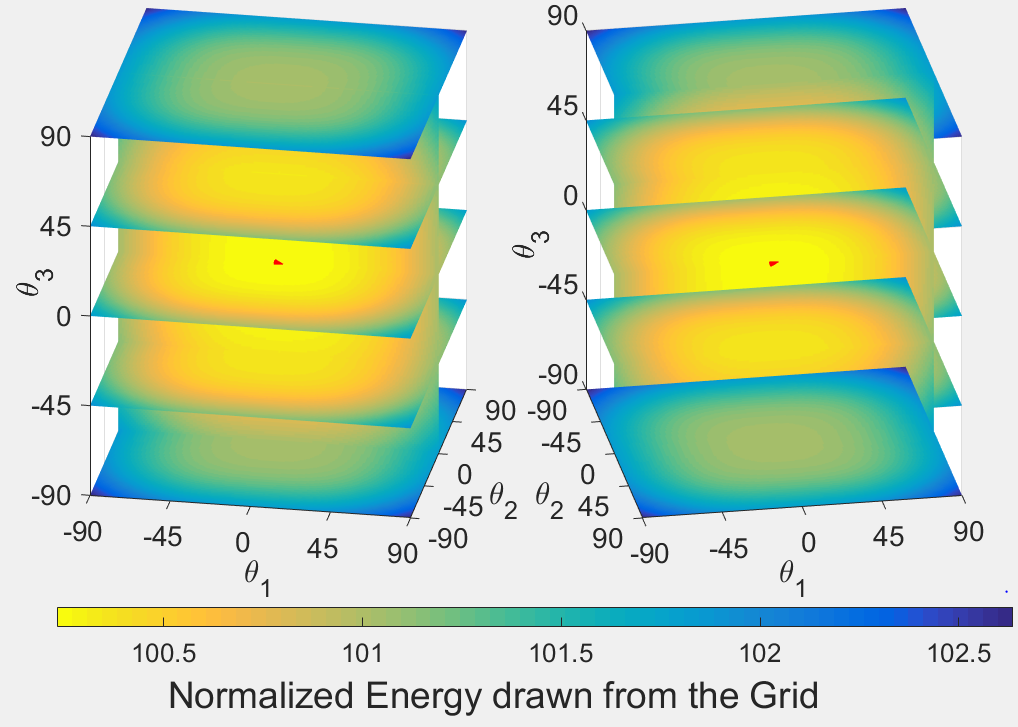
\includegraphics[width=0.34\columnwidth, height=4.6cm]{pictures/results/rein_3PV_scale1_offset1_res} \\
			

						  &   $\quad C(t)= 1$  &   $\quad C(t)=C_{\mathrm{bus}}(t) + 1$ &  $\quad C(t)=C_{\mathrm{res}}(t) + 1$\\  		
							
							 &   (Figure \ref{constant_allgemein} yellow line)  &  (Figure \ref{business_allgemein} yellow line)& (Figure \ref{residential_allgemein} yellow line)\\  \hline 		
				&  Table cell (d): & Table cell (e): &  Table cell (f): \\
						   $G<C$ & \vspace{0.1cm}  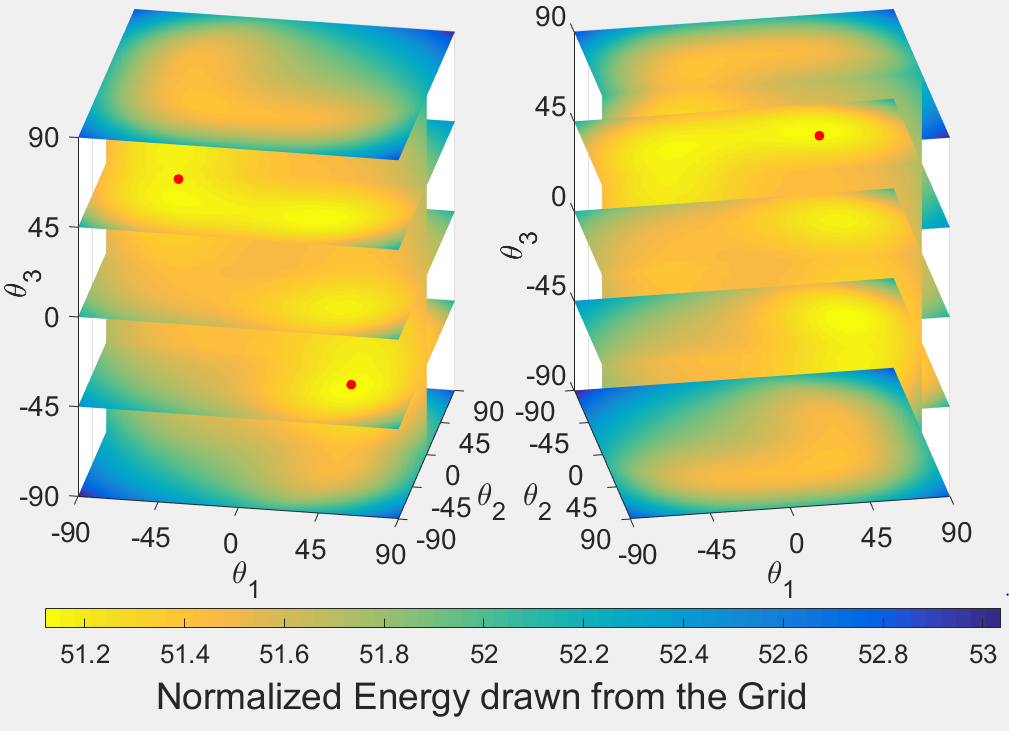
\includegraphics[width=0.34\columnwidth, height=4.6cm]{pictures/results/rein_3PV_scale1_offset0_9_con}  & \vspace{0.1cm} \includegraphics[width=0.34\columnwidth, height=4.6cm]{pictures/results/rein_3PV_scale1_offset0_3_bis}  &
      \vspace{0.1cm} \includegraphics[width=0.34\columnwidth, height=4.6cm]{pictures/results/rein_3PV_scale1_offset0_8_res} \\
		
			&   $\quad C(t)= 0.9$  &  $\quad C(t)=C_{\mathrm{bus}}(t) + 0.3$ &  $\quad C(t)=C_{\mathrm{res}}(t) + 0.8$ \\ 
			
						  &   (Figure \ref{constant_allgemein} green line)&  (Figure \ref{business_allgemein} green line)&  (Figure \ref{residential_allgemein} green line)\\ \hline  
				
				&  Table cell (g): & Table cell (h): &  Table cell (i): \\
				  $G>C$ & \vspace{0.1cm} \includegraphics[width=0.34\columnwidth, height=4.6cm]{pictures/results/rein_3PV_scale1_offset0_8_con}  & \vspace{0.1cm} \includegraphics[width=0.34\columnwidth, height=4.6cm]{pictures/results/rein_3PV_scale1_offset0_bis}         & \vspace{0.1cm} \includegraphics[width=0.34\columnwidth, height=4.6cm]{pictures/results/rein_3PV_scale1_offset0_5_res}\\
			
			&   $\quad C(t)= 0.8$ &   $\quad C(t)=C_{\mathrm{bus}}(t)$  &  $\quad C(t)=C_{\mathrm{res}}(t) + 0.5$ \\  
			
					  &  (Figure \ref{constant_allgemein} gray line)&   (Figure \ref{business_allgemein} gray line)& (Figure \ref{residential_allgemein} gray line)\\  \hline 	
						
						
						&  Table cell (j): & Table cell (k): &  Table cell (l): \\
      $G>>C$ &  \vspace{0.1cm} \includegraphics[width=0.34\columnwidth, height=4.6cm]{pictures/results/rein_3PV_scale1_offset0_6_con}  & \vspace{0.1cm} \includegraphics[width=0.34\columnwidth, height=4.6cm]{pictures/results/rein_3PV_scale0_5_offset0_bis}  &
      \vspace{0.1cm} \includegraphics[width=0.34\columnwidth, height=4.6cm]{pictures/results/rein_3PV_scale1_offset0_res} \\
			
			
				  &   $\quad C(t)= 0.6$&   $\quad C(t)=\frac{1}{2}C_{\mathrm{bus}}(t)$  &  $\quad C(t)=C_{\mathrm{res}}(t) $ \\ 
			
			&\vspace{-0.2cm} (Figure \ref{constant_allgemein} light blue line)& \vspace{-0.2cm}  (Figure \ref{business_allgemein} light blue line)& \vspace{0.3cm}  (Figure \ref{residential_allgemein} light blue line)
		
  \end{tabular}
\end{table}







\newpage



\subsection{Summary of the Key Findings and Discussions of the Results\label{findings}}

To evaluate the effects of different numbers of PV cells, the same consumption profile $C(t)$ is used among corresponding table cells in different tables whenever possible.  For example, the table cell (a) of Table \ref{table_1PV} corresponds to the table cell (a) of Table \ref{table_2PV} and to the table cell (a) of Table \ref{table_3PV}. The comparisons between the different tables are fair because the total surface area $A$ is constant. In other words, there will be no more surface area added by adding another PV cell, instead the total surface area $A$ is divided among $N$ PV cells in each scenario. The only exception is that the table cells (d), (g), and (j) of Table \ref{table_1PV} cannot be compared directly to Table \ref{table_2PV} or Table \ref{table_3PV} because their energy consumption profile $C(t)$ is different. 

From a practical point of view, the optimization algorithm is faster for only a few PV cells (1 or 2 PV cells) than for several PV cells (more than 2 PV cells). In addition, if there are several PV cells with different optimal orientation angles, the spacing between the differently oriented PV cells has to be sufficient enough to avoid shadowing effects on the panels. This increases the area needed for deployment of the PV cells. Furthermore, it is not possible to mount PV cells with different orientation angles on the same array or support structure which increases the material cost for buying several arrays or support structures. Hence, it is recommended to use as less differently oriented PV cells as possible.


If $G << C$ (first rows in Table \ref{opt_1PV}, Table \ref{opt_2PV}, and Table \ref{opt_3PV}), all PV cells should be oriented towards the south, i.e., the optimal orientation angles are $\theta_1^*=\theta_2^*=...=\theta_N^*=0^\mathrm{o}$. If $G << C$, the optimal orientation angles are independent of the shape of the energy consumption profile.

The optimal orientation angles change from south orientation in the $G << C$ scenarios towards the east and/or west orientation in the $G >> C$ scenarios in every column of the Table \ref{table_1PV}, Table \ref{table_2PV}, and Table \ref{table_3PV}. The optimal orientation angles in the $G < C$ scenarios are closer to the south orientation than the east and/or west orientation, whereas the optimal orientation angles in the $G > C$ scenarios are closer to the east and/or west orientation than the south orientation.

The gains of adding the first, second, and third PV cell with optimized orientation angle to the system model 1 are evaluated in the following paragraphs.
\subsubsection{PV Cells with Default Orientation Angles}
The centers of the stripes, squares, and cubes in Table \ref{table_1PV}, Table \ref{table_2PV}, and Table \ref{table_3PV} are the normalized energy drawn
from the main grid, i.e, $f(0^\mathrm{o})$, $f(0^\mathrm{o},0^\mathrm{o})$, and $f(0^\mathrm{o},0^\mathrm{o},0^\mathrm{o})$, if no orientation angle optimization is performed, respectively. PV cells are oriented towards the south in the northern hemisphere by default (cf. Table \ref{over}). $f(0^\mathrm{o})=f(0^\mathrm{o},0^\mathrm{o})=f(0^\mathrm{o},...,0^\mathrm{o})$ if the same consumption profile $C(t)$ is used because the total surface area $A$ in the system model 1 is constant. For example, $f(0^\mathrm{o})$ in Table \ref{table_1PV}(a) equals to $f(0^\mathrm{o},0^\mathrm{o})$ in Table \ref{table_2PV}(a) and $f(0^\mathrm{o},0^\mathrm{o},0^\mathrm{o})$ in Table \ref{table_3PV}(a). 

\subsubsection{Adding the First PV Cell with Optimized Orientation Angle}
A positive (negative) $\Delta_1$ value represents an improvement (deterioration) in performance of the system if the first PV cell is added. 
$\Delta_1>0$ for the table cells (d)-(l) and $\Delta_1=0$ for the table cells (a)-(c) in Table \ref{opt_1PV}. The greatest $\Delta_1$ values for the constant, business, and residential load profiles in Table \ref{opt_1PV} are $0.3829$ (table cell (j)), $2.3318$ (table cell (h)), and $1.5493$ (table cell (l)), respectively. The optimized values $f(\theta_1^*)$ (red lines in Table \ref{table_1PV}) are usually significantly greater than the default values $f(0^\mathrm{o})$ (centers of the stripes in Table \ref{table_1PV}). In other words, orientation angle optimization improves the system performance in most scenarios. $\Delta_1$ is always greater or equal to $0$ because $f(0^\mathrm{o})\geq f(\theta_1^*)$. That means the system performance can only be improved and will never worsen by adding the first PV cell. It should be pointed out that a load profile type can have an optimal orientation angle on the east side ($\theta^*<0^{\mathrm{o}}$), on the west side ($\theta^*>0^{\mathrm{o}}$), as well as oriented southwards ($\theta^*=0^{\mathrm{o}}$) in different scenarios as it can be seen for the residential load profiles (third column) in Table \ref{table_1PV}.

\subsubsection{Adding the Second PV Cell with Optimized Orientation Angle} 
$\Delta_2>0$ for all table cells in Table \ref{opt_2PV} with two optimal points, i.e., (d), (f)-(g), and (i)-(j). $\Delta_2=0$ for all table cells in Table \ref{opt_2PV} with only one optimal point, i.e., (a)-(c), (e), (h), and (k)-(l). The greatest $\Delta_2$ values for the constant, business, and residential load profiles in Table \ref{opt_2PV} are $2.0891$ (table cell (j)), $0$ (table cells (b), (e), (h), and (k)), and $0.5424$ (table cell (i)), respectively. The $\Delta_2$ values are usually smaller than the $\Delta_1$ values for the business and residential load profiles, whereas the $\Delta_2$ values are usually greater than the $\Delta_1$ values for the constant load profiles. Consumption profiles which are similar to the constant profile, e.g., the scenarios in the first column, can often improve their performance (\mbox{$\Delta_2>0$}) by choosing orientation angles with opposite algebraic signs, e.g., $\theta_1^*>0^\mathrm{o}$ and \mbox{$\theta_2^*<0^\mathrm{o}$}, as seen in table cells (d), (g), and (j) in Table \ref{opt_2PV}. Consumption profiles which have significant local maxima in the morning as well as in the afternoon, e.g., the residential load profile scenarios in the third column, can often improve their performance ($\Delta_2>0$) by choosing orientation angles with opposite algebraic signs, e.g., $\theta_1^*>0^\mathrm{o}$ and \mbox{$\theta_2^*<0^\mathrm{o}$}, as seen in table cells (f), and (i) in Table \ref{opt_2PV}. Consumption profiles which have only one significant maximum, e.g., the business load profile scenarios in the second column, cannot improve their performance ($\Delta_2=0$) by adding a second PV cell.

\subsubsection{Adding the Third PV Cell with Optimized Orientation Angle} 
$\Delta_3>0$ for the table cell (l) in Table \ref{opt_3PV}. $\Delta_3=0$ for all table cells in Table \ref{opt_3PV} with only one optimal point, i.e., (a)-(c), (e), (h), and (k). $\Delta_3<0$ for the table cells (d), (f)-(g), and (i)-(j) in Table \ref{opt_3PV}. The greatest and lowest $\Delta_3$ values for the constant, business, and residential load profiles in Table \ref{opt_3PV} are $0$ and $-0.3361$, $0$ and $0$, and $0.1494$ and  $-0.0296$, respectively.
The $\Delta_3$ values are usually smaller than the $\Delta_2$ values and sometimes even negative. That means that adding the third PV cell only improves the system performance slightly in some rare scenarios, whereas the system performance worsens in most other scenarios. 
Consumption profiles which are similar to the constant profile worsen their performance ($\Delta_3<0$) in most scenarios because 3 PV cells cannot equally shift the energy generation peak towards the morning and afternoon hours. Either two PV cells have positive algebraic signs and one PV cell has a negative algebraic sign or the other way around, as seen in table cells (d), (g), and (j) in Table \ref{opt_3PV}. 
Consumption profiles which have two significant local maxima in the morning as well as in the afternoon, e.g., the residential load profile scenarios in the third column, can slightly improve ($\Delta_3>0$) or slightly worsen ($\Delta_3<0$) their performance, as seen in table cells (l), and (i) in Table \ref{opt_3PV}.
Consumption profiles which have only one significant maximum, e.g., the business load profile scenarios in the second column, cannot improve their performance (\mbox{$\Delta_3=0$}) by adding a third PV cell.
In general, consumption profiles which have three significant local maxima between sunrise and sunset or consumption profiles which have two significant local maxima (with one maxima significantly greater than the other one) might benefit in some scenarios from 3 PV cells. But it becomes more and more difficult to find such specific consumption profiles and scenarios to justify that 3 or more PV cells are necessary to improve the system performance significantly.



\section{Summary of Chapter \ref{Chapter_1}\label{sum_Chapter_1}}
In Chapter \ref{Chapter_1}, the orientation angles of $N$ PV cells powering one BS were jointly optimized to improve the match between the two profiles on a daily timescale. The energy generation profiles of randomly inclined and oriented PV cells were analytically derived by the irradiance values received at a horizontally-mounted PV cell at the same location. The energy drawn per day from the main grid by the BS given its energy consumption profile was used as the performance metric to determine the optimal set of orientation angels.
The main results are that the system performance ($\Delta_1 > 0$) can be increased significantly by deploying one PV cell with optimal orientation angel $\theta_1^*$ (or several PV cells with the same orientation angle $\theta_1^*$) if the energy generation of the PV cell is slightly smaller ($G<C$), is slightly greater ($G>C$), or is significantly greater ($G>>C$) than the energy consumption of the BS. This is caused by the ability to shift the energy generation peak from noon towards the most significant local maximum between sunrise and sunset of the energy consumption profile. 
Furthermore, the system performance ($\Delta_2 > 0$) can be further increased by deploying two PV cells with jointly optimized orientation angles $\theta_1^*$ and $\theta_2^*$ (or several PV cells where half of them are deployed with $\theta_1^*$ and the other half with $\theta_2^*$) if a constant energy consumption profile or a consumption profile with significant local maxima in the morning as well as in the afternoon are given. This is caused by the ability to shift the energy generation peak from noon towards the morning with east-oriented PV cells, while the other west-oriented PV cells shift the energy generation peak towards the afternoon in the northern hemisphere. Because there are only two directions (morning and afternoon) that the energy can be shifted to, the system performance can not be further increased significantly by deploying more than 2 differently oriented PV cells. More than 2 differently oriented PV cells may even degrade the system performance ($\Delta_3 < 0$) in some scenarios.



\clearpage
\chapter{Impact of the Battery Capacity on the Optimal Orientation Angle of a PV Cell\label{Chapter_2}}
\settablecounter{3}{1}


Chapter \ref{Chapter_2} will extend the system model in Chapter \ref{Chapter_1} by adding a battery to the BS. The battery is modeled by a Markov chain in this chapter. The system model in Chapter \ref{Chapter_1} has no batteries deployed at the BS. Nonetheless, Chapter \ref{Chapter_1} can be seen as special case of Chapter \ref{Chapter_2} because the batteries can have a battery capacity of $0$ in the system model of Chapter \ref{Chapter_2}.



\section{Literature Review: Batteries at BSs}


It has been shown that the resiliency of cellular networks in disaster events, such as earthquakes and hurricanes, is higher if the energy mix of the cellular networks includes harvest renewable energy instead of relying solely on the power from the main grid \cite{Kwasinski2013LessonsFF}. The service of the cellular network usually breaks down during a disaster event because power lines are damaged and the BSs run out of energy. In addition, back-up generators rely on petrol, which has to be transported to the sites of the BSs via roads, which are often damaged as well in disaster events. Because the cellular network service is so vital during a disaster event to coordinate rescue missions, police operations, and military operations, the cellular network is required to be operational 99.999\% of the time during a year, whereas the power grid is required to be operational only 99.9\% in the U.S. \cite{residential}. In other words, the total yearly outage time of the power grid is less than nine hours, whereas the requirements for cellular networks is much higher than that. Because power grids have lower reliability requirements than that of cellular networks, BSs are typically equipped with batteries that last for a few hours. The capacity of the batteries is usually around four hours but can be higher for some BSs as well \cite{residential}.

PV cells have a very strong diurnal cycle. \cite{CHATTOPADHYAY2017176,RasmussenMortenGrud2012Sabs} showed that a storage capacity of six hours of the average consumption of the appliance is sufficient to smoothen the diurnal cycle of the PV cells. In scenarios where only solar energy is harvested and no other energy sources are available, a storage capacity of twelve hours was recommended by \cite{CHATTOPADHYAY2017176,RasmussenMortenGrud2012Sabs}.


A life cycle energy cost assessment at a stand-alone PV system was conducted in \cite{Thiaux2010602} to evaluate the long term benefits of shifting the energy consumption profile towards the energy generation profile. A better match of both profiles led to a longer battery lifetime due to less battery charging-discharging cycles and the opportunities to downsize the battery capacity and PV cell surface area. 



A good match between the energy generation profile of the PV cell and the energy consumption profile of the BS can be achieved by either installing a small battery (or no battery) with orientation angle optimization or installing a large battery without orientation angle optimization. Nonetheless, batteries are expensive (25 - 250\euro, 220\euro{} and 1500\euro{} per kWh for the battery types Lead-Acid, NaS and Li-Ion, respectively \cite{RUDOLF2013139}) and have a short lifetime (3 - 9 years \cite{CROSSLAND201530}) compared with the warranty lifetimes of PV cells (PV cell manufacturers guarantee a 80\% system performance warranty for around 20 years \cite{6745088}). Therefore, battery replacements significantly contribute to the system lifetime cost \cite{CROSSLAND201530}. Small batteries with orientation angle optimization are practically the more cost-effective option compared with large batteries without orientation angle optimization.


Markov chain models have been used in the literature to model batteries, as seen in \cite{ParzyszFanny2017PCAf, SakrAhmedHamdi2015AoKU,TingwuWang2016ASiS}.


\section{Contributions of Chapter \ref{Chapter_2}}
The contributions of Chapter \ref{Chapter_2} are summarized as follows:

\begin {itemize}

\item Developing a PV cell's orientation angle optimization algorithm with Markov chain based battery model of a solar-powered BS with battery. The algorithm takes into account the battery capacity and the energy consumption profile of the BS. The number of user equipments (UEs) served by the BS throughout the day $\overline{S_{\mathrm{UE}}}(\theta)$ is used as the performance metric to identify the optimal orientation angle.
\item Verifying the accuracy of the proposed algorithm by showing that simulation trials converge based on the law of large numbers to 
the output $\overline{S_{\mathrm{UE}}}(\theta)$ of the proposed algorithm. 
\item Showing that the proposed algorithm (depends on the number of battery states) requires a shorter running time than the simulation trials (depends on the number of trials) for moderate battery state resolutions.
\item Investigating the dependency of the optimal PV cell orientation angle on the given battery capacity.
\end {itemize}

\section{System Model 2 - One PV Cell Powering a BS with Battery\label{system_2}}






Figure  \ref{ene2} depicts the system model 2 considered in this chapter. It consists of an energy generation part with one PV cell, an energy storage part made of a battery, and an energy consumption part composed of a BS. The energy flow follows the arrows in Figure  \ref{ene2} and can only be altered by choosing different orientation angles for the PV cell. All other parameters will be fixed. The energy generation flow is denoted by $G_{\theta,1}(t)$ in Figure \ref{ene2}. The energy consumption flow is divided in a load-independent part, denoted by $c_{\mathrm{con}}$, and a load-dependent part, denoted by $c_\theta(t)$, in Figure \ref{ene2}.

\begin{figure}[H]
	\centering	
		\includegraphics[width=1\columnwidth]{pictures/qq}
\caption{Illustration of system model 2\label{ene2}}
\end{figure}

\subsection{Solar Energy Storage Model}
The BS is only powered by a PV cell. The only controllable parameter in the system model 2 is the PV cell orientation angle. The day is divided into $T$ time steps. The index of a time step is denoted by $t \in \{1,...,T\}$.
Each time step has three distinguish flows, first the energy generation flow will be executed followed by the load-independent energy consumption flow and then the load-dependent energy consumption flow (cf. Figure \ref{ene2}). During the energy generation flow, the amount of generated energy in this time step is calculated and stored in the battery. During the energy consumption flows, the amount of consumed energy by the BS in this time step is subtracted from the battery. In reality all three periods occur simultaneously. For applications that require a simultaneous energy generation and consumption, the length of the time steps can be chosen small enough to achieve a nearly simultaneous energy generation and consumption. 





\subsection{Energy Generation Flow and Load-independent Energy Consumption Flow}\label{energy}


The formula for the normalized energy generated by one PV cell deployed with orientation angle $\theta$ at time step $t$, denoted by $G_{\theta,1}(t)$, has been derived in Chapter \ref{Chapter_1} and can be calculated by (\ref{norma}). 


The battery has an upper bound and a lower bound that determine how much of the generated energy $G_{\theta,1}(t)$ can be stored in the battery. In addition, the load-independent energy consumption of the BS, denoted by $c_{\mathrm{con}}$, has to be subtracted from the battery at the beginning of each time step. 


The available energy, denoted by $a_{\theta}(t)$, in the battery at time step $t$ is as follows:


\begin{equation}\label{available}
a_{\theta}(t)=\max\{0,\min\{b_\theta(t-1)+G_{\theta,1}(t)-c_{\mathrm{con}},b_{\max}\}\},
\end{equation}
\noindent
where $b_{\theta}(t-1)$ is the stored energy in the battery in time step $t-1$, $c_{\mathrm{con}}$ is the load-independent energy consumption of the BS during one time step, and $b_{\max}$ is the maximum battery capacity. The min in (\ref{available}) ensures that the stored energy in the battery is less or equal the maximum battery capacity. The max in (\ref{available}) ensures that the stored energy in the battery is greater or equal $0$. 

The amount of energy stored in the battery at time step $0$ is $b_{\mathrm{begin}}$ as follows:
\begin{equation}
 b_{\theta}(0)=b_{\mathrm{begin}}.
\end{equation}


\subsection{Load-dependent Energy Consumption Flow}\label{traffic}

To model the temporal fluctuation of the BS's energy consumption, the number of user equipments (UEs) connected to the BS at time step $t$ is modeled by a random variable $l(t)$, which follows a Poisson distribution (PD) with density parameter $\lambda(t)$. The number of UEs in the coverage area of a BS is commonly modeled as a Poisson point process in the literature \cite{poisson, baccell00403039, NET-015}. Hence, $l(t)$ is as follows:

\begin{equation}
\label{PPP1}
l(t):=\mathrm{PD}(\lambda(t)).
\end{equation}
Without loss of generality, it is assumed that the BS is located in a business-area. The traffic load profile of a BS in a business-area, denoted by $C_{\mathrm{bus}}(t)$, has been derived in Chapter \ref{Chapter_1} and is given in Figure \ref{all_consumption_profiles}. Nonetheless, the analysis can be applied to any other location and traffic load profile as well.
 Hence, the density parameter $\lambda(t)$ is as follows:

\begin{equation}
\label{P}
\lambda(t)= C_{\mathrm{bus}}(t).
\end{equation}



The number of served UEs\footnote{UEs that cannot be served by the BS due to a lack of renewable stored energy in the battery might be off-loaded to other BSs or the BS uses main grid energy to serve these UEs. Only UEs which are served by the available renewable energy will be counted by $s_\theta(t)$.} by the BS at time step $t$, denoted by $s_\theta(t)$, is limited either by the number of UEs connected to the BS or the available energy as follows:


\begin{equation}
\label{PPP2}
s_\theta(t)=\min\Big\{l(t),\Big\lfloor \frac{a_\theta(t)}{c_{\mathrm{UE}}}\Big\rfloor\Big\},
\end{equation}



\noindent
where $a_{\theta}(t)$ is the available energy at time step $t$, and $c_{\mathrm{UE}}$ is the average amount of energy needed to serve one UE.

The load-dependent energy consumption $c_\theta(t)$ of the BS in time step $t$ is given by


\begin{equation}
\label{PPP3}
c_\theta(t)=s_\theta(t)\cdot c_{\mathrm{UE}}.
\end{equation}



 The residual energy in the battery at the end of time step $t$ can be calculated by

\begin{equation}
\label{bat}
b_\theta(t)=a_\theta(t)-c_\theta(t).
\end{equation}

\subsection{Determination of the Average Number of Served UEs}
Eq. (\ref{PPP2}) ensures that the consumed energy by the BS is less than or equal to the stored energy in the battery. As a result, it is possible that some UEs cannot be served\footnote{UEs that cannot be served by the BS due to a lack of renewable stored energy might be off-loaded to other BSs or the BS uses main grid energy to serve these UEs. Only UEs which are served by the available renewable stored energy will be counted by $s_\theta(t)$.} by the BS due to a lack of renewable stored energy. Therefore, the number of served UEs $S_{\mathrm{UE}}(\theta)$ throughout the day by a PV cell with orientation angle $\theta$ is used as the performance metric, where $S_{\mathrm{UE}}(\theta)$ is as follows:

\begin{equation}
\label{PPP}
S_{\mathrm{UE}}(\theta)=\sum_{t=1}^{T} s_\theta(t).
\end{equation}

Because the $l(t)$ values are random variables, $\overline{S_{\mathrm{UE}}}(\theta)$ denotes the average value of $S_{\mathrm{UE}}(\theta)$.



The orientation angle $\theta$ which achieves the highest $\overline{S_{\mathrm{UE}}}(\theta)$ value is considered as optimal orientation angle $\theta^*$ as follows:

\begin{equation}
\label{sol}
\theta^* =\mathrm{arg} \enskip \mathrm{max}_{\theta} \enskip\overline{S_{\mathrm{UE}}}(\theta).
\end{equation}





\section{Orientation Angle Optimization Algorithm with Markov Chain Based Battery\label{jj}}
The following PV cell's orientation angle optimization algorithm with Markov chain based battery model (Algorithm \ref{mar}) can efficiently determine the optimal orientation angle of the PV cell at a BS with battery. To show the effectiveness of the proposed algorithm, a simulation algorithm (Algorithm \ref{sim}) will be developed in the Section \ref{see} as well. The advantages of the proposed algorithm in comparison with the simulation algorithm (Algorithm \ref{sim}) with respect to accuracy and running time will be evaluated in Section \ref{results_system_2}.

All energy values are discretized with a precision of $\mu$, i.e., $\tilde{G}_{\theta,1}(t)$ will be the closest multiple of $\mu$ from $G_{\theta,1}(t)$. For example, if $\mu=\frac{1}{1000}$, and $G_{\theta,1}(t)=1.2756$, then $\tilde{G}_{\theta,1}(t)=1.276$.


There are $S_{\mathrm{max}}=\frac{b_{\max}}{\mu}+1$ battery energy states. The battery energy states $0, 1, 2, 3, ...,$ and $\frac{b_{\max}}{\mu}$ represent $0, \mu, 2\cdot\mu, 3\cdot\mu, ...,$ and $b_{\max}$ units of normalized energy, respectively. Without loss of generality, $b_{\mathrm{begin}}$, $b_{\max}$, $c_{\mathrm{UE}}$, and $c_{\mathrm{con}}$ are multiple of $\mu$.

 The expression $\mathbb{P}(a_{\theta}(t)=i)=x$ means that the probability of having $i$ units of normalized energy available in the battery at the beginning of time step $t$ is $x$. The expression $\mathbb{P}(b_{\theta}(t)=i)=x$ means that the probability of the battery having stored $i$ units of normalized energy at the end of time step $t$ is $x$.


The following subsections will go through the Algorithm \ref{mar} line by line. The expression $\lfloor x \rfloor$ means that the variable $x$ is rounded down to the nearest integer value.


\subsection{Markov Chain Initialization\label{Tet}}



Because $l(t)$ is a Poisson distributed random variable, $\mathbb{P}(l(t)= r)$, and $\mathbb{P}(l(t)\geq r)$ are $\frac{\lambda(t)^r \cdot e^{-\lambda(t)}}{r!}$, and $1 - \sum_{w=0}^{r-1}\frac{\lambda(t)^w\cdot e^{-\lambda(t)}}{w!}$, respectively \cite{poisson_formula} (Algorithm \ref{mar} line: \ref{in1} - \ref{in2}). 

$S_{\mathrm{max}}$ is initialized (Algorithm \ref{mar} line: \ref{battery_stages}).
The initial battery state $b_\theta(0)$ is equal to $b_{\mathrm{begin}}$ at the beginning of Algorithm \ref{mar}. Therefore, the probability of the battery state being $b_{\mathrm{begin}}$ at time step $0$ is $1$, whereas all the other battery states have a probability of $0$ (Algorithm \ref{mar} line: \ref{ini1_mar} - \ref{ini2_mar}). There are no UEs served at the beginning of Algorithm \ref{mar} (Algorithm \ref{mar} line: \ref{sss}).
Eq. (\ref{P}) is used to calculate the UE density parameters $\lambda(t)$ for all time steps (Algorithm \ref{mar} line: \ref{c_mar}). 

\subsection{Energy Generation Flow and Load-independent Energy Consumption Flow of Algorithm \ref{mar}}

All $\mathbb{P}(a_\theta(t)=i)$ values are set at $0$ at the beginning (Algorithm \ref{mar} line: \ref{a_ini}).
If the battery is in state $i$, $S_{\mathrm{Shift}}$ calculates the new battery state after the generated energy $\tilde{G}_{\theta,1}(t)$ is added to the battery and the load-independent energy consumption of the BS $c_{\mathrm{con}}$ is subtracted from the battery (Algorithm \ref{mar} line: \ref{she}). $S_{\mathrm{Shift}}$ takes into account the upper bound and the lower bound of the battery (Algorithm \ref{mar} line: \ref{she}).
If $\tilde{G}_{\theta,1}(t)>c_{\mathrm{con}}$, then every battery state increases by $\frac{\tilde{G}_{\theta,1}(t)-c_{\mathrm{con}}}{\mu}$ battery states or reaches the maximum battery state $S_{\mathrm{max}}-1$ if it comes to a battery overflow. This is depicted in Figure \ref{fig:gener}.
If $\tilde{G}_{\theta,1}(t)<c_{\mathrm{con}}$, then every battery state decreases by $\frac{c_{\mathrm{con}}-\tilde{G}_{\theta,1}(t)}{\mu}$ battery states or reaches the minimum battery state $0$ if the battery depletes. This is depicted in Figure \ref{fig:gener2}.
If $\tilde{G}_{\theta,1}(t)=c_{\mathrm{con}}$, there is no energy added or subtracted from the battery.
Each transition occurs with a probability of $1$, which is depicted on top of each arrow in Figures \ref{fig:gener} - \ref{fig:gener2}.

The probability of the battery state being $i$ at the time step $t-1$, i.e., $\mathbb{P}(b_\theta(t-1)=i)$, is added to the probability of the new battery state, i.e., $\mathbb{P}(a_\theta(t)=S_{\mathrm{Shift}})$ (Algorithm \ref{mar} line: \ref{shift}).






\begin{figure}[H]
	\centering
		\includegraphics[scale=0.6]{pictures/1}
	\caption{Energy generation flow and load-independent energy consumption flow if $\tilde{G}_{\theta,1}(t)>c_{\mathrm{con}}$\label{fig:gener}}
\end{figure}

\begin{figure}[H]
	\centering
		\includegraphics[scale=0.6]{pictures/EN}
	\caption{Energy generation flow and load-independent energy consumption flow if $\tilde{G}_{\theta,1}(t)<c_{\mathrm{con}}$\label{fig:gener2}}
\end{figure}




\subsection{Load-dependent Energy Consumption Flow of Algorithm \ref{mar}}
The number of UEs in the coverage area of the BS, denoted by $l(t)$, is Poisson distributed with density parameter $\lambda(t)$, i.e., $l(t):= \mathrm{PD}(\lambda(t))$. The probability of $l(t)$ to be equal to an integer value $r$, denoted by $\mathbb{P}(l(t)=r)$, is given for a Poisson distribution by $\frac{\lambda(t)^r \cdot e^{-\lambda(t)}}{r!}$ \cite{poisson_formula} (Algorithm \ref{mar} line: \ref{in1}). The expression $\mathbb{P}(l(t)\geq r)$ is given for a Poisson distribution by $1 - \sum_{w=0}^{r-1}\frac{\lambda(t)^w\cdot e^{-\lambda(t)}}{w!}$ \cite{poisson_formula} (Algorithm \ref{mar} line: \ref{in2}).

Each served UE consumes $c_{\mathrm{UE}}$ units of normalized energy in each time step. Therefore, every battery state has to be decreased by $\frac{c_{\mathrm{UE}}}{\mu}$ battery states for every served UE in each time step.

This paragraph derives the update formulas for the battery states from $\frac{c_{\mathrm{UE}}}{\mu}$ to $S_{\max}-1$ (Algorithm \ref{mar} line: \ref{c11} - \ref{c12}). Figure \ref{fig:consum1} shows only the incoming arrows for the battery state $\frac{c_{\mathrm{UE}}}{\mu}$ as an example. The battery state $i \in \{\frac{c_{\mathrm{UE}}}{\mu},...,S_{\max}-1\}$ has $\Big\lfloor \frac{(S_{\max}-1-i)\cdot\mu}{c_{\mathrm{UE}}} \Big\rfloor + 1 $ incoming arrows. $r \in \big\{0,...,\Big\lfloor\frac{(S_{\max}-1-i)\cdot\mu}{c_{\mathrm{UE}}}\Big\rfloor\big\}$ describes the transition from battery state $i+r \cdot \frac{c_{\mathrm{UE}}}{\mu}$ to battery state $i$ when exactly $r$ UEs are served. The transition probability is $\mathbb{P}(l(t)=r) $ for this transition which is depicted next to the transition arrow in Figure \ref{fig:consum1}.

This paragraph derives the update formulas for the battery states from $0$ to $\frac{c_{\mathrm{UE}}}{\mu}-1$ (Algorithm \ref{mar} line: \ref{c21} - \ref{c22}). Figure \ref{fig:consum2} shows only the incoming arrows for the battery state $0$ as an example. The battery state $i \in \{0,...,\frac{c_{\mathrm{UE}}}{\mu}-1\}$ has $\Big\lfloor \frac{(S_{\max}-1-i)\cdot\mu}{c_{\mathrm{UE}}} \Big\rfloor + 1 $ incoming arrows. $r \in \big\{0,...,\Big\lfloor \frac{(S_{\max}-1-i)\cdot\mu}{c_{\mathrm{UE}}} \Big\rfloor\big\}$ describes the transition from battery state $i+r \cdot \frac{c_{\mathrm{UE}}}{\mu}$ to battery state $i$ when more than $r-1$ UEs are in the coverage area of the BS, which means the BS can only serve $r$ UEs and the remaining UEs cannot be served due to the lack of available renewable stored energy. The transition probability is $\mathbb{P}(l(t)\geq r) $ for this transition which is depicted next to the transition arrow in Figure \ref{fig:consum2}.



\begin{figure}[H]
	\centering
		\includegraphics[scale=0.6]{pictures/33}
	\caption{Energy consumption flow for the battery state $\frac{c_{\mathrm{UE}}}{\mu}$ \label{fig:consum1}}
\end{figure}


\begin{figure}[H]
	\centering
		\includegraphics[scale=0.6]{pictures/rr}
	\caption{Energy consumption flow for the battery state $0$ \label{fig:consum2}}
\end{figure}


\subsection{Determination of the Average Number of Served UEs of Algorithm \ref{mar}}
When the battery is in state $i$, it can serve $r \in \{0,...,\Big\lfloor \frac{i\cdot\mu}{c_{\mathrm{UE}}} \Big\rfloor\}$ UEs. When $r\in\{0,...,\Big\lfloor \frac{i\cdot\mu}{c_{\mathrm{UE}}} \Big\rfloor   -1\}$, the energy in the battery is decreased from battery state $i$ with the transition probability of $\mathbb{P}(l(t)=r)$. Exactly $r$ UEs were served, that is why the expression in Algorithm \ref{mar} line: \ref{hi1} is multiplied by $r$. When $r= \Big\lfloor \frac{i\cdot\mu}{c_{\mathrm{UE}}} \Big\rfloor$, the energy in the battery is decreased from battery state $i$ with the transition probability of $\mathbb{P}(l(t)\geq \Big\lfloor \frac{i\cdot\mu}{c_{\mathrm{UE}}} \Big\rfloor) $. Exactly $\Big\lfloor \frac{i\cdot\mu}{c_{\mathrm{UE}}} \Big\rfloor$ UEs were served, that is why the expression in Algorithm \ref{mar} line: \ref{hi2} is multiplied by $\Big\lfloor \frac{i\cdot\mu}{c_{\mathrm{UE}}} \Big\rfloor$. 



The PV cell's orientation angle optimization algorithm with Markov chain based battery model is summarized as follows:


\begin{breakablealgorithm}                
\caption{\textbf{Algorithm 1: } PV cell's orientation angle optimization algorithm with Markov chain based battery model\label{mar}}   \singlespacing                       
\begin{algorithmic} [1]                 
    \Require $\gamma$, $\mu$, $T$, $b_{\mathrm{begin}}$, $b_{\max}$, $c_{\mathrm{con}}$, $c_{\mathrm{UE}}$, $\tilde{G}_{\theta,1}(t) \enskip \forall t\enskip\forall \theta  \text{, and } C_{\mathrm{bus}}(t) \enskip \forall t$  
   \Ensure $\theta^*$
	\State \% $\mathbb{P}(l(t)=r)=\frac{\lambda(t)^r \cdot e^{-\lambda(t)}}{r!}$ \label{in1}
	\State \% $\mathbb{P}(l(t)\geq r)=1 - \sum_{w=0}^{r-1}\frac{\lambda(t)^w\cdot e^{-\lambda(t)}}{w!}$ \label{in2}
	\item[]
	\For{all $\theta\in \{-40^{\mathrm{o}},-35^{\mathrm{o}},...,90^{\mathrm{o}}\}$}
	\item[]
	\State \text{ \% Initialization} \label{ini1} 		
	\State $S_{\mathrm{max}}=\frac{b_{\max}}{\mu}+1$\label{battery_stages}
		\State $\mathbb{P}(b_\theta(0)=\frac{b_{\mathrm{begin}}}{ \mu})=1$ \label{ini1_mar}
\State $\mathbb{P}(b_\theta(0)=i)=0 \quad \quad \quad \forall i \in \{0,...,S_{\mathrm{max}}-1\} \setminus  (\frac{b_{\mathrm{begin}}}{ \mu})$ \label{ini2_mar}
\State $\overline{S_{\mathrm{UE}}}(\theta)=0$\label{sss}
	\For{$t=1:T$}
		\State $\lambda(t)=C_{\mathrm{bus}}(t) $\label{c_mar}
	\EndFor
		\item[]

		
\For{$t=1:T$}
		\State \text{ \% Energy generation flow and load-independent energy consumption flow}\label{gen1}  
		
	\State $\mathbb{P}(a_\theta(t)=i)=0\quad \quad \quad\quad \quad \forall i \in \{0,...,S_{\mathrm{max}}-1\}\quad$ \text{ \% Initialization}\label{a_ini}
		\For{$i \in \{0,...,S_{\mathrm{max}}-1\}$}
		
		\State $S_{\mathrm{Shift}}=\max\{0,\min\{i+\frac{\tilde{G}_{\theta,1}(t)-c_{\mathrm{con}}}{\mu},\frac{b_{\mathrm{max}}}{\mu}\}\}$\label{she}
		\State $\mathbb{P}(a_\theta(t)=S_{\mathrm{Shift}})=\mathbb{P}(a_\theta(t)=S_{\mathrm{Shift}})+\mathbb{P}(b_\theta(t-1)=i)$\label{shift}
		\EndFor
		
		\item[]
		\State \text{ \% Adding the average number of UEs served at time step $t$ to $\overline{S_{\mathrm{UE}}}(\theta)$}
    \For {$i=0:S_{\mathrm{max}}-1$}
     \For {$r=0: \lfloor \frac{i\cdot \mu}{c_{\mathrm{UE}}} \rfloor   -1$}
    \State $\overline{S_{\mathrm{UE}}}(\theta)=\overline{S_{\mathrm{UE}}}(\theta)+ r \cdot \mathbb{P}(l(t)=r) \cdot \mathbb{P}(a_\theta(t)=i) $ \label{hi1}
       \EndFor
   \State      $\overline{S_{\mathrm{UE}}}(\theta)=\overline{S_{\mathrm{UE}}}(\theta)+ \lfloor \frac{i \cdot \mu}{c_{\mathrm{UE}}} \rfloor \cdot \mathbb{P}(l(t)\geq \lfloor \frac{i\cdot \mu}{c_{\mathrm{UE}}} \rfloor ) \cdot \mathbb{P}(a_\theta(t)=i) $\label{hi2}   
       \EndFor 
		\item[]
			\State \text{ \% Load-dependent energy consumption flow} \label{con1} 
			\State $\mathbb{P}(b_\theta(t)=i)=\sum_{r=0}^{ \Big\lfloor \frac{(S_{\mathrm{max}}-1-i)\cdot \mu}{c_{\mathrm{UE}}} \Big\rfloor } \Big(  \mathbb{P}(l(t)\geq r) \cdot \mathbb{P}(a_\theta(t)=i +r \cdot \frac{c_{\mathrm{UE}}}{\mu})\Big) $\label{c21}  
			
		\State $	\quad \forall i \in \{0,...,\frac{c_{\mathrm{UE}}}{\mu}-1\}$ \label{c22}  
    \State $\mathbb{P}(b_\theta(t)=i)=\sum_{r=0}^{ \Big\lfloor \frac{(S_{\mathrm{max}}-1-i)\cdot \mu}{c_{\mathrm{UE}}} \Big\rfloor }  \Big( \mathbb{P}(l(t)=r)  \cdot\mathbb{P}(a_\theta(t)=i +r \cdot \frac{c_{\mathrm{UE}}}{\mu})\Big)$\label{c11}  
	\State 	$\quad \enskip\!\! \forall i \in \{\frac{c_{\mathrm{UE}}}{\mu},...,S_{\mathrm{max}}-1\}$ \label{c12}  
\EndFor
\EndFor
\Return $\theta^*=\arg \displaystyle\max_{\theta\in[-90^{\mathrm{o}},90^{\mathrm{o}}]} \overline{S_{\mathrm{UE}}}(\theta)$
\end{algorithmic}
\end{breakablealgorithm}




\section{Derivation of a Simulation Algorithm as Baseline \label{see}}

Eqs. (\ref{available}) - (\ref{sol}) are used to derive the following simulation algorithm (Algorithm \ref{sim}). Algorithm \ref{sim} is the baseline for the performance comparison with the shown proposed algorithm (Algorithm \ref{mar}).


 



\begin{algorithm} [H]                     
\caption{Simulation algorithm\label{sim}}     
\label{alg2}                    
\begin{algorithmic} [1] 
          
    \Require $\gamma$, $L$, $T$, $b_{\mathrm{begin}}$, $b_{\max}$, $c_{\mathrm{con}}$, $c_{\mathrm{UE}}$, $G_{\theta,1}(t) \enskip \forall t\enskip\forall \theta  \text{, and } C_{\mathrm{bus}}(t) \enskip \forall t$  
   \Ensure $\theta^*$
		\For{all $\theta\in \{-40^{\mathrm{o}},-35^{\mathrm{o}},...,90^{\mathrm{o}}\}$}
	\item[]
	   \State  $\overline{S_{\mathrm{UE}}}(\theta)=0$
				\For{$l=1:L$}
				\item[]
					\State \text{\% Initialization} 
\State $b_\theta(0)=b_{\mathrm{begin}}\quad$
		\For{$t=1:T$}
							\State \text{\% Energy generation flow}
        \State $a_\theta(t)=\max\{0,\min\{b_\theta(t-1)+G_{\theta,1}(t)-c_{\mathrm{con}},b_{\max}\}\}$ \label{h_sim}
			\item[]
			\State \text{\% Energy consumption flow} 
			\State $\lambda(t)=C_{\mathrm{bus}}(t)$  \label{c_sim}
			\State	$s_\theta(t)=\min\{\mathrm{PD}(\lambda(t)),\lfloor \frac{a_\theta(t)}{c_{\mathrm{UE}}}\rfloor\}$,
	\State $b_\theta(t)=a_\theta(t)-s_\theta(t)\cdot c_{\mathrm{UE}}$ 
		\EndFor
		

		\State $\overline{S_{\mathrm{UE}}}(\theta)=\overline{S_{\mathrm{UE}}}(\theta)+\sum_{t=1}^{T} s_\theta(t)$
		\EndFor 			 
\State $\overline{S_{\mathrm{UE}}}(\theta)= \overline{S_{\mathrm{UE}}}(\theta)/L$
\EndFor
		\Return $\theta^*=\arg \displaystyle\max_{\theta\in[-90^{\mathrm{o}},90^{\mathrm{o}}]} \overline{S_{\mathrm{UE}}}(\theta)$
\end{algorithmic}
\end{algorithm}


The simulation algorithm (Algorithm \ref{sim}) has to be run for a large number $L$ until the average of the $S_{\mathrm{UE}}(\theta)$ value converges to a fixed value, denoted by $\overline{S_{\mathrm{UE}}}(\theta)$. 

\section{Results and Discussion\label{results_system_2}}



\subsection{Running Time of the proposed Algorithm and the Simulation Algorithm\label{n}}
The simulation algorithm has a running time of $\mathcal{O}(L \cdot T)$, whereas the proposed algorithm has a running time of $\mathcal{O}(S_{\max}^2 \cdot T)$. Therefore, the proposed algorithm outperforms the simulation algorithm when the battery is not divided into too many battery states $S_{\max}$. Especially for small BSs with small battery capacities, the proposed algorithm is an effective tool to determine the optimal PV cell orientation. 


\subsection{Accuracy of the Proposed Algorithm and the Simulation Algorithm \label{anna}}
The proposed algorithm has the advantage that it can generate the exact $\overline{S_{\mathrm{UE}}}(\theta)$ value, whereas the simulation algorithm only converges to the $\overline{S_{\mathrm{UE}}}(\theta)$ value.
The parameters in Table \ref{frog} are used for the simulation algorithm and the proposed algorithm. Both algorithms are run for every orientation angle $\theta \in \{-40^{\mathrm{o}},-35^{\mathrm{o}},...,85^{\mathrm{o}},90^{\mathrm{o}}\}$ with constant inclination angle $\gamma=36^{\mathrm{o}}$ (optimal inclination angle for Greenwich (London, UK) in summer). The simulation algorithm is run $L=100000$ times to achieve a good convergence. 





\begin{longtable}{@{}l*{2}{|l}l@{}}
\caption{\\ Input parameters of system model 2\label{frog}}\\ \toprule
\textbf{Parameter}	&\textbf{Description}				&  \textbf{Value} \\ \midrule
$\theta$  & Orientation angle of PV cell&$\in \{-40^{\mathrm{o}},-35^{\mathrm{o}},...,90^{\mathrm{o}}\}$  \\
$\theta^*$  & Optimal orientation angle of PV cell&$\in \{-40^{\mathrm{o}},-35^{\mathrm{o}},...,90^{\mathrm{o}}\}$  \\
$\gamma$ & Inclination angle of PV cell& $36^{\mathrm{o}}$ \\
$\lambda(t)$ &Density parameter of Poisson &  \\
&distributed random variable at time step $t$& Eq. (\ref{P}) \\
$\mu$ & Precision of the discretization &  \\
 &of the energy values/ battery states& $\frac{1}{1000}$ \\
$C_{\mathrm{bus}}(t)$ & Business-area traffic load profile at time step $t$& Figure \ref{all_consumption_profiles}\\
$G_{\theta,1}(t)$ &Normalized energy generated by&\\
& one PV cell installed with $\theta$ at time step $t$&Eq. (\ref{norma})\\
$\tilde{G}_{\theta,1}(t)$ &Closest multiple of $\mu$ from $G_{\theta,1}(t)$&\\
$L$  &Number of loops in simulation algorithm&$100000$\\
$S_{\mathrm{Shift}}$  &New battery state after $\tilde{G}_{\theta,1}(t)$ is added 
&\\
 &and $c_{\mathrm{con}}$ is subtracted
&(Algorithm \ref{mar} line: \ref{she})\\
$S_{\max}$&Number of battery energy states& $\frac{b_{\max}}{\mu}+1$ \\
$S_{\mathrm{UE}}(\theta)$ &Number of served  &\\
 & UEs throughout the day &Eq. (\ref{PPP})\\
$\overline{S_{\mathrm{UE}}}(\theta)$ &Average number of served  &\\
 &UEs throughout the day &Eq. (\ref{PPP})\\
$T$ &Number of time steps&96\\
$a_\theta(t)$&Available energy in the battery &\\
&at the beginning of time step $t$&Eq. (\ref{available})\\
$b_\theta(t)$&Stored energy in the battery &\\
&at the end of time step $t$&Eq. (\ref{bat})\\
$b_{\mathrm{begin}}$&Amount of energy stored&\\
& in the battery at time step $0$&$0$ \\
$b_{\max}$  &Battery capacity& $\in\{1,3,10\}$\\
$c_\theta(t)$&Load-dependent energy consumption &\\
& of the BS at time step $t$&Eq. (\ref{PPP3})\\
$c_{\mathrm{con}}$ &Load-independent energy consumption& \\
 &of the BS in one time step & $0.5$\\
$c_{\mathrm{UE}}$ &Average amount of energy & \\
 & needed to serve one UE & $0.2$\\
$d$ &Day of the year &165 (June)\\
$lat$ &Latitude  &$51.4767^{\mathrm{o}}$ North \\
& & (Greenwich)\\
$lon$ &Longitude &$0.0003^{\mathrm{o}}$ West \\
& & (Greenwich)\\
$l(t)$&Number of UEs connected  &\\
&to the BS at time step $t$ &Eq. (\ref{PPP1})\\
$s_\theta(t)$&Number of served UEs at time step $t$&Eq. (\ref{PPP2})\\
\bottomrule
\end{longtable}







Figure \ref{result1} compares the simulation algorithm and the proposed algorithm. It shows that the simulation algorithm and the proposed algorithm calculate the same $\overline{S_{\mathrm{UE}}}(\theta)$ value for each orientation angle $\theta$ ($L=100000$). Therefore, the proposed algorithm accurate describes the limit of the simulation algorithm convergence. 

\begin{figure}[H]
	\centering
		\includegraphics[width=1\textwidth]{pictures/sim_vs_markov}
\caption{Comparison between the proposed algorithm and the simulation algorithm. $b_{\max}$ was set at 3. \label{result1}}
\end{figure}


\subsection{Dependency of the Optimal PV Cell Orientation Angle on the Given Battery Capacity\label{new}}


 


Figure \ref{result2} plots the average number of served UEs $\overline{S_{\mathrm{UE}}}(\theta)$ versus the PV cell orientation angle $\theta$ for the three battery capacities: $b_{\mathrm{max}}=1, 3,$ and $10$. Figure \ref{result2} shows that not only the given energy generation and consumption profile is important for the outcome of the optimization but also the battery capacity. 

If the battery capacity is small, i.e., $b_{\max}=1$, a lot of energy is wasted in the morning and midday hours, whereas UEs cannot be served in the afternoon due to a lack of available renewable stored energy in the battery. Therefore, PV cells orientated to the west between $25^{\mathrm{o}}$ to $40^{\mathrm{o}}$ outperform the other orientation angles because west-orientated PV cells shift the energy generation towards the load profile. 

If the battery capacity is large, i.e., $b_{\max}=10$, less energy is wasted in the morning and midday hours due to the larger battery capacity. Therefore, the optimal orientation angle is $\theta^*=0^{\mathrm{o}}$ and the PV cell should be oriented towards the south. South-oriented PV cells generate the most energy throughout the day among all possible orientation angles.

If the battery capacity is moderate, i.e., $b_{\max}=3$, the optimal orientation angle is between the optimal orientation angles of the other two cases.






\begin{figure}[H]
	\centering
		\includegraphics[width=1\textwidth]{pictures/different_batteries}
\caption{Average number of served UEs per day $\overline{S_{\mathrm{UE}}}(\theta)$ vs. PV cell orientation angle $\theta$ for different battery capacities $b_{\mathrm{max}}$ \label{result2}}
\end{figure}

\section{Summary of Chapter \ref{Chapter_2}\label{sum_Chapter_2}}

In Chapter \ref{Chapter_2}, a battery model was added to the system model. The battery model is based on a Markov chain. The proposed PV cell's orientation angle optimization algorithm with Markov chain based battery model has a running time dependent on the squared number of energy states of the battery $S_{\max}$ and the time resolution $T$. The number of UEs served by the BS throughout the day $\overline{S_{\mathrm{UE}}}(\theta)$ was used as the performance metric to identify the optimal orientation angle. The accuracy of the proposed algorithm was verified by showing that simulation trials converge based on the law of large numbers to the output $\overline{S_{\mathrm{UE}}}(\theta)$ of the proposed algorithm. 
The effects of different battery capacities on the optimal PV cell orientation angle were investigated. 
Whereas BSs with small battery capacities significantly improved their performance by orientation angle optimization, BSs with large battery capacities should orient the PV cells towards the south. The importance of the PV cell orientation angle optimization was verified for a BS with small battery capacity $b_{\max}=1$ located in a business-area in Greenwich (London, UK) in summer. Also PV cells are normally orientated to the south in Greenwich (London, UK), the algorithm revealed that the optimal orientation angle is between $25^{\mathrm{o}}$ to $40 ^{\mathrm{o}}$ to the west. 





\clearpage
\chapter{Optimal Deployment of Energy Harvesters with Anti-correlated Energy Generation Profiles at Base Stations\label{Chapter_3}}
\settablecounter{4}{1}

Chapter \ref{Chapter_3} will extend the previous system model to a multi-cell cellular network.
There are now several BSs distributed in an area and some of them are connected by distribution lines to share the renewable energy among them. The problem investigated in this chapter is how renewable energy harvesters (e.g., a PV cell or a small wind turbine) with anti-correlated energy generation profiles should be deployed to every BS so that the renewable energy can be shared most efficiently in the multi-cell cellular network. Two PV cells that have significantly different orientation angles, such as east-oriented and west-oriented PV cells, are an example for energy harvesters with anti-correlated energy generation profiles. 







\section{Background: Different Power Sharing Methods}
The amount of harvested power as well as the power consumption of the BSs vary over time and space resulting in power surpluses or power deficits at the BSs. To avoid wasting precious harvested power, power can be transmitted from surplus BSs to deficit BSs via distribution lines. Other options for power sharing are wireless power transfer, traffic offloading, smart grid/ main grid trading and batteries. These options are discussed separately and are compared with power sharing via distribution lines in the following sections.

\subsection{Wireless Power Transfer}
Power can be shared through wireless power transfer. Nonetheless, this is limited to very short distances due to the high power losses associated with long wireless power transmission \cite{7437420}.
\subsection{Traffic Offloading}
The authors in \cite{7273976} proposed to offload UEs at the cell edge of BSs with power deficit to neighboring BSs with power surplus. The authors in \cite{WildemeerschMatthias2013CSCN,Pei-ShanYu2016TOiH} proposed to offload UEs from tiers with power deficit to tiers with power surplus, e.g., between macro BSs and small BSs, in a heterogeneous cellular network. The authors in \cite{JingjinWu2015EBST,Huang2017,MinWookKang2017AEES} proposed to offload UEs from BSs with power deficit to BSs with power surplus by switching BSs with power deficit into a sleep mode. Nonetheless, traffic offloading causes a deterioration in the signal-to-interference-plus-noise ratio (SINR) of the offloaded UEs, whereas power sharing via distribution lines does not affect the SINR.
\subsection{Smart Grid/ Main Grid Trading}
The authors in \cite{7779131, 7841800} proposed to sell and buy power from the grid and use the grid to conduct virtual power transfer in addition to power sharing via distribution lines. Power sharing via distribution lines requires high capital expenditure for deploying physical distribution lines, whereas grid trading implies operational expenditure in the form of a price that has to be paid to the grid operator. To evaluate if the initial investment for deploying physical distribution lines is justified in the long-term or each BS should rather sell and buy its power from the grid, the local price structure has to be evaluated. BSs can buy power from the grid at a price $p_b$ and sell it to the grid at a price $p_s$ (feed-in tariff), where the grid operator typically requires that $p_b > p_s$ \cite{JieXu2016CETi}. The difference in price, denoted by $\Delta_p$, is as follows: $\Delta_p=p_b-p_s$ \cite{JieXu2015Cgcn}. 
If $\Delta_p$ is great, it is more cost-efficient to share power via distribution lines. If  $\Delta_p$ is small, it is more cost-efficient to sell and buy power from the grid. Even if  $\Delta_p$ is small, cellular network operators may prefer to rely on their own local power sharing infrastructure to avoid reliance on the grid and to avoid the risk of future power price changes beyond their control. In general, power sharing via distribution lines is usually cost-efficient in dense cellular networks with small to medium inter-site distances, where the power losses in the distribution lines are low, expensive step-up and step-down transformers are not needed, and direct current (DC) to alternating current (AC) conversion losses are negligible or DC distribution lines are deployed between DC energy harvesters, such as PV cells.  
In contrast, sparse cellular networks with long inter-site distances are not suitable for power sharing via distribution lines due to the high power losses in the distribution lines, the high capital expenditures, and the right-of-way clearances needed for the transmission corridors. In the latter case, power will be more likely bought and sold to the grid.
\subsection{Batteries}
Since batteries are expensive and have a short lifetime (3 - 9 years), battery replacements significantly contribute to the system lifetime cost \cite{CROSSLAND201530}. Employing both, distribution lines for power sharing and batteries to balance the mismatch between the power generation and consumption at the BSs, would greatly increase the capital expenditures. Hence, only distribution lines are considered in the system model of Chapter \ref{Chapter_3} to reduce the capital expenditures. Nonetheless, if batteries are deployed as well, efficient power sharing algorithm can reduce the required battery capacities, as seen in \cite{BingyuXu2017EPCi}.






\section{Literature Review: Benefits of Anti-correlated Energy Generation}


BSs powered by renewable energy face the problem of temporal variations in the energy supply. These variations have to be managed properly to make efficient use of the harvested renewable energy. Energy harvesters with anti-correlated energy generation can mitigate the temporal variations in the energy supply. Thus, the energy deficit in one profile can be compensated by an energy surplus of another profile. For instance, 80\% of energy was saved in \cite{6874568} between a pair of energy-sharing BSs with anti-correlated sinusoidal energy profiles. 


Instead of relying on only one energy source with one only characteristic energy generation profile, it is recommended to rely on a mix of different energy sources with anti-correlated energy generation profiles. 
The benefits of relying on a mix of different energy sources have been comprehensively studied in smart grids and conventional power grids \cite{ValdesLucas20161032, Li20052237, auf,JieXu2015CMSG}. Relying on a mix of different renewable energy sources to power cellular networks has been mainly studied in literature by combining wind energy and solar energy \cite{residential, white_energy}. The anti-correlation between solar and wind energy generation profiles is justified on a daily timescale by the fact that high pressure (low pressure) areas tend to be sunny (cloudy) with low (high) surface wind, and on a seasonal timescale by the fact that solar (wind) energy is higher in summer (winter) than in winter (summer) for many locations \cite{white_energy}. 


It is especially promising to connect nearby BSs with power distribution lines \cite{8491374,my_con3,7143338} and to deploy energy harvesters with anti-correlated energy generation profiles at nearby BSs that are connected by power distribution lines. As a result, power can be transmitted from surplus BSs to deficit BSs via short distribution lines and the distance-dependent power losses in the distribution lines are small. Most papers in the literature do not consider the distance-dependent power loss in the distribution lines. For example, \cite{XueqingHuang2017SGEM} introduced an energy hub for power sharing in cellular networks but assumed that the resistive power loss in the distribution lines is independent of the power propagation distance.

On the one hand, the greater the distance between two PV cells, the more anti-correlated are their energy generation profiles and the more power can be transmitted from the surplus BS to the deficit BS \cite{HoffThomasE.2012MPfo,leeds}. On the other hand, the greater the distance between two PV cells, the more power is lost in the distribution line.


\section{Proof of Concept}


To demonstrate the concept of energy harvesters with anti-correlated energy generation profiles, a southeast-orientated PV cell 
(energy harvester type 0) and a southwest-orientated PV cell (energy harvester type 1) in Greenwich (London, UK) in June are used as an example. Southeast-, and southwest-orientated PV cells have an orientation angle of $-45^{\mathrm{o}}$, and $45^{\mathrm{o}}$ with respect to the southern direction, respectively (cf. Figure \ref{angle}). While energy harvester type 0 has a high power generation during time step 1 (potential surplus), energy harvester type 1 suffers from a low power generation (potential deficit), as seen in Figure \ref{example}. Vice versa in time step 2, while energy harvester type 0 has a low power generation (potential deficit), energy harvester type 1 has a high power generation (potential surplus). Each BS is deployed with one of the two energy harvester types and all BSs have the same constant energy consumption profile for simplicity in this example, as seen in Figure \ref{example}. To make efficient use of the renewable power, power should be transmitted via distribution lines from BSs equipped with energy harvester type 0 to BSs equipped with energy harvester type 1 in time step 1. Vice versa in time step 2, power should be transmitted via distribution lines from BSs equipped with energy harvester type 1 to BSs equipped with energy harvester type 0.




\begin{figure}[H]
\centering
\includegraphics[width=0.9\columnwidth]{pictures/3}
\caption[Demonstration of the concept of energy harvesters with anti-correlated energy generation profiles]{A southeast-orientated PV cell and a southwest-orientated PV cell in Greenwich (London, UK) in June are used to demonstrate the concept of energy harvesters with anti-correlated energy generation profiles. The historical average time series data of the PV cells were derived from PVGIS \cite{PVGIS}.\label{example}}
\end{figure}


\section{Contributions of Chapter \ref{Chapter_3}}
The contributions of Chapter \ref{Chapter_3} are summarized as follows:

\begin{itemize}
\item  Developing an optimization algorithm that can be run once during the cellular network planning to determine what type of energy harvesters should be deployed to every BS in a cellular network. There are two different types of energy harvesters available for deployment which have anti-correlated energy generation profiles.
\item Taking into account the topology of the cellular network as well as the distance-dependent power loss in the distribution lines during the optimization.
\item Developing an optimization objective that maximizes the power that can be transmitted from surplus BSs to deficit BSs in the cellular network.
\item Comparing the proposed optimization algorithm with randomly deploying anti-correlated energy harvesters to the BSs. The effects of different numbers of BSs, different distribution line existence probabilities, different distribution line power loss coefficients, and different power surplus values are investigated. 
\end{itemize}

\section[System Model 3 - Deployment of Anti-correlated Energy Harvesters]{System Model 3 - Deployment of Anti-correlated Energy Harvesters to Every BS in a Cellular Network\label{system_model_3} }


There are $B \in \mathbb{N}$ uniformly distributed BSs in a square area of $l^2$ square meters, $l \in \mathbb{N}$, which are denoted by $BS_i$, $i\in\{1,...,B\}$ (cf. Figure \ref{fig:1}). The parameter $c_i\in\{0,1\}$ denotes if $BS_i$ is equipped with the energy harvesting device type 0 or the energy harvesting device type 1, e.g., either with a solar cell or a wind turbine. A $BS_i$ with energy harvesting device type 0, i.e., $c_i=0$, belongs to cluster 0 and is depicted with a black node in Figure \ref{fig:2}. A $BS_i$ with energy harvesting device type 1, i.e., $c_i=1$, belongs to cluster 1 and is depicted with a red node in Figure \ref{fig:2}. 


The BS clustering optimization algorithm will be run once during the cellular network planning to determine for every BS its cluster and the corresponding energy harvesting device type.

\subsection{Power Surplus/Deficit Values}


The difference between the power generation and consumption of $BS_i$ is denoted by the power surplus/deficit value $p_i^t [W]$ in watts for time step $t\in\{1,2\}$. A surplus in power, and a deficit in power at $BS_i$ are indicated by a positive value $p_i^t$, and a negative value $p_i^t$, respectively. The power surplus/deficit values of BSs in the same cluster at a given time step are similar because they are equipped with the same energy harvesting device type and have a similar BS load. As a result, all BSs in the same cluster are assumed to have the same power surplus/deficit value at a given time step.



The energy generation profile of BSs in cluster 0 is anti-correlated to the energy generation profile of BSs in cluster 1. In other words, BSs of cluster 0, and cluster 1 have a power surplus of $b_0\in \mathbb{R^+}$, and a power deficit of $b_1\in \mathbb{R^-}$ in time step 1, respectively. Vice versa in time step 2, BSs of cluster 0, and cluster 1 have a power deficit of $b_1$, and a power surplus of $b_0$, respectively. The power surplus/deficit values $p^t_i$\footnote{It is assumed that every BS has a similar total daily energy consumption. Therefore, the energy harvesting device types should have similar capacities. The capacity of an energy harvesting device should not be oversized or undersized for powering one BS, that means it can be assumed that every BS will experience power surpluses and power deficits throughout the day.  
The time during a day where energy harvesting device 0 produces more power than the energy harvesting device 1 is represented by time step 1, whereas the time during a day where energy harvesting device 1 produces more power than the energy harvesting device 0 is represented by time step 2. Hence, it is justified to use only two time steps $t\in\{1,2\}$ in the system model 3 to represent a 24-hour day. Because the optimization is done only once in a BS's lifetime, $p^t_i$ represents the average daily power surplus/deficit value at the BS throughout the lifetime of the BS. Thus, it can be assumed that throughout the lifetimes of the BSs, the power surplus/deficit values at the BSs in the same cluster at a given time step are the same because they are equipped with the same energy harvesting device type and have a similar BS load. 
Because the energy harvesting device types have similar capacities, it can be assumed that $p^1_0=p^2_1=b_0$ and $p^1_1=p^2_0=b_1$.} are summarized as follows:


\begin{equation}\label{p_values}
\begin{aligned}
&p^t_i=\begin{cases} 
			b_0& \quad  c_i=0 \text{ and }t=1 \\
		b_1 &\quad  c_i=1 \text{ and }t=1\\
			b_1& \quad  c_i=0 \text{ and }t=2 \\
		b_0 &\quad  c_i=1 \text{ and }t=2.
   \end{cases}
	\end{aligned}
\end{equation}



\begin{figure}[H]
\centering 
\includegraphics[width=0.3\columnwidth]{pictures/square4}
\caption[Illustration of the considered cellular network]{Illustration of the considered cellular network with $B=5$ BSs uniformly distributed in a square area of $l^2$ square meters. \label{fig:1}}
\end{figure}


\begin{figure}[H]
\centering 
\includegraphics[width=0.6\columnwidth]{pictures/square6}
\caption[The graph representation of the cellular network]{The graph representation of the cellular network with example BS cluster allocation values $c_i$, surplus/deficit power values $p_i^1$ in time step 1 and surplus/deficit power values $p_i^2$ in time step 2 given for the BSs.\label{fig:2}\label{area}}
\end{figure}

\subsection{Distance-dependent Power Loss in the Distribution Lines}
The normalized Euclidean distance $d\big((i,j)\big)$ between $BS_i$ and $BS_j$ with respect to $l$ meters is as follows:


\begin{equation}\label{equ_y}
d\big((i,j)\big)=\frac{||BS_i-BS_j||}{l},
\end{equation}




\noindent
where $||BS_i-BS_j||[\mathrm{m}]$ in meters is the Euclidean distance between $BS_i$ and $BS_j$, and $l[m]$ in meters is the side length of the square in Figure \ref{fig:2}.

Power can be transmitted from a surplus BS in one cluster to a deficit BS in the other cluster at each time step if the two BSs are connected by a distribution line. The power flow in the distribution line is subject to power loss due to resistive heating. The power loss $P_{\mathrm{loss}}\big((i,j)\big)[\mathrm{W}]$ in watts in the distribution line from $BS_i$ to $BS_j$ can be calculated by Ohm's law and the formula for the distribution line resistance \cite{Resis} as follows:


\begin{equation}\label{loss}
P_{\mathrm{loss}}\big((i,j)\big)=I_{\mathrm{ele}}^2\cdot \rho\cdot  \frac{l \cdot d\big((i,j)\big)}{A_{\mathrm{c}}}=I_{\mathrm{ele}}^2\cdot C \cdot d\big((i,j)\big),
\end{equation}




\noindent
where $I_{\mathrm{ele}}[\mathrm{A}]$ in amperes is the electric current traveling through the distribution line, $\rho[\mathrm{\Omega m}]$ in ohm-meters is the resistivity of the distribution line, $l[\mathrm{m}]$ in meters is the side length of the square in Figure \ref{fig:2}, $d\big((i,j)\big)$ is defined in (\ref{equ_y}), $A_{\mathrm{c}}[\mathrm{m^2}]$ in square meters is the cross-sectional area of the distribution line, and $C[\mathrm{\Omega}]$ in ohms is the power loss coefficient
per $l$ meters of distribution line, i.e., $C=\frac{\rho\cdot l}{A_c}$.


\subsection{Topology of the Cellular Network}
The topology of the cellular network is represented by a graph (cf. Figure \ref{fig:2}), where $V$ is the set of vertices which denotes the BSs, and $E$ is the set of directed edges which denotes the distribution lines as follows:



\begin{equation}
\begin{aligned}\label{V_and_E}
V=&\{1,2,...,B\},\\
E=&\{(i,j),(j,i)|i\in V, j\in V, \text{$BS_i$ and $BS_j$ are } \\
& \text{connected by a distribution line}\},
\end{aligned}
\end{equation}



\noindent
where $(i,j)$ denotes the directed edge from $BS_i$ to $BS_j$.


The power flow on the edge $(i,j)$ is denoted by $f^t\big((i,j)\big)$ in time step $t\in\{1,2\}$.

All power values are normalized with respect to the constant value of $\max\{b_0,|b_1|\}$ as follows:


\begin{equation}\label{normal}
\begin{aligned}
\hat{f}^t\big((i,j)\big)&=  \frac{f^t\big((i,j)\big)}{\max\{b_0,|b_1|\}}\\
 \hat{b}_0&=\frac{b_0}{\max\{b_0,|b_1|\}}\\
 \hat{b}_1&=\frac{b_1}{\max\{b_0,|b_1|\}.}
\end{aligned} 
\end{equation}

The power values $\hat{f}^t\big((i,j)\big)$, $\hat{b}_0$, $\hat{b}_1$ are the normalized power values of $f^t\big((i,j)\big)$, $b_0$, $b_1$, respectively.


\subsection{Justification of Assumptions}

The following two assumptions in the system model 3 are justified in this section.
\begin{itemize}
\item  Assumption 1: The power flow is equivalent to the second power of the electric current flow in the distribution line.

The electric power $P$ in the distribution line can be calculated as follows:



\begin{equation}\label{Easy}
P=V_{\mathrm{ele}}\cdot I_{\mathrm{ele}},
\end{equation}

\noindent
where $V_{\mathrm{ele}}$ is the electric potential, and $I_{\mathrm{ele}}$ is the electric current. The power loss $P_{\mathrm{loss}}\big((i,j)\big)$ in the distribution line is caused by the electric current and not the electric potential of the power, as seen in (\ref{loss}). Nonetheless, it is outside of the scope of this thesis to model the relationship between the power flow and the electric current flow in the distribution line. Hence, it is assumed for simplicity and in accordance with (\ref{Easy}) that if the power increases/decreases in the distribution line, the electric current and the electric potential increase/decrease equally. In other words, a power flow in the distribution line of $x$ watts is equivalent to a flow of $I_{\mathrm{ele}} = \sqrt{x}$ amperes and $V_{\mathrm{ele}} = \sqrt{x}$ voltages in the system model 3. Hence, the parameter $f^t\big((i,j)\big)[W/A^2]$ can be interpreted as the power flow on the edge $(i,j)$ in watts or the second power of the current flow $I_{\mathrm{ele}}^2$ on the edge $(i,j)$ in square amperes. 
\item Assumption 2: $C\in\big[0,\frac{1}{\sqrt{2}}\big]$.

The maximum normalized distance $d\big((i,j)\big)$ in a square is $\sqrt{2}$. If $C$ were greater than $\frac{1}{\sqrt{2}}$, then $C \cdot d\big((i,j)\big)$ could be greater than $1$. That would imply that more power is lost in the distribution line than was sent through the distribution line. 

\end{itemize}








\section{Mixed-Integer Linear Programming Problem\label{MILPP_pres}}

The objective is to find the optimal BS cluster allocation values $c_n$ for all $BS_n, n \in V$, i.e., deploying either an energy harvesting device type 0 or an energy
harvesting device type 1 at every BS, so that the renewable power in the cellular network can be used most efficiently. $c_n$, $\hat{f}^1\big((i,j)\big)$, and $\hat{f}^2\big((i,j)\big)$ are the parameters to be determined for all $n\in V$ and $(i,j)\in E$. Because the parameters $c_n$ are integers, whereas the power flow values $\hat{f}^t\big((i,j)\big)$ are real numbers, a mixed-integer linear programming solver is needed for this problem. 


The optimization objective is to maximize the total normalized renewable power $M$ received at the deficit BSs during the two time steps as follows:
 


\begin{equation}\label{objective_function}
\begin{aligned}
M=\max_{\substack{c_n,\enskip \hat{f}^1((i,j)), \enskip \hat{f}^2((i,j))\\ \forall n\in V, \enskip \forall(i,j)\in E}} \Big\{&\underbrace{\sum_{(i,j)\in E }\hat{f}^{1}\big((i,j)\big)\big(1-C \cdot d\big((i,j)\big)\big)}_{\text{\normalsize{time step 1}}}\\
+&\underbrace{\sum_{(i,j)\in E }\hat{f}^{2}\big((i,j)\big)\big(1-C \cdot d\big((i,j)\big)\big)}_{\text{\normalsize{time step 2}}}\Big\}\hphantom{safljlllflasd}
\end{aligned}
\end{equation}






\noindent
subject to\\




\noindent
Lower bounds and upper bounds for the parameters to be determined:



\begin{equation}\label{ineq1}
\begin{aligned}
&0 \leq c_n \leq 1,  \quad c_n \in \mathbb{Z}, \quad \forall n\in V\\
 &{\left.0 \leq \hat{f}^1\big((i,j)\big) \leq 1 \quad \forall (i,j)\in E \quad \quad \right\rbrace}\enskip\text{time step 1}\\
 &{\left.0 \leq \hat{f}^2\big((i,j)\big) \leq 1 \quad \forall (i,j)\in E \quad \quad \right\rbrace}\enskip\text{time step 2}
\end{aligned}
\end{equation}




\noindent
Power flow only on edges from surplus BSs to deficit BSs:



\begin{equation}\label{ineq2}
\begin{aligned}
&{\left.\begin{aligned}
&\hat{f}^1\big((i,j)\big) + c_i \leq 1  \quad \forall (i,j)\in E\\
&\hat{f}^1\big((i,j)\big) - c_j \leq 0 \quad \forall (i,j)\in E
\end{aligned} \quad \quad \right\rbrace}\enskip\text{time step 1}\\
&{\left.\begin{aligned}
&\hat{f}^2\big((i,j)\big) + c_j \leq 1  \quad \forall (i,j)\in E\\
&\hat{f}^2\big((i,j)\big) - c_i \leq 0 \quad \forall (i,j)\in E
\end{aligned} \quad \quad \right\rbrace}\enskip\text{time step 2}
\end{aligned}
\end{equation}




\noindent
Power flow out of the surplus BSs:



\begin{equation}\label{ineq3}
\begin{aligned}
 &{\left.\sum_{\substack{(i,j) \in E\\ j\in V}} \hat{f}^1\big((i,j)\big)\leq \hat{b}_0\quad \forall i\in V \quad \quad \right\rbrace}\enskip\text{time step 1}\\
 &{\left.\sum_{\substack{(i,j) \in E\\ j\in V}} \hat{f}^2\big((i,j)\big)\leq \hat{b}_0\quad \forall i\in V \quad \quad \right\rbrace}\enskip\text{time step 2}
\end{aligned}
\end{equation}





\noindent
Power flow into the deficit BSs:



\begin{equation}\label{ineq4}
\begin{aligned}
 &\underbrace{{\sum_{\substack{ (i,j) \in E\\i\in V}} \hat{f}^1\big((i,j)\big)\big(1-C \cdot d\big((i,j)\big)\big)\leq |\hat{b}_1|\quad \forall j\in V }}_{\text{\normalsize{time step 1}}}\\
 &\underbrace{{\sum_{\substack{ (i,j) \in E\\i\in V}} \hat{f}^2\big((i,j)\big)\big(1-C \cdot d\big((i,j)\big)\big)\leq |\hat{b}_1|\quad \forall j\in V }}_{\text{\normalsize{time step 2}}}
\end{aligned}
\end{equation}





The optimization objective (\ref{objective_function}) adds the normalized power flows on all edges and subtracts the normalized power losses (cf. (\ref{loss})) on all edges.


 The inequalities (\ref{ineq1}) represent the lower bounds and the upper bounds for the parameters to be determined, i.e., for the parameters $c_n$, $\hat{f}^1\big((i,j)\big)$ and $\hat{f}^2\big((i,j)\big)$ for all $n\in V$ and $(i,j)\in E$. In addition, the inequalities (\ref{ineq1}) state that the parameters $c_n$ are integers for all $n\in V$.

 The inequalities (\ref{ineq2}) ensure that power only flows on edges from surplus BSs to deficit BSs. Power can only flow on an edge $(i,j)$ in time step 1 if $BS_i$ belongs to cluster 0, i.e., $c_i=0$, and $BS_j$ belongs to cluster 1, i.e., $c_j=1$. $\hat{f}^1\big((i,j)\big) + c_i \leq 1$ implies that the power flow $\hat{f}^1\big((i,j)\big)$ is 0 if $c_i$ is not 0 and $\hat{f}^1\big((i,j)\big) - c_j \leq 0$ implies that the power flow $\hat{f}^1\big((i,j)\big)$ is 0 if $c_j$ is not 1 in time step 1. Vice versa in time step 2, power can only flow on an edge $(i,j)$ if $BS_i$ belongs to cluster 1, i.e., $c_i=1$, and $BS_j$ belongs to cluster 0, i.e., $c_j=0$. $\hat{f}^2\big((i,j)\big) + c_j \leq 1 $ implies that the power flow $\hat{f}^2\big((i,j)\big)$ is 0 if $c_j$ is not 0 and $\hat{f}^2\big((i,j)\big) - c_i \leq 0$ implies that the power flow $\hat{f}^2\big((i,j)\big)$ is 0 if $c_i$ is not 1 in time step 2.

The inequalities (\ref{ineq3}) ensure that the normalized power flow out of a surplus BS is not greater than $\hat{b}_0$. If $i\in V$ is a deficit BS in time step $t$, then $\sum_{\substack{(i,j) \in E\\ j\in V}} \hat{f}^t\big((i,j)\big)\leq \hat{b}_0$ is already fulfilled because all power flows out of the deficit $BS_i$ are 0 due to the inequalities (\ref{ineq2}). 


The inequalities (\ref{ineq4}) ensure that the normalized power flow into a deficit BS is not greater than $|\hat{b}_1|$. The power received at the deficit BSs is subject to power losses in the distribution lines. If $j\in V$ is a surplus BS in time step $t$, then $\sum_{\substack{ (i,j) \in E\\i\in V}} \hat{f}^t\big((i,j)\big)\big(1-C \cdot d\big((i,j)\big)\big)\leq |\hat{b}_1|$ is already fulfilled because all power flows into the surplus $BS_j$ are 0 due to the inequalities (\ref{ineq2}). 


\section{Numerical Results\label{numeric_results_system_3}}

The intlinprog(f, intcon, A, b) function implemented in MATLAB is used to solve the mixed-integer linear programming problem (MILPP) defined in (\ref{objective_function}) - (\ref{ineq4}).
Unless otherwise stated, the values\footnote{Without loss of generality, $b_0$ is set at $1$ and $b_1$ is set at $-1$ because the energy harvesting device types should have similar capacities and all power values will be normalized in (\ref{normal}) anyway.} from Table \ref{tab} are used for the parameters to evaluate the performance of the proposed MILPP. 

1000 random graphs are generated to determine the average normalized renewable power $M$ received at the deficit BSs during the two time steps. The random graphs are generated by placing the $B$ BSs uniformly in the square and connecting any two BSs with a probability of $q \in [0,1]$ with a distribution line. 



\begin{longtable}{@{}l*{2}{|l}l@{}}
\caption{\\ Input parameters of system model 3\label{tab}} \\ \toprule
\textbf{Parameter}	&\textbf{Description}				&  \textbf{Value} \\ \midrule
 $B\in\mathbb{N}$  &Number of BSs&  8\\  
 $q \in [0,1]$& Distribution line existence probability&  0.3\\
$C\in[0,\frac{1}{\sqrt{2}}]$&Power loss coefficient per $l$ meters of distribution line& 0.6   \\ 
 $b_0\in \mathbb{R}^+$ &Power surplus value& 1  \\ 
 $b_1\in \mathbb{R}^-$ &Power deficit value& -1 \\
\bottomrule
\end{longtable}



The performance of the proposed MILPP is investigated in comparison with randomly allocating BSs into clusters, i.e., without considering the topology of the cellular network or the power losses in the distribution lines by setting the cluster allocation values $c_i$ at 0, and 1 with a probability of 50\%, and 50\%, respectively. In other words, $\mathbb{P}(c_i=0)={\mathbb{P}(c_i=1)=0.5} \enskip \forall i$ for the random cluster allocation.







Figure \ref{graph_1} shows the performance of the proposed MILPP and of random BS cluster allocation for different numbers of BSs $B$. The performance gap between the two BS cluster allocations increases with the number of BSs. This is because a denser cellular network offers more opportunities for BS clustering optimization, and hence the superiority of the MILPP over the random BS cluster allocation increases with the cellular network density.

\begin{figure}[H]
\centering
\includegraphics[width=0.75\columnwidth]{pictures/graph_1}
\caption{Average normalized renewable power received at the deficit BSs $M$ of the proposed MILPP and of random BS cluster allocation vs. number of BSs $B$. \label{graph_1}}
\end{figure}





Figure \ref{graph_2} shows the performance of the proposed MILPP and of random BS cluster allocation for different distribution line existence probabilities $q$. 
The performance gap between the two BS cluster allocations increases with the distribution line existence probability in the range of $0$ to $0.3$, whereas it is nearly constant in the range of $0.3$ to $1$. 

\begin{figure}[H]
\centering
\includegraphics[width=0.75\columnwidth]{pictures/graph_2}
\caption{Average normalized renewable power received at the deficit BSs $M$ of the proposed MILPP and of random BS cluster allocation vs. distribution line existence probability $q$.\label{graph_2}}
\end{figure}






Figure \ref{graph_3} shows the performance of the proposed MILPP and of random BS cluster allocation for different power loss coefficients per $l$ meters of distribution line $C$\footnote{The normalized Euclidean distance $d\big((i,j)\big)=\frac{||BS_i - BS_j||}{l}$ is used in all formulas, derived parameters and  the proposed MILPP. Hence, the results in Figure \ref{graph_3} do not change with different values of $l$, only the scale of the x-axis changes. If the BSs  are deployed in an area of, e.g., 1000 m x 1000 m, Figure \ref{graph_3} should be read with the x-axis label “Power loss coefficient per 1000 meters.”}. 
The performance gap between the two BS cluster allocations decreases slightly with the power loss coefficient per $l$ meters of distribution line. 


\begin{figure}[H]
\centering
\includegraphics[width=0.75\columnwidth]{pictures/graph_3}
\caption{Average normalized renewable power received at the deficit BSs $M$ of the proposed MILPP and of random BS cluster allocation vs. power loss coefficient per $l$ meters of distribution line $C$.\label{graph_3}}
\end{figure}





Figure \ref{graph_4} shows the performance of the proposed MILPP and of random BS cluster allocation for different power surplus values $b_0$. $b_1$ was fixed to $-1$.
The performance gap between the two BS cluster allocations increases with the power surplus value in the range of $0$ to $1$, whereas it decreases in the range of $1$ to $2$. This is because the power was normalized with respect to $\max\{b_0,|b_1|\}$. If $b_0\neq 1$, either $\hat{b}_0$ or $|\hat{b}_1|$ is smaller than $1$ because a mismatch exists between the power surplus value  
and the power deficit value. Only if $b_0= 1$, $\hat{b}_0$ and $|\hat{b}_1|$ are both 1 because the power surplus value and the power deficit value have the same absolute value. 

\begin{figure}[H]
\centering
\includegraphics[width=0.75\columnwidth]{pictures/graph_5}
\caption[Average normalized renewable power received at the deficit BSs $M$ of the proposed MILPP and of random BS cluster allocation vs. power surplus value $b_0$]{Average normalized renewable power received at the deficit BSs $M$ of the proposed MILPP and of random BS cluster allocation vs. power surplus value $b_0$. $b_1$ was fixed \mbox{to $-1$.}\label{graph_4}}
\end{figure}

Figures \ref{graph_1} - \ref{graph_4} show that the proposed MILPP always outperforms the random BS cluster allocation because the MILPP considers the
topology of the cellular network and the power losses in the distribution lines. Because the proposed MILPP takes into account the topology of the cellular network,
it increases the probability that a BS is deployed with an energy harvester type that is anti-correlated to those deployed at its connected neighboring BSs. In addition, the shorter the distribution line between a pair of BSs, the more likely that these two BSs are deployed with anti-correlated energy harvesters, because the proposed MILPP takes into account the distance-dependent power loss in the distribution lines. The MILPP has an average system performance improvement of around $40\%$ in comparison with the random BS cluster allocation.





\section{Summary of Chapter \ref{Chapter_3}\label{sum_Chapter_3}}
In Chapter \ref{Chapter_3}, the system model was extended to a multi-cell cellular network. The system model consisted of several BSs that were distributed in an area and some of them were connected by distribution lines to share the renewable energy among them. There were two different types of energy harvesters, which have anti-correlated energy generation profiles, available for deployment in the system model. Two PV cells that have significantly different orientation angles, such as east-oriented and west-oriented PV cells, are an example for energy harvesters with anti-correlated energy generation profiles.
A mixed-integer linear programming problem (MILPP) was developed to determine what type of energy harvester should be deployed to every BS to share the renewable power most efficiently in the cellular network. The MILPP can be run once during the cellular network planning and it maximizes the power that can be transmitted from surplus BSs to deficit BSs in the cellular network.
The algorithm takes into account the topology of the cellular network, i.e., whether or not a distribution line exists between a pair of
BSs. Hence, the proposed algorithm increases the probability that a BS is deployed with an energy harvester type that is anti-correlated to those deployed at its connected neighboring BSs. In addition, the shorter the distribution line between a pair of BSs, the more likely that these two BSs are deployed with anti-correlated energy harvesters, because the proposed algorithm takes into account the distance-dependent power loss in the distribution lines. 
The renewable power that can be transmitted from the surplus BSs to the deficit BSs in the cellular network is on average around 40\% higher with the proposed MILPP in comparison with randomly deploying anti-correlated energy harvesters to the BSs.




\clearpage
\chapter{Conclusion and Future Work\label{conclusion}}



\section{Summary of Thesis Achievements}

Chapter \ref{Chapter_1} focused on matching the energy generation profile of PV cells with the energy consumption profile of a BS in time. The orientation angles of $N$ PV cells powering one BS were jointly optimized to improve the match between the two profiles. The proposed optimization algorithm only needs to be run a single time offline and the obtained optimal angles can be used for all solar-powered BSs with similar geographic locations and energy consumption profiles.
The energy generation profile of any randomly inclined and oriented PV cell were analytically derived from the irradiance values received at a horizontally-mounted PV cell at the same location. The thesis identified and discussed analytically to what extent the orientation angle $\theta$ shifts the energy generation profile away from noon if the PV cells are not south-oriented ($\theta^*=0^{\mathrm{o}} $).
The energy drawn per day from the main grid by the BS given its energy consumption profile was used as the performance metric to determine the optimal set of orientation angels. To evaluate the effectiveness of the proposed orientation angle optimization, three different types of BS energy consumption profiles were investigated: constant traffic load profiles, business-area traffic load profiles, and residential-area traffic load
profiles.

The main results are that the system performance ($\Delta_1 > 0$) can be increased significantly by deploying one PV cell with optimal orientation angel $\theta_1^*$ (or several PV cells with the same orientation angle $\theta_1^*$) if the energy generation of the PV cell is slightly smaller ($G<C$), is slightly greater ($G>C$), or is significantly greater ($G>>C$) than the energy consumption of the BS. This is caused by the ability to shift the energy generation peak from noon towards the most significant local maximum between sunrise and sunset of the energy consumption profile. 
Furthermore, the system performance ($\Delta_2 > 0$) can be further increased by deploying two PV cells with jointly optimized orientation angles $\theta_1^*$ and $\theta_2^*$ (or several PV cells where half of them are deployed with $\theta_1^*$ and the other half with $\theta_2^*$) if a constant energy consumption profile or a consumption profile with significant local maxima in the morning as well as in the afternoon are given. This is caused by the ability to shift the energy generation peak from noon towards the morning with east-oriented PV cells, while the other west-oriented PV cells shift the energy generation peak towards the afternoon in the northern hemisphere. Because there are only two directions (morning and afternoon) that the energy can be shifted to, the system performance can not be further increased significantly by deploying more than 2 differently oriented PV cells. More than 2 differently oriented PV cells may even deteriorate the system performance ($\Delta_3 < 0$) in some scenarios.

Chapter \ref{Chapter_2} added a battery model to the system model. The battery model is based on a Markov chain. The PV cell's orientation angle optimization algorithm with Markov chain based battery model has a running time dependent on the squared number of energy states of the battery $S_{\max}$ and the time resolution $T$. The number of UEs served by the BS throughout the day $\overline{S_{\mathrm{UE}}}(\theta)$ was used as the performance metric to identify the optimal orientation angle. The accuracy of the proposed algorithm was verified by showing that simulation trials converge based on the law of large numbers to the output $\overline{S_{\mathrm{UE}}}(\theta)$ of the proposed algorithm. 
The effects of different battery capacities on the optimal PV cell orientation angle were investigated. 
Whereas BSs with small battery capacities significantly improved their performance by orientation angle optimization, BSs with large battery capacities should orient the PV cells towards the south. The importance of the PV cell orientation angle optimization was verified for a BS with small battery capacity ($b_{\max}=1$) located in a business-area in Greenwich (London, UK) in summer. Also PV cells are normally orientated to the south in Greenwich (London, UK), the proposed algorithm revealed that the optimal orientation angle is between $25^{\mathrm{o}}$ to $40 ^{\mathrm{o}}$ to the west. 





In the last chapter, the system model was extended to a multi-cell cellular network. The system model consisted of several BSs that were distributed in an area and some of them were connected by distribution lines to share the renewable energy among them. There were two different types of energy harvesters, which have anti-correlated energy generation profiles, available for deployment in the system model. Two PV cells that have significantly
different orientation angles, such as east-oriented and west-oriented PV cells, are an example
for energy harvesters with anti-correlated energy generation profiles. If energy harvesters with anti-correlated energy generation profiles are deployed at BSs that are connected by distribution lines, the power can be transmitted from surplus BSs to deficit BSs via the distribution lines. A mixed-integer linear programming problem (MILPP) was developed to determine how energy harvesters with anti-correlated energy generation profiles should be deployed to every BS to share the renewable power most efficiently in the cellular network. 
The MILPP can be run once during the cellular network planning. 
The MILPP takes into account the topology of the cellular network, i.e., whether or not a distribution line exists between a pair of
BSs. Hence, the proposed algorithm increases the probability that a BS is deployed with an energy harvester type that is anti-correlated to those deployed at its connected neighboring BSs. In addition, the shorter the distribution line between a pair of BSs, the more likely that these two BSs are deployed with anti-correlated energy harvesters, because the proposed algorithm takes into account the distance-dependent power loss in the distribution lines. 
The renewable power that can be transmitted from the surplus BSs to the deficit BSs in the cellular network was on average around 40\% higher with the proposed optimization algorithm in comparison with randomly deploying anti-correlated energy harvesters to the BSs.




\section{Future Work and Applications}

In the age of internet, online tools, and publicly available data, future applications and optimization tools on basis of this thesis are likely to be implemented. There are already an increasing amount of geographic information systems (GISs) online available, which provide PV cell performance guides for various geographical areas free of charge, such as for the USA \cite{usa}, for Europe \cite{PVGIS}, and worldwide \cite{worldwide,worldwide2}. An online tool for PV cell orientation angle optimization can be easily implemented on basis of this thesis. Such an online tool would greatly increase the impact of this thesis and will be beneficial for mankind and the environment. For that purpose, the source code of Chapter \ref{Chapter_1} is given in the Appendix B of this thesis and is publicly available on GitHub \cite{DOBEN_GITHUB}.

This thesis derived the optimization methods necessary to optimize PV cells’ orientation angles and their deployment at BSs for many different scenarios. For that purpose, the methods presented in this thesis are kept general and normalized energy generation values and normalized energy consumption values are used. The advantage of generalization and normalization is that the derived optimization methods presented in this thesis can be applied to nearly any scenario in the real world. If the input parameters for a specific scenario in the real world, such as PV cell types, energy profiles, and cellular network topology, are given, the optimal orientation angles and deployment strategy can be derived with the methods presented in this thesis. The disadvantage of generalization and normalization is that the thesis did not focus on deriving a comprehensive practical worldwide guide for a specific input parameter set. Future extension to this work can be done by evaluation typical specific input parameter sets and deriving for each set a comprehensive practical worldwide guide. In addition, if the specific input parameter set is derived from a real world system, future work can be done by evaluating the performance of the real world system deployed with the optimal PV cells’ orientation angles and deployment strategy.

An interesting future extension is to increase the optimization horizon to an entire year. Optimizing the inclination angle of a PV cell is done on a yearly timescale. As a result, it is a method to shift the energy generation peak from a surplus season (e.g. summer) to a deficit season (e.g. winter). In contrast, optimizing the PV cell orientation angle is done on a daily timescale. As a result, it is a method to shift the energy generation peak from a surplus time (e.g. noon) to a deficit time (e.g. morning or afternoon). Nonetheless, most geographical locations have different seasonal energy generation profiles. Hence, the optimal PV cells’ orientation angles and deployment strategies are different in different seasons. Our derived optimization method can be applied to several days distributed throughout the year (e.g. one day in winter, one day in spring, one day in summer, and one day in autumn) and the average derived PV cells’ orientation angles and deployment strategy can be used for deployment. In spite of that strategy, many locations in the northern hemisphere might emphasis on improving the performance of the system during the winter season since this is usually the most energy sparse season. A higher weight can be given on the optimal PV cells’ orientation angles and deployment strategy in winter compared with the other seasons. Increasing the optimization horizon to an entire year and weighting the different seasons are an interesting extension to this thesis.

Furthermore, future work can jointly optimize the orientation and inclination angles of PV cells.



Some of the models in this thesis can be extended to model the real world more accurately in the future. For example, the battery model could include input/output efficiency coefficients since there is always a leakage when charging/discharging a battery. Another example, since the energy needed to serve one UE at the BS during one time step varies considerably dependent on the UEs distance to the BS, the requested service, and priority or interference issues with other UEs, the average amount of energy needed to serve an UE could be modeled more realistically in future extensions of this work.   





\clearpage



\appendix

\addcontentsline{toc}{chapter}{Appendix A\label{Normalization_example}}
\markright{Appendix A}
\begin{center}

\begin{center}{
\Huge \bf Appendix A}
\end{center}

\vspace{-1cm}
\section*{Normalization Example}
\end{center}


A practical example will be used in this appendix to show step by step the process of normalization and the derived recommendations for the orientation angles optimization from Chapter \ref{Chapter_1}. 


An area of $5 \mathrm{m^2}$ is given for PV cell deployment in Greenwich. There are $N$ PV cells to deploy. The energy conversion efficiency of all PV cells $\eta$ is set at 0.2 and the inclination angle of all PV cells $\gamma$ is set at $36^{\mathrm{o}}$ (optimal inclination angle for Greenwich (London, UK) in summer). The time step duration $\tau$ is set at 15min = $15\cdot60$s = 900s and the total number of time steps $T$ is set at 96. We assume that the BS is located near a school. Hence, the energy consumption $C^{\text{original}}(t)$ of the BS is 600000J=0.6MJ per 15 minutes during school hours, i.e., 8am-1pm ($t\in\{32,...,52\}$), and 300000J=0.3MJ per 15 minutes during the rest of the day, i.e., $t\in\{1,...,31\}$ or $t\in\{53,...,96\}$.



Among all orientation angle settings and among all time steps throughout the day, the peak energy generation occurs during noon when all PV cells are south-oriented in Greenwich. This is because Greenwich is located on the reference meridian of its time zone. This peak energy generation value $PEG$ is used to normalize the energy generation profiles of the PV cells as well as the energy consumption profile of the BS for convenience. This has the convenient effect that the normalized peak energy generation is exactly 1 unit of normalized energy as seen in Figure \ref{norm}.  The time step $t=\frac{T}{2}$ is noon. The peak energy generation value of all PV cells (south-oriented) at noon in this example is 552600J as follows:

\begin{align}
PEG = & G^{\text{original}}_{0^{\mathrm{o}},1}\big(\frac{T}{2}\big)= \sum_{n=1}^N G^{\text{original}}_{0_n^{\mathrm{o}},N}\big(\frac{T}{2}\big)= \sum_{n=1}^N I_{0_n^{\mathrm{o}}}\big(\frac{T}{2}\big)\cdot \eta \cdot \frac{A}{N} \cdot \tau=\\
&\sum_{n=1}^N 614 \cdot 0.2 \cdot \frac{5}{N}  \cdot 900 = 614 \cdot 0.2 \cdot 5  \cdot 900 =552600.
\end{align}

$614 \frac{\mathrm{W}}{\mathrm{m^2}}$ is obtained from the PVGIS database as seen in Figure \ref{normal2}. 

\begin{figure}[H]
	\centering
		\includegraphics[width=0.5\columnwidth]{pictures/normal2}
\caption{PVGIS data sheet from \cite{PVGIS}. $\gamma$ is set at $36^{\mathrm{o}}$, $\theta$ is set at $0^{\mathrm{o}}$, month is set at June, and the location is Greenwich ($lat=51.4767^{\mathrm{o}}$ North, $lon=0.0003^{\mathrm{o}}$ West).\label{normal2}}
\end{figure}

Hence, $G_{\theta,N}(t)$ is the normalized energy generated by one PV cell (out of the $N$ PV cells) installed with orientation angle $\theta$ at time step $t$ and can be calculated by

\begin{equation}\label{eins}
G_{\theta,N}(t)=\frac{G_{\theta,N}^{\text{original}}(t)}{G^{\text{original}}_{0^{\mathrm{o}},1}\big(\frac{T}{2}\big)}=\frac{G_{\theta,N}^{\text{original}}(t)}{\textcolor{blue}{552600}}=\frac{I_{\theta}(t)}{I_{0^{\mathrm{o}}}\big(\frac{T}{2}\big)\cdot N}= \frac{I_{\theta}(t)}{\textcolor{green}{614\cdot N}}.
\end{equation}



\begin{figure}[H]
	\centering
		\includegraphics[width=1\columnwidth]{pictures/orien}
\caption{Normalized energy generation profiles of a southeast-oriented, south-oriented, and southwest-oriented PV cell. Each of the PV cells is covering the total surface area $A=5\mathrm{m^2}$. The south-oriented PV cell generates at noon the most energy among all orientation angle settings and among all time steps throughout the day. This normalized peak energy generation is exactly 1 unit of normalized energy.\label{norm}}
\end{figure}

Hence, $C(t)$ is the normalized energy consumption by the BS at time step $t$ and can be calculated by

\begin{equation}\label{zwei}
C(t)=\frac{C^{\text{original}}(t)}{G^{\text{original}}_{0^{\mathrm{o}},1}\big(\frac{T}{2}\big)}=\frac{C^{\text{original}}(t)}{\textcolor{blue}{552600}}.
\end{equation}

I want to point out, that the energy generation profiles as well as the energy consumption profile are normalized by the same value \textcolor{blue}{552600J}. But because the irradiance $I_{\theta}(t)$ value was calculated in Chapter \ref{Chapter_1}, the irradiance $I_{\theta}(t)$ has to be normalized by $\textcolor{green}{614\frac{\mathrm{W}}{\mathrm{m^2}}\cdot N}$ to achieve the same normalization, cf. (\ref{eins})-(\ref{zwei}). 


I want to point out, that the energy generation profiles as well as the energy consumption profile are normalized by the same value 552600J. This is because I want to keep the same relationship between the two types of profiles after the normalization. That means if the energy consumption at time step $t$ is double the amount of the energy generated by the PV cells at time step $t$ before the normalization, the same should be true after the normalization, i.e., the normalized energy consumption at time step $t$ is double the amount of the normalized energy generated by the PV cells at time step $t$. This can be proven mathematically by

\begin{equation}
\frac{C(t)}{G_{\theta,N}(t)}=\frac{\frac{C^{\text{original}}(t)}{552600}}{\frac{G_{\theta,N}^{\text{original}}(t)}{552600}}=\frac{C^{\text{original}}(t)}{G_{\theta,N}^{\text{original}}(t)}.
\end{equation}



Figure \ref{gggg}, and Figure \ref{gg} show the energy generation profile of one PV cell and the energy consumption profile of the BS before normalization, and after normalization for the given example, respectively. The energy generation profile of a south-oriented PV cell covering the total surface area ($A=5\mathrm{m^2}$) is depicted. The shapes of the two profiles are the same in both figures. The relationship between the energy generation profile and the energy consumption profile is the same in both figures. Only the description of the primary y-axis and secondary y-axis changes between the two figures. 

\begin{figure}[H]
	\centering
		\includegraphics[width=1\columnwidth]{pictures/gggg}
\caption{Energy generation profile $G_{0^{\mathrm{o}},1}^{\text{original}}(t)$ and energy consumption profile $C^{\text{original}}(t)$ before normalization. \label{gggg}}
\end{figure}


\begin{figure}[H]
	\centering
		\includegraphics[width=1\columnwidth]{pictures/gg}
\caption{Energy generation profile $G_{0^{\mathrm{o}},1}(t)$ and energy consumption profile C(t) after normalization.\label{gg}}
\end{figure}


Figure \ref{gg} reveals that the energy consumption profile is similar to the business-area traffic load profile from Chapter \ref{Chapter_1} (one significant peak during sunrise and sunset). In addition, Figure \ref{gg} reveals that the energy generation is slightly smaller than the energy consumption, i.e., $G<C$. That means, the orientation angle optimization for this example will show a similar behavior as that of table cell (e) in Table \ref{table_1PV}, Table \ref{table_2PV}, and Table \ref{table_3PV}, if 1 PV cell, 2 PV cells, and 3 PV cells are deployed on the total surface area of $5\mathrm{m^2}$, respectively. 
The optimal solution in this example is to deploy one PV cell (or several PV cells) with the (same) optimized orientation angle on the total surface area of $5\mathrm{m^2}$. The optimal orientation angle will be slightly to the east because the energy consumption peak is slightly shifted to the morning hours. The exact value of the optimal orientation can be calculate with the method presented in Chapter \ref{Chapter_1}. 

\newpage 

\addcontentsline{toc}{chapter}{Appendix B}
\markright{Appendix B}


\begin{center}

  \begin{center}{
   \Huge \bf Appendix B}
  \end{center}

\vspace{-1cm}
\section*{MATLAB Source Code of Chapter \ref{Chapter_1} \cite{DOBEN_GITHUB}}
\end{center}

		\section*{Main File:}
		\scriptsize
		\lstinputlisting[language=Matlab]{Matlab_code/MAIN_FILE_orientation_angle_optimization.m}
		
		\section*{Ground-reflected Irradiance:}
		\lstinputlisting[language=Matlab]{Matlab_code/I_ground.m}
		
		\section*{Direct-beam Irradiance:}
		\lstinputlisting[language=Matlab]{Matlab_code/I_beam.m}
				
		\section*{Sky-diffuse Irradiance:}
		\lstinputlisting[language=Matlab]{Matlab_code/I_diffuse.m}

	  \section*{Normalized Energy Drawn from the Main Grid:}
		\lstinputlisting[language=Matlab]{Matlab_code/normalized_energy_drawn_from_the_main_grid.m}
		
		\section*{Output (1 PV Cell):}
		\lstinputlisting[language=Matlab]{Matlab_code/print_1D_graph.m}
		
		\section*{Output (2 PV Cells):}
		\lstinputlisting[language=Matlab]{Matlab_code/print_2D_graph.m}
		
		\section*{Output (3 PV Cells):}
		\lstinputlisting[language=Matlab]{Matlab_code/print_3D_graph.m}
		
		\section*{Input File (Load Profiles):}
		\lstinputlisting[language=Matlab]{Matlab_code/load_profiles.txt}
		
		\section*{Input File (PVGIS \cite{PVGIS}):}
		\lstinputlisting[language=Matlab]{Matlab_code/jun_dailyrad512836N_000001W_0deg_0deg.txt}


\clearpage
\normalsize
\addcontentsline{toc}{chapter}{References}

 \bibliographystyle{IEEEtran}
    \bibliography{IEEEabrv,Ref}

\end{document}